\documentclass[a4paper,11pt]{refrep}

% Set the title
\title{User Manual}

% Font selection
\usepackage{helvet}
\renewcommand{\familydefault}{\sfdefault}
\fontfamily{phv}\selectfont

% Set the page title
\newcommand{\mycontent}[0]{
\begin{tabular}{l}
\hspace*{-6cm} \em XCSoar User Manual \vspace*{2pt}
\end{tabular}}

% Define some xc doc styles
\usepackage{xcolor}
\usepackage{booktabs}
\usepackage{longtable}
\usepackage{tabularx}
\usepackage{rotating}
\usepackage{multicol}
\usepackage{multirow}
\usepackage[disable]{todonotes}
\usepackage[colorlinks=true]{hyperref}
\usepackage{gensymb}
\makeatletter

% Reference colors
\hypersetup{linkcolor=blue,     % internal links
linktocpage=true,               % only page numbers
urlcolor=blue,                  % external links 
bookmarks=true,
bookmarksnumbered=true,
breaklinks=true                 % wrap links is Ok
}

% Some shortcuts
\newcommand\xc{\textsf{XCSoar }}   
\newcommand\fl{\textsf{Flarm }}
\newcommand\al{\textsf{Altair }}

% Define command to insert XCSoar website
\newcommand{\xcsoarwebsite}[1]{\url{http://www.xcsoar.org#1}}

% Define command to insert tip image
\newcommand{\tip}[0]{\marginlabel{\parbox{1.1cm}{\includegraphics[width=0.7cm]{figures/reminder.pdf}}}}

% Define command to insert gesture image
\newcommand{\gesture}[1]{\marginlabel{{\it#1
}\parbox{1.3cm}{\includegraphics[width=0.7cm]{figures/gesture.pdf}}}}

% Define command to insert specific gesture image
\newcommand{\gesturespec}[1]{\marginlabel{\parbox{1.3cm}{\includegraphics[width=0.9cm]{figures/#1.png}}}}

% Define command to insert warning image
\newcommand{\warning}[0]{\marginlabel{\parbox{1.3cm}{\includegraphics[width=0.9cm]{figures/warning.pdf}}}}

% Define command to insert Achtung image
\newcommand{\achtung}[0]{\marginlabel{\parbox{1.3cm}{\includegraphics[width=2.5em]{figures/warning.pdf}}}}

% Define command to insert a flash image
\newcommand{\blitz}[0]{\marginlabel{\parbox{1.3cm}{\includegraphics[height=2.0em]{figures/reminder.pdf}}}}

% Define command to insert a stop
\newcommand{\halt}[0]{\marginlabel{\parbox{1.3cm}{\includegraphics[height=2.0em]{figures/warning.pdf}}}}

% Define command to reference a configuration item
\newcommand{\config}[1]{\marginlabel{\ref{conf:#1}
\parbox{1.3cm}{\includegraphics[width=0.8cm]{figures/config.pdf}}}}

% Define command to draw a sketch on the margin
\newcommand{\sketch}[1]{\marginpar{\parbox{4.0cm}{\includegraphics[angle=0,width=1.0\linewidth,keepaspectratio='true']{#1}}}}
\newcommand{\smallsketch}[1]{\marginpar{\includegraphics[angle=0,keepaspectratio='true']{#1}}}


% Potentially overdue ``InfoBox'' style macro 
\newcommand{\InfoBox}[0]{{InfoBox}}

% Enumerated todo's for the todonotes package
\newcounter{todocounter}
\newcommand{\todonum}[2][]{\stepcounter{todocounter}\todo[#1]{\thetodocounter: #2}}

\maxipagerulefalse

% Include XCSoar header and footer settings
% Colors
\definecolor{buttongray}{rgb}{0.831,0.816,0.784}


% A set of boxes, buttons etc.
%
% Simple gray button
\newcommand{\blink}[0]{$\triangleright$}
\newcommand{\bmenug}[1]{
	\fcolorbox {black}{buttongray}{{\footnotesize\textsf{#1}}}
}
\newcommand{\button}{\bmenug}
\newcommand{\bmenu}{\bmenug}
\newcommand{\bmenuw}[1]{
    \fcolorbox {black}{white}{{\footnotesize\textsf{#1}}}
}
\newcounter{mboxwidth}
\setcounter{mboxwidth}{14}
\newcommand{\setbuttonwidth}[1]{\setcounter{mboxwidth}{#1}}
\newcommand{\bmenut}[2]{    % Menu button (two lined)
    \fcolorbox {black}{buttongray}{
    \makebox[\value{mboxwidth}mm][c]{
        \begin{tabular}{c}
        {\footnotesize\textsf{#1}}\\
        {\footnotesize\textsf{#2}}
        \end{tabular}
    }
  }
}
\newcommand{\bmenuth}[3]{    % Menu button (three lined)
    \fcolorbox {black}{buttongray}{
    \makebox[\value{mboxwidth}mm][c]{
        \begin{tabular}{c}
        {\footnotesize\textsf{#1}}\\
        {\footnotesize\textsf{#2}}\\
        {\footnotesize\textsf{#3}}
        \end{tabular}
    }
  }
}
\newcommand{\bmenus}[1]{    % Menu button (single line)
    \fcolorbox {black}{buttongray}{
    \makebox[\value{mboxwidth}mm][c]{
      \begin{tabular}{c}
        {\footnotesize\textsf{#1}}\\
          \\
      \end{tabular}
      }
    }
}
\newcommand{\infobox}[1]{    % Normal Info box in text
    \fcolorbox {black}{white}{\makebox[1.7cm][c]{\textsf\strut #1}}
}

% Some more convenience
%
\newenvironment{jspecs}{    % Description spacing
\itemsep=2pt\topsep=3pt\partopsep=3pt\parskip=0pt
\begin{description}
\itemsep=2pt\topsep=3pt\partopsep=3pt\parskip=0pt
}
{\end{description}}

\newcommand{\jindent}[2]{   % Extra list spacing
  \noindent\makebox[0pt][r]{{#1}\hspace*{\marginparsep}}
  \parbox[t]{0.95\linewidth}{#2}\par
}

\widowpenalty=1000
\clubpenalty=1000

% the command \version prints the XCSoar version number
\newcommand{\version}{\begingroup\catcode`\_=\active\input{VERSION.txt}\endgroup}

% Define command to put a menu label on the margin
% aligned left
\newcommand{\menulabel}[1]{\marginpar{\parbox{5.0cm}{\raggedright #1}}}
% aligned right
\newcommand{\menulabelr}[1]{\marginpar{\parbox{4.05cm}{\raggedleft #1}}}

% Define some colors
\definecolor{AirspaceYellow}{rgb}{.99,.99,.19}
\definecolor{AirspaceRed}{rgb}{.99,.19,.19}




\def\maketitle{%
  \null
  \thispagestyle{empty}%
  \begin{maxipage}
    \begin{center}
    
\includegraphics[angle=0,width=0.5\textwidth,keepaspectratio='true']{graphics/logo.png}
    \vskip 0.5cm
    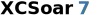
\includegraphics[angle=0,width=0.66\textwidth,keepaspectratio='true']{graphics/title.pdf}
    \end{center}
    \begin{center}
      \normalfont\huge\textsf{O computador de vôo de código aberto}\par
    \end{center}
    \vskip 1cm
    \begin{center}
      \normalfont\huge\textsf{\@title}\par
    \end{center}
    \vskip 1cm
  \end{maxipage}

  \vfill
  \todo[nolist,size=\Large,inline]{Draft state, better you wait printing the
  whole manual}

  \begin{flushright}
    \large \strut {
      \sf
      \today \\
      For XCSoar version \version \\
      \xcsoarwebsite{} \\
    } 
    \par
  \end{flushright}
  \par
  \vfil
  \vfil
  \null
  \cleardoublepage
}

\usepackage[utf8]{luainputenc}
\usepackage{makeidx}\makeindex

\begin{document}

%%%%%%%%%%%%%%%%%%%%%%
% Front page
\maketitle

%%%%%%%%%%%%%%%%%%%%%%
% Table of contents
\begingroup
\fontfamily{ptm}
\normalsize
\fontseries{c}\selectfont
\setlength{\parskip}{0.05\baselineskip}
\tableofcontents
\endgroup


%%%%%%%%%%%%%%%%%%%%%%
\chapter*{Preface}

\section*{Warnings and precautions}

\warning IT IS THE USER'S RESPONSIBILITY TO USE THIS SOFT\-WARE PRUDENTLY. THIS SOFTWARE IS 
INTENDED TO BE USED ONLY AS A NAVIGATION AID AND MUST NOT BE USED FOR ANY PURPOSE REQUIRING 
PRECISE MEASURE\-MENT OF DIRECTION, DISTANCE, LOCATION, OR TOPO\-GRAPHY. THIS SOFTWARE SHOULD 
NOT BE USED AS AN AID TO DETERMINE GROUND PROXIMITY FOR AIRCRAFT NAVIGATION. THIS SOFTWARE 
SHOULD NOT BE USED AS A TRAFFIC COLLISION AVOIDANCE SYSTEM.



%%%%%%%%%%%%%%%%%%%%%%
\section*{Legal notices}

\subsection*{Software license agreement}

This software is released according to the GNU General Public License
Version~2.  See Appendix~\ref{cha:gnu-general-public} for the full
text of the agreement and warranty notice.

\subsection*{Limited liability}

In no event shall XCSoar, or its principals, shareholders, officers,
employees, affiliates, contractors, subsidiaries, or parent
organizations, be liable for any incidental, consequential, or
punitive damages whatsoever relating to the use of the Product.

\subsection*{Disclaimer}
This product, and all accompanying files, data and materials, are
distributed "as is" and with no warranties of any kind, whether
express or implied.  This product is used entirely at the risk of the
user.  Although great care has been taken to eliminate defects during
its development it is not claimed to be fault-free. No claims are made
regarding its correctness, reliability or fitness for any particular
purpose.  The XCSoar project developers and contributors shall not be
liable for errors contained herein or for incidental or consequential
damages, loss of data or personal injury in connection with
furnishing, performance, or use of this material.


%%%%%%%%%%%%%%%%%%%%%%
\chapter{Introdução}\label{cha:introduction}
Este documento é um manual do XCSoar para o piloto, um computador de vôo de código aberto que foi originalmente desenvolvido para dispositivos “Pocket PC”.  É assumido que o público-alvo deste manual deve ter um conhecimento das teorias fundamentais de vôo livre, e um conhecimento básico sobre o vôo de distância (Cross Country).

As atualizações do software XCSoar podem resultar em desatualizações em alguma parte deste manual.   Você deve ler a notas emitidas distribuídas com o software para saber das alterações.  As alterações e atualizações estão disponíveis em:  
\begin{quote}
\xcsoarwebsite{}
\end{quote}

\section{Organização deste manual}

\todonum[inline]{Write about the manual crossref hinting icons and the yellow
colour. The Quickstart will be readable also without those links available} 
Este manual notadamente foi escrito com o propósito de possibilitar ao usuário do XCSoar iniciar rapidamente bem como apoiar seu profundo conhecimento de todas as características, conceitos e táticas introduzidas.  A todo tempo, os autores têm feito esforços para desenvolver este software sob a perspectiva do piloto (e honestamente espero que tenha tido sucesso).

Os autores encorajam você a dispender um tempo lendo todo o manual, capítulo por capítulo (com exceção dos capítulos de referência e Configurações).  Sinta-se seguro, o tempo que irá dispender irá recompensar o aumento do conhecimento.  Na leitura, poderá se sentir um pouco entediado.  Por este motivo os autores introduziram alguns itens “anti-tédio”: links e ícones.

\begin{figure}[h]
\centering
\includegraphics[width=0.8cm,angle=0,keepaspectratio='true']{figures/config.pdf}
\hspace{1.5cm}
\includegraphics[width=0.8cm,angle=0,keepaspectratio='true']{figures/reminder.pdf}
\hspace{1.5cm}
\includegraphics[width=0.8cm,angle=0,keepaspectratio='true']{figures/gesture.pdf}
\hspace{1.5cm}
\includegraphics[width=0.8cm,angle=0,keepaspectratio='true']{figures/warning.pdf}
\caption{Icons configuration, reminder, gesture, warning}
\end{figure}

\warning Atenção.  O ícone atenção é usado sempre que se necessita seguir as instruções precisamente.   Não seguir as instruções significa resultados inesperados, disfunções totais ou mesmo perigo à vida.  Só prossiga se o item foi entendido.

\gesture{DU} Gesto.  O gesto de deslize está disponível utilizando uma tela sensível ao toque para ativar um menu ou função, entre outros.  Neste exemplo, o padrão DU significa mover a ponta do dedo para baixo e para cima (em linhas retas) na tela.
  
\gesturespec{du} Gesto específico.  Toda vez que o autor do manual se refere ao desenvolvimento rápido na escrita, o ícone é fornecido representando os movimentos.

\tip Lembrete. Este ícone identifica uma dica, truque ou coisas que você deve se lembrar após ter lido as seções correspondentes.

\config{orientation} Veja a configuração…. O ícone representa duas ferramentas e a descrição dos itens mencionados e como configurá-los.  Os números ao lado do ícone referem-se ao capítulo/seção específicos do manual, neste caso ao Capítulo\ref{cha:infobox} e \ref{cha:configuration}, neste caso se referindo à seção \ref{conf:orientation}. 

\marginlabel{\parbox{1.3cm}{\rotatebox[origin=c]{180}{\includegraphics[width=0.9cm]{figures/warning.pdf}}}}
\rotatebox[origin=c]{180}{Pare de ler manuais enquanto voa!}

\emph{Leia} em casa, \emph{configure} configure no chão, em segurança.  Se percebeu esta advertência de ponta cabeça, você está pronto para prosseguir.

\config{usingxcsoarsafely} Referindo-se ao segundo caso de exemplo do ícone “Configuração” à esquerda, o ícone refere-se ao capítulo \ref{cha:introduction}, (this Capítulo), seção 
\ref{sec:usingxcsoarsafely}, "Usando o XCSoar com segurança" que pode ser entendido “como configurar por si mesmo”.  Está sob sua responsabilidade em se aprofundar mais em conhecimentos ou simplesmente prosseguir.  Se estiver lendo este documento eletronicamente, clique no número do capítulo/seção e automaticamente será direcionado ao mesmo.  

Os números são impressos em azul, bem como os ícones introduzidos, significando “ajuda disponível”, bem como outros localizadores de recursos, sublinhados com texto azul. Clicando no texto como  \xcsoarwebsite{/contact} abrirá a página da internet ou e-mail para entrar em contato com outras fontes ou pessoas relativas ao desenvolvimento deste.

O lembrete desta “Introdução” é para deixar você preparado para o XCSoar, aumentar seu nível de conhecimento e manter suas habilidades.   
Capítulo \ref{cha:quickstart} "Início Rápido" deve ser o próximo ponto depois do capítulo 
\ref{cha:installation} "Instalação" para usuários com urgência. Sinta-se à vontade para criar atalhos, mas não resuma tanto a leitura que não veja:

Capítulo~\ref{cha:interface} que introduz o conceito de interface de usuário e fornece uma visão geral da tela. .

Capítulo~\ref{cha:navigation} que descreve o mapa dinâmico na tela em grandes detalhes e também como o software pode ajudar na navegação geral.  Capítulo~\ref{cha:tasks} descreve como as provas de cross-country são detalhadas e voadas, e apresenta algumas ferramentas de análise para aumentar o seu desempenho.
Capítulo~\ref{cha:glide} apresenta detalhes das funções do computador de planeio e é importante para os pilotos se atentarem de como o computador realiza seus cálculos.

Capítulo~\ref{cha:atmosph} descreve como o computador pode fazer a interface com o variômetro e outro sensor de dados aéreo e como utiliza estas medições para desenvolver modelos de atmosferas de vento e convecções térmicas.  
Capítulo~\ref{cha:airspace} descreve como o XCSoar pode ajudar a gerenciar o vôo, especialmente usando espaço aéreo e o sistema de colisão FLARM.  Capítulo~\ref{cha:avionics-airframe} descreve sobre sistema de integrações e diagnósticos do sistema, a integração do XCSoar com dispositivos de comunicação e com sensores de vento.

O lembrete deste manual contém principalmente material de referência.  
Capítulo~\ref{cha:infobox} relaciona todos os tipos de informações que podem ser apresentadas no campo de dados próximo ao mapa.  A configuração do software é descrita em detalhes no
Capítulo~\ref{cha:configuration}.  Os formatos de vários arquivos de dados que o programa usa, bem como obtê-los e editá-los, está descrito no Capítulo~\ref{cha:data-files}.

Finalmente, uma breve história e discussão sobre o processo de desenvolvimento do XCSoar está no Capítulo~\ref{cha:history-development}.

\section{Notas}

\subsection*{Terminologia}
Uma variedade de termos pode ser utilizada para descrever dispositivos embutidos como a plataforma Pocket PC, incluindo “organizadores/agendas”,   PDAs (Assistente Portátil Digital) e PNA (Assistente Pessoal de Navegação).  O XCSoar também está disponível no computador de vôo Altair, da Triadis Engineer, que é formado por um sistema eletrônico de instrumentos de vôo e outras várias plataformas.  
Completando este documento estes termos são usados alternadamente para se referirem qual o hardware em que o XCSoar está rodando.


\subsection*{Capturas de tela}
Para completar este manual, há diversas capturas de tela do XCSoar.  Foram retiradas do programa em funcionamento em várias plataformas e possivelmente em diversas versões.  Cada plataforma e versão poderá ter resoluções de tela diferentes, layouts e fontes, e poderão apresentar pequenas diferenças na aparência da tela.  A maioria das capturas de tela foram retiradas do XCSoar rodando em modo paisagem.

\section{Plataformas}
\begin{description}
\item[Windows Mobile PDA/PNA]
Dispositivos com Microsoft Pocket PC 2003 até o Windows Mobile 6 rodam o XCSoar.   Windows Mobile 7 não suporta o XCSoar, pois a Microsoft decidiu não estender o suporte para aplicativos de versões anteriores.
\item[Dispositivos Android]
XCSoar roda em Android 1.6 ou superior.
\item [Leitores eBook]
XCSoar roda em alguns dispositivos Kobo eReader.  Uma porta nativa foi lançada com a versão 6.7.1, mas é ainda considerada experimental.
\item[Altair]
O computador de vôo Altair da Triadis Engineering é um computador que vem de fábrica com o XCSoar instalado.  A versão Altair PRO também contém um GPS interno.
\item[Windows PC]
É possível rodar o XCSoar em um computador normal com o Sistema operacional Windows.  O ajuste pode ser usado para treinar a si mesmo a usar o XCSoar.  O modo de simulação está incluso no XCSoar bem como a função de replay do vôo (IGC), que pode ser usada quando não está conectado à uma fonte de GPS válida.
\item[Unix/Linux PC]
o XCSoar pode ser rodado com o sistema Unix, com o simulador Wine.  Uma porta nativa de Unix foi lançada com a versão 6.0 do XCSoar, mas é considerada experimental.
\end{description}



\section{Suporte Técnico}

\subsection*{Resolução de problemas}
Um pequeno time de dedicados desenvolvedores produzem o XCSoar.  Todavia, estamos felizes em ajudar com o uso do nosso software, nós não podemos lhe ensinar sobre o básico da tecnologia da informação.  Se você tem alguma pergunta particular sobre o XCSoar não descrita neste manual, por gentileza entre em contato.  Você irá achar todos os links resumidos em:
\begin{quote}
\xcsoarwebsite{/contact}
\end{quote}
Para iniciar a comunicação, inscreva-se no fórum do XCSoar em:
\begin{quote}
\url{http://forum.xcsoar.org}
\end{quote}
Se a sua questão aparentemente não foi listada, mande-nos um e-mail:
\begin{quote}
\href{mailto:xcsoar-user@lists.sourceforge.net}{xcsoar-user@lists.sourceforge.net}
\end{quote}
Algumas perguntas frequentes serão adicionadas a este documento e à seção FAQ (Questões frequentes perguntadas) no site do XCSoar.  Você poderá também achar útil se inscrever na lista de discussões do XCSoar, para se atualizar dos últimos desenvolvimentos.

Se tudo isso não ajudar, provavelmente você descobriu uma falha.



\subsection*{Retorno}
Como todo software complexo, o XCSoar pode estar sujeito à falha, então se você achar algum, por favor reporte aos desenvolvedores do XCSoar utilizando nosso portal para falhas em:
\begin{quote}
\xcsoarwebsite{/trac}
\end{quote}
ou nos enviando um e-mail para: 
\begin{quote}
\href{mailto:xcsoar-devel@lists.sourceforge.net}{xcsoar-devel@lists.sourceforge.net}
\end{quote}
O XCSoar arquiva muitos dados valiosos em um arquivo de log 
\verb|xcsoar.log| no diretório \texttt{XCSoarData}. O arquivo de log pode ser anexado ao e-mail para ajudar os desenvolvedores do XCSoar a determinar a causa do possível problema.  Para usuários do Altair, o arquivo de log é transferido do diretório “FromAltair” pelo AltairSync, se um drive USB for plugado quando o Altair é ligado pela primeira vez.  Se você gostou da idéia de fazer mais, envolva-se em:
\begin{quote}
\xcsoarwebsite{/develop}
\end{quote}

\subsection*{Atualizações}
Você deve periodicamente visitar o site do XCSoar para verificar se há atualizações para o programa.  O procedimento de instalação descrito acima pode ser repetido para que haja a atualização do software.  Todas as configurações, ajustes, dados e arquivos serão preservados durante a instalação/atualização.

Também é recomendado que periodicamente verifique por atualizações nos arquivos de dados, particularmente o Espaço Aéreo, que pode estar sujeito às mudanças pelo departamento de aviação civil.

\subsection*{Atualização do XCSoar no Altair}
Atualizar o XCSoar no Altair envolve baixar o último arquivo de programa {\tt XCSoarAltair-YYY-CRCXX.exe}, copiando para uma memória USB, quando se usa o utilitário AltairSinc no dispositivo Altair para completar a instalação.  Veja no manual do usuário do Altair para detalhes.
Outros dados e arquivos de programas podem ser transferidos de modo similar a este.

Outros dados e arquivos de programas podem ser transferidos de modo similar a este.

\section{Treinamento}
Para sua própria segurança e de outros, os pilotos que utilizam o XCSoar são alertados para fazerem treinamento de como utilizar o XCSoar no solo e se familiarizarem com sua interface e características antes de voarem.

\subsection*{Usando o XCSoar no PC}
A versão do XCSoar para PC deve ser usada para se tornar familiar com a interface do XCSoar e suas funcionalidades no conforto de suas residências.  Todos os arquivos e configurações usados por esta versão são idênticas às versões incorporadas, portanto pode ser útil experimentar algumas customizações na versão PC antes de usá-las em vôo.

A versão para PC também pode ser conectada aos dispositivos externos e operar exatamente igual às versões internas.  Algumas sugestões de uso incluem:
\begin{itemize}
\item Conecte o PC a um dispositivo FLARM e use o XCSoar como uma estação em solo para mostrar o tráfego de aeronaves que usam FLARM.
\item Conecte o PC a um variômetro inteligente como o Vega para testar as configurações e ajustes do variômetro.
\end{itemize}

\subsection*{Usando o XCSoar como um simulador de vôo}
Uma boa maneira de aprender como usar o XCSoar é conectar o dispositivo Pocket PC a um computador que esteja rodando um simulador de vôo que possa fornecer dados NMEA a uma porta serial.  Alguns simuladores que funcionam dessa forma são Condor e X-Plane. 

O benefício desta forma de treinamento é que o XCSoar pode ser utilizado em modo FLY, comportando-se como se você estivesse realmente voando e você pode sentir como o programa funciona enquanto voa no simulador.

\section{Usando o XCSoar com segurança}\label{sec:usingxcsoarsafely}\label{conf:usingxcsoarsafely}
O uso de um sistema interativo como o XCSoar em vôo carrega consigo certos riscos devido ao potencial de distração que pode ocorrer com o piloto quando mantém sua atenção e olhos no cockpit.

A filosofia que guia o projeto e desenvolvimento do software é de tentar reduzir esta distração, minimizando a necessidade de interação do usuário ao mínimo, e apresentando informações de uma maneira clara e de fácil interpretação.

Pilotos usando XCSoar devem ser responsáveis por usar o sistema com segurança.  Boa prática no uso do XCSoar inclui:

\begin{itemize}
\item Tornar-se familiarizado completamente com o sistema através de treino no solo.
\item Desempenhar curvas claras antes de interagir com o XCSoar em vôo, para que tenha certeza que não há risco de colisão com outro quando em tráfego aéreo.
\item Ajustar todo o sistema para tirar vantagem das funções automáticas e entrada de eventos, para que a interação do usuário seja minimizada.  Se você está fazendo algumas interações constantes no sistema, pergunte a outros usuários do XCSoar se o software faz estas interações automaticamente.
 

\end{itemize}


%%%%%%%%%%%%%%%%%%%%%%
\chapter{Installation}\label{cha:installation}

\section{To run XCSoar}
 you need to obtain the following:

\begin{itemize}
\itemsep0em
\item a device to run XCSoar on
\item XCSoar
\item a GPS receiver
\item a waypoint file
\item an airspace file (optional)
\item a map file (optional)
\end{itemize}

\section{! Before you go out flying the first time with XCSoar !}

After having installed XCSoar successfully, you might use it instantly. XCSoar 
will launch with a ready-to-use pre-configuration. But be aware, that up to 
this point your new toy will give you a moving map display only.
\warning \emph{Don't trust the computations.} You have to tell XCSoar which 
plane you are flying in advance.  This is done by specifying your plane's data 
as are polar, weight and some other data.  However it's always a good idea to 
study the manual and become familiar with XCSoar at home.

\section{How to get the most from XCSoar}

In order to achieve your maximum benefit from XCSoar, you are kindly asked to 
do do some more after having installed the software and downloaded some data 
files. ``Some more'' includes personal and plane data as well as configuration 
of just a few features. Unless you are willing to tweak everything XCSoar 
provides, this could be done in a rather short time. Necessary steps are 
summarized in an \emph{XCSoar Checklist}, given in the next chapter.

If you are planning to arrange a system with several components engaged in, 
this manual will give you valuable advice on both, how to set up things and how 
to use them.

If you are a pilot in a hurry, the authors suggest to change to the short form 
manual \texttt{XCSoar-in-a-Flash} going through the \emph{XCSoar Checklist} 
step by step. The short form manual is available on \url{http://www.xcsoar.org/
discover/manual.html}.



\section{XCSoar Checklist}

\subsection*{{Bring XCSoar into play}}
\begin{itemize}
\item get hardware and install XCSoar
\item get appropriate data files of your flight district
\item tell XCSoar which data files to use
\item tell XCSoar about the glider's polar \& weight
\item possibly connect to instruments
\item finish setup and familiarize
\item mount hardware
\item add items listed underneath to your checklists
\item make "home"
\end{itemize}

\subsection*{Conduct preflight check, including}
\begin{itemize}
\item setup polar and weight
\item setup wind and flight parameters (MC, bugs, QNH)
\item possibly setup a task
\end{itemize}

\subsection*{Conduct start check, including}
\begin{itemize}
\item Check wind and flight setup once more
\end{itemize}
\vspace{2em}

\subsection*{Fly, enjoy}
\vspace{4em}

\subsection*{Conduct after flight check}
\begin{itemize}
\item Download flight logs from logger, upload to skylines and OLC
\item Gather statistical data of flight.
\end{itemize}
\newpage




\section{Compatibility}

\subsection*{Devices for running XCSoar}

XCSoar runs on the following platforms:

\begin{itemize}
\item PDAs with Pocket PC 2000, 2002, 2003 \\
  Example: iPaq 3800, iPaq 3900
\item PDAs with Windows Mobile \\
  Example: iPaq hx4700, Dell Axim x51v
\item PNAs with Windows CE 3.0 or newer \\
  Example: HP314, Mio400
  \item Android mobile phones and tablets with Android 1.6 or newer \\
  Example: Dell Streak, Samsung Galaxy S II, HTC Desire HD,
  Motorola Xoom
\item eReader Kobo (experimental, Dec. 2013)
\item Triadis Altair
\item LX MiniMap
\item Windows 2000 or newer
\item Linux
\item Mac OS X (outdated)
\end{itemize}

\subsection*{GPS, Logger, Vario}

XCSoar is compatible with any GPS emitting NMEA data.  Most modern
Android devices have a built-in GPS, but for several reasons it is favorable to
connect to one or more external devices:

\begin{itemize}
\item a specialized GPS receiver gains much better reception providing much 
better data for measures and calculations
\item an airspeed indicator allows quick and exact wind estimates
  without circling
\item a vario improves the thermal assistant
\item a task can be declared to an IGC logger, and after landing, the
  flight log can be downloaded
\item some varios allow synchronising the MacCready setting with
  XCSoar
\item flarm (and even ADS-B input) provide informations and stati of others 
around you (- and of course Flarm gives you collision detection)
\end{itemize}

\subsection*{Supported external devices and features}
\label{sec:supported-varios}

\newcommand{\y}[0]{{ $\surd$ }}
%{0.8\textwidth}
\noindent\makebox[\textwidth]{%
\begin{tabular}{l|ccc|cc|cc|c}
       \multicolumn{1}{r}{Supported:} & \multicolumn{3}{c|}{-Features} & \multicolumn{5}{c}{-Stream Data} \\
NMEA Device & 
  \begin{sideways} Declaration\end{sideways} & 
  \begin{sideways} Remote ctrl.\end{sideways} & 
  \begin{sideways} Download\end{sideways} &
  \begin{sideways} Airspeed\end{sideways} & 
  \begin{sideways} Vario\end{sideways} & 
  \begin{sideways} Baro. altitude\end{sideways} & 
  \begin{sideways} Wind\end{sideways} &
  \begin{sideways} G-Sensor\end{sideways} \\
\hline
%                    _Decl_Remo_Down_Airs_Vari_Baro_Wind_Gsen_
Borgelt B50          &    & \y &    & \y & \y & \y &    &    \\
CAI 302              & \y & \y & \y & \y & \y & \y & \y & \y \\
CAI GPS Nav          &    &    &    &    &    &    &    &    \\
Condor               &    &    &    & \y & \y & \y & \y &    \\
\hline
Digifly Leonardo     &    &    &    & \y & \y & \y & \y &    \\
EW Logger            & \y &    &    &    &    & \y &    &    \\
EW microRecorder     & \y &    &    &    &    & \y &    &    \\
FLARM                & \y &   & \y  &    &    & \y &    &    \\
\hline
%                    _Decl_Remo_Down_Airs_Vari_Baro_Wind_Gsen_
Flymaster F1         &    &    &    &    & \y & \y &    &    \\
Flytec 5030          &    &    &    & \y & \y &    &    &    \\
GTAltimeter          &    &    &    &    &(\y)& \y &    &    \\
ILEC SN10            &    &    &    &    & \y & \y & \y &    \\
\hline
IMI ERIXX            & \y &    & \y &    &    &    &    &    \\
LX20, Colibri        & \y &    & \y &    &    & \y &    &    \\
LXNAV Nano           & \y &    & \y &    &    &    &    &    \\
\hline
%                    _Decl_Remo_Down_Airs_Vari_Baro_Wind_Gsen_
LXNAV V7             &    & \y &    & \y & \y &    &    &    \\
PosiGraph            & \y &    &    &    &    & \y &    &    \\
Triadis Altair (pro) & \y &    &    &    &    & \y &    &    \\
Triadis Vega         &    & \y &    & \y & \y & \y &    & \y \\
\hline
Vaulter              &    & \y &    & \y & \y & \y & \y & \y \\
Volkslogger          & \y &    & \y &    &    & \y &    &    \\
Westerboer VW1150    &    & \y &    & \y & \y & \y &    &    \\
Westerboer VW921, 922
                     &    & \y &    & \y & \y & \y &    &    \\
\hline
Zander / SDI         &    & \y &    & \y & \y & \y & \y &    \\

\end{tabular}}
\footnotetext{LX Navigation offers a variety of intelligent vario 
  devices such as LX1600, LX5000, LX7000. They all share their NMEA functionality. 
  The offered functionality in connection to XCSoar depends on 
  last not least e.g. the vario's firmware revision. }

While most Windows CE based devices have a serial port, such legacy
hardware is not present in modern Android devices.  Those can either
use Bluetooth or the Android IOIO board.  To use Bluetooth, you need
to connect the external device to a Bluetooth-to-Serial adapter, such
as the K6-Bt or the Glidertools VFBT-1.


\section{Software installation}

The software is available as a free download from the XCSoar website
~\xcsoarwebsite{}.  This section describes which file should be
downloaded, and how to install it.

\subsection*{On Android}

Obtain XCSoar from Google's Android market, or install the \verb|apk|
file manually.  Copy the data files on the SD card in the directory
\verb|XCSoarData|.

\subsection*{On a Kobo Mini}

The Kobo Mini is a cheap e-book reader.  It has a black and white
e-paper screen with excellent sunlight readability.

Before you begin: back up the internal SD card.  The XCSoar installer
may break the Kobo, though unlikely.  You can always recover the Kobo
from a software failure, but only if you have access to a backup.

To install XCSoar, connect the Kobo to your PC via USB.  The Kobo
exposes a mass storage device to your PC; open it and create a
directory called \texttt{.kobo} (note the leading dot).  Download the
file \texttt{KoboRoot.tgz} from the XCSoar website into that
directory (\url{http://www.xcsoar.org/hardware/}). Unplug the Kobo and reboot it (switch it off completely,
and switch it on again).  You will see the message ``Updating'', and
after a few minutes, the Kobo shows a menu that allows you to launch
XCSoar or the Kobo e-book reader software.

To copy data files (maps, waypoints, ...) to the Kobo, launch the
original Kobo software (``Nickel'') and connect the Kobo to your PC
again.  Copy the files into a directory called \texttt{XCSoarData} at
the top level.

Alternatively data files may be downloaded via XCSoar's file manager, after having invoked a W-LAN-connection just before launching XCSoar.  

\subsubsection{Hacking the Kobo}

After installing XCSoar on the Kobo, the new boot script checks for a
script called \texttt{XCSoarData/kobo/init.sh} and executes it.  If
you know what you're doing, you can use this script to do things at
boot time, for example launch \texttt{inetd} (for \texttt{telnet}
access).

When you launch \texttt{Nickel} (the original e-book firmware), the new
boot script also checks for a script called
\texttt{XCSoarData/kobo/init_nickel.sh} and executes it. Again, if
you know what you're doing, you can use this script to do things
before \texttt{Nickel} is fully started, for example send commands
to your attached vario (to shut it down, to cut the volume, etc...).

\subsection*{On a PDA (Windows Mobile, PocketPC)}

Choose one of the targets:

\begin{description}
\item[\texttt{PPC2000}] Pocket PC 2000/2002, Windows CE 3.0
\item[\texttt{PPC2003}] Pocket PC 2003, Windows CE 4.0
\item[\texttt{WM5}] Windows Mobile 5 or newer
\item[\texttt{WM5X}] Windows Mobile 5 or newer with XScale CPU or
  better (e.g. hx4700)
\end{description}

Download the program file \verb|XCSoar.exe| to a SD card.  You can
launch it with the File Explorer.
\sketch{figures/XCS_Today.png}
Another method to install XCSoar on a PDA is the CAB file.  Download
it to the SD card.  Use the File Explorer to install it.  After the
installation, the XCSoar `FLY' and `SIM' launcher icons will be
visible on the Today screen.


\subsection*{On a PNA (Windows CE)}

Download the program file \verb|XCSoar.exe| (target ``WM5'') to a SD
card.  You can launch it with the File Explorer.

\subsection*{On a Windows PC}

Download the program file \verb|XCSoar.exe| (target ``PC'') to your
hard disk.

\subsection*{On Unix/Linux}

The file downloaded is \verb|xcsoar_XXX.deb|, where \verb|XXX| includes
the version number and platform, e.g. \verb|xcsoar_6.0.4_i386.deb|.
The is a Debian package and can be installed using 
\begin{center}
\verb|sudo dpkg -i xcsoar_XXX.deb|.
\end{center}
Use \verb|dpkg-query -L xcsoar| to see where the executable and 
other files are installed,
Additional data files must be placed in the directory
\verb|~/.xcsoar|.
If \verb|~/.xcsoar| does not exist, it will be created the first time
that \verb|xcsoar| is run.

\subsection*{On Raspberry Pi and Cubieboard}

Install the Debian package as described above.  However, unlike on
``regular'' Linux, XCSoar will not use X11.  Instead, it runs
full-screen on the Linux console.

XCSoar requires access to your input devices
(\texttt{/dev/input/event*}).  By default, only \texttt{root} is
granted access.  To override this, create a \texttt{udev}
configuration file, e.g. \texttt{/etc/udev/rules.d/99-input.rules}:

\begin{verbatim*}
KERNEL=="event*", NAME="input/%k", MODE="660", GROUP="input"
\end{verbatim*}

Create the group \texttt{input} and make your user a member:

\begin{verbatim*}
groupadd input
adduser pi input
\end{verbatim*}

\section{Data files}\label{sec:data files}

To be able to use XCSoar's advanced features, additional data files, such as
terrain, topography, special use airspace, waypoints etc.\ are needed. The files
that can be used with XCSoar are described in Chapter~\ref{cha:data-files}.

All data files should be copied into the directory
\texttt{XCSoarData}.  This directory must be in a specific place
so that XCSoar knows where to look for data files:

\begin{description}
\item[Windows PC]
\texttt{XCSoarData} is in your personal folder (``\texttt{My
Documents}'')
\item[Windows Mobile PDA/PNA]
If there is a directory named \texttt{XCSoarData} in the same
directory as \texttt{XCSoar.exe}, then this one will be used.
\texttt{XCSoarData} is on the SD card.  If there is no SD card, then
XCSoar looks for it in \texttt{My Documents}.
\item[Unix/Linux]
The directory is called \verb|.xcsoar| in the user's home directory.
\item[Android Devices]
\texttt{XCSoarData} is on the SD card.
\item[Altair]
If XCSoarData exists on an USB drive, that one is used, otherwise the
internal storage is used.
\end{description}


XCSoar will generate a number of additional files at run time.  These
will be placed in the  \texttt{XCSoarData} directory (Windows PC, 
Windows and Android mobile devices), or the \texttt{.xcsoar} directory (Unix/Linux
PC).  From the first run, XCSoar will create and maintain the files 
\texttt{Default.tsk} (Default Task),  
\texttt{default.prf} 
(configuration settings),
\texttt{xcsoar.log}, 
plus three directories: \texttt{cache},
\texttt{config} and \texttt{logs}.  Additional files may be
created/modified while XCSoar is running, such as task files
(\texttt{*.tsk}) and flight logs.


\section{Running XCSoar}
%\subsection*{Fly and simulator modes}

Two modes are available inside the XCSoar application: 
\begin{description}
\item[FLY] This mode is used when actually flying.  The simulator is 
  disabled and serial communications are active. 
\item[SIM] This starts XCSoar in simulator mode, no serial communications
  are attempted.
\end{description}

\subsection*{Altair version}
XCSoar starts up automatically when Altair is powered on.
The PWR/ESC button (top left) has multiple functions:
\begin{description}
\item[Powering on]  Press and hold the PWR/ESC button for one second.
  The LED in the button will light up, and XCSoar will start after
  Altair has booted.
\item[Powering off]  Press and hold the PWR/ESC button for 3 seconds.
  Altair will switch off.
\item[Escape] Pressing the PWR/ESC button quickly acts as an
Escape key, typically used to close dialog pages or as a cancel function.
\end{description}

The Altair version of XCSoar does not include a simulator mode.

\subsection*{XCSoar PC version}
The program can be run by opening the explorer window, finding the directory
that has the XCSoar.exe executable, and double clicking on that program file.

The program command line options allows the screen orientation of
the display to be defined:
\begin{description}
\item[-portrait] The screen is 480 pixels wide, 640 pixels high.
\item[-square] The screen is 480 pixels wide, 480 pixels high.
\item[-landscape] The screen is 640 pixels wide, 480 pixels high. This is the
usual setting. If you don't specify this parameter the landscape version will be
loaded automatically.
\item[-small] Draws the screen at half size.  This is useful for using XCSoar in
 conjunction with flight simulators e.g.\ Condor.
\end{description}
To change the screen orientation, it is convenient to create a shortcut to the
program, then right click on the shortcut icon and click on ``Shortcut''. 
In the field ``Target'' add one of the desired options listed above.

\subsection*{XCSoar Unix/Linux PC version}
Run \verb|xcsoar| from a command line, or create a shortcut on the
desktop.  The location of the executable file may be found using
\verb|which xcsoar|.  Only landscape mode is  supported for now.

\subsection*{Loading data files}\label{sec:loaddatafiles}
The first time that XCSoar is run, it does not automatically load the 
data files that you placed in the \verb|XCSoarData| directory.  
To tell XCSoar which files to load, double click/tap the map (the large,
blank white part with the glider symbol in the center),
choose the menu \bmenug{Config 2} (click/tap it twice), then select the item 
\bmenug{System}.  The Configuration screen should be displayed:
\sketch{figures/config-basic.png}
The first page allows you to choose the map, 
waypoint and airspace files, by clicking/tapping on the text boxes.
Many other features of XCSoar may be configured here. These are described in detail in Chapter
\ref{cha:configuration}.
Once completed, XCSoar reloads those files; from now on, the data files
will be loaded automatically at run time.

\subsection*{Start-up and user profiles}\label{sec:profiles}
When XCSoar starts up, it will check for existing profiles. If multiple
profiles are detected it will displays a small window asking you which profile
to load. To proceed, choose the desired profile and press Enter. If no
profile is chosen the settings from the last session are loaded again. Profiles
can be useful for example in the following cases:
\begin{itemize}
\item Different pilots
\item Competition versus casual flying
\item Flying in different locations
\item Different planes (with different polars)
\end{itemize}
Profiles also might be understood as preserving a backup of a certain 
configuration. Virtually every of XCSoar's settings is stored in a profile 
file with extension \texttt{.prf}. Once you are happy with all your settings, 
make two copies of your profile file. One carrying extension \texttt{.prf}, 
the second copy carrying extension \texttt{.bak}.
Whereas the \texttt{.prf} file will show up on startup and reflect all of 
your changes made whilst XCSoar is running for the next startup, the file 
\texttt{.bak} will keep the settings, you judged being worth it to preserve. 
As an example you might create a set of files as is:
\begin{itemize}
\item \texttt{buddiesinArcus.prf}
\item \texttt{buddiesinArcus.bak}
\item \texttt{johninKa6atwonderland.prf}
\item \texttt{johninKa6atwonderland.bak}
\end{itemize}

\subsection*{SIM mode}
XCSoar comes with a simple interface allowing for conducting a simulated 
flight. Depending on the hardware platform, there are different 
methods for altering values of bearing, speed, an height.  Simulation is 
intended for your first familiarization with XCSoar in action. If you like the 
idea simulating a more realistic thing at home, you should acquire a "true" 
soaring simulator, to be connected to XCSoar.

On the map screen, clicking/touching the glider symbol
with touchscreen or mouse and dragging 
causes the glider to move in the direction of the drag, the
speed being proportional to the length of the drag.

With buttons, the aircraft
speed, altitude and direction may be changed using the Infoboxes.
The following may not be available in total on every hardware platform, but on 
any of the platforms XCSoar supports, a full set of inputs needed for 
simulation purposes is possible.

By pushing an Infobox, you select a value to be altered by buttons, either 
 hardware or menu buttons.
The aircraft altitude can be adjusted by selecting the GPS altitude
InfoBox \bmenuw{Alt GPS}, and touching the up or down key or buttons on the 
touchscreen.
The airspeed can be adjusted by selecting the Infobox ground speed
\bmenuw{V Gnd}, touching up or down key or menu buttons.
The glider's track  can be adjusted by selecting the track InfoBox
\bmenuw{Track}, and touching up/down buttons.

With either of the \bmenuw{Alt GPS} or \bmenuw{V Gnd}
selected, the glider's direction may be changed using the left/right keys.

Other controls, buttons and menus work the same as in FLY mode.


\subsection*{Splash screen}
When XCSoar starts up, shuts down, or loads large files, such as airspace,
waypoints, terrain, etc., a progress screen is presented while the data is being
loaded. This screen has a progress bar which indicates the data loading
activity, and a short line of text describing the action that is being performed.

This screen also displays the software version information.

\subsection*{Exiting the program}
For PDA and PC versions, XCSoar is shut down from the menu. The menu can be
opened by double-clicking on the map or the \InfoBox es.
\begin{quote}
\bmenug{QUIT}
\end{quote}

For PC versions, XCSoar can also be shut down by clicking the close icon
on the XCSoar window.

For Altair, XCSoar is shut down by holding the PWR button for two seconds or
more.


%%%%%%%%%%%%%%%%%%%%%%
\chapter{User Interface}\label{cha:interface}
\begin{figure}[h]
\includegraphics[angle=0,width=\linewidth,keepaspectratio='true']{figures/plain.png}
\caption{Typical XCSoar main screen layout}
\end{figure}

This chapter describes the fundamental user interface concepts used by 
XCSoar, and is intended as an overview. The \emph{main screen} covers much of 
the information needed during normal flight.  Typically, the main screen is 
composed of the moving map and infoboxes. For several reasons - not being the 
scope of an introduction - you have a choice of using several main screens 
in-flight, named \emph{screen pages}.

Screen pages are easily accessed by a horizontal swipe gesture just like 
turning pages of a book or button push, depending on the hardware you use. 
With screen pages you are enabled to compose several main screens to be used 
advantageously in different situations in-flight. Simply speaking, you are 
enabled to use appropriate information in different \emph{use cases}, to be 
accessed quite simply and fast. 

Whenever actual situations are worthy of grabbing the pilot's attention, an 
\emph{overlay} is put in front of the main screen. This happens especially 
when urgent reaction by the pilot is required as are the situation of a 
possible collision or an entering of a restricted airspace expected to happen
soon.

Evidently, menu buttons and menu screens are overlays too, and there are many 
more. As a result, the elements put on each other form a display stack with 
the main screen representing the base of it. More detailed descriptions are 
given in following chapters.



\section{Display elements}
\subsection*{Main screen and screen pages}
Every screen page out of XCSoar's screen pages' ensemble is composed of several 
parts:
\begin{description}
\item[Main area] The bulk of the screen typically is dedicated to the GPS moving 
map display. Various symbols relating to glide computer information are overlaid 
the map area. Icons and text may appear along the lower edge of the screen
to indicate status of connected devices, flight modes etc.
Following the development process of XCSoar there is an increasing number of 
items that may be chosen for display in the main area, which are gauges 
Flarm Radar, Thermal Assistant, and Horizon (as is with Version 6.7.2, 
Dec. 2013).
\item[InfoBoxes] A grid of data values is displayed usually either along
the top and bottom of the screen (portrait display) or to the right of the
screen (landscape display).  These so-called InfoBoxes display data from the
GPS and other input devices as well as data calculated by XCSoar. Further, 
Infoboxes can display even gauges and certain graphs.
\item[Bottom area] At the screen's bottom, XCSoar is able to draw a cross 
section of terrain and airspaces in direction of your heading. (There might be 
more to come after Dec. 2013)
\end{description}

\subsection*{Overlays}
\begin{description}
\item[Gauges]  Gauges provide instrumentation displays. All gauges are optional
and some may only have meaningful information displayed when XCSoar is
connected to a supported instrument.
A gauge overlay is either permanently drawn or is invoked by several 
conditions.  E.g. the thermal assistant is shown, when XCSoar enters circling 
mode. The Flarm radar is invoked, whenever a probable collision is detected. 
Permanently overlayed gauges are the final glide bar as well as the vario bar 
amongst others.
\item[Button labels and menus] Hardware buttons on the device running XCSoar
can be used to bring up and navigate smaller on-screen menus that are
typically laid out such that menu items can be selected by pressing the
button adjacent to the item.  If the device has a touch screen, the menu
items can be selected by touching them.  These buttons are drawn in black
text on a grey background.
\item[Status messages] Text is displayed over the screen in status message
boxes.  This text is used to present detailed information to the pilot when
certain events occur.
\item[Dialogue windows] Larger dialogue windows, usually containing graphics and
buttons, are used to present detailed data to the pilot regarding waypoint
details, statistics and analysis etc.
\item[Main menu] The main menu is accessible by double tapping the map area or
InfoBoxes as well as through gesture. If the menu buttons are not pressed after
\gesturespec{du} a specified time, they disappear again so as to not obscure 
the map area.
\end{description}

\subsection*{Classic vario gauge}
As said above, gauges might be displayed in different ways, either as an 
infobox, overlay, or even in the main area. The traditional variometer gauge is 
different. This needle-style gauge is invoked permanently by choosing an infobox 
layout including the variometer on the right side of the other infoboxes. 

\section{Interaction}
There are several ways to interact with XCSoar:
\begin{itemize}
\item Touching certain map elements
\item Touching InfoBoxes and on-screen menu buttons
\item `Gesturing', by e.g. drawing a dash from the left to the right
  on the screen (see Section \ref{sec:gestures} below).
\item `Dragging' the screen (touching the screen and moving before releasing).
\item Pressing application buttons on the device.
\item Pressing the cursor keys on the device.
\item Pressing keys or switches on an instrument connected to XCSoar.
\end{itemize}
Depending on the particular hardware used with XCSoar, not all of these methods
of interaction are possible and there may be different numbers or assignments
of buttons.

For the PC version of XCSoar, clicking the mouse over an item is equivalent to
touching it.

\section{The main button menu}
The button menu is a set of buttons drawn on the screen and activated by touch
or hardware button presses.  Using buttons and the button menu is the primary
way the user interacts with XCSoar.

\subsection*{Interface basics}
The menu is organised into four different groups of functions, usually in
the form of a hierarchy.  The specific menu layout depends on the
hardware button configurations and platform, and may also be customised by the
user.

XCSoar can also accept input from external keyboards, game-pads, joysticks,
stick grip switches etc. A wide variety of functions can be assigned to these
inputs.
\sketch{figures/buttonmenu.png}

On the PC version, these mode buttons are activated by the
1, 2, 3 and 4 keys.  The 6, 7, 8, 9 and 0 keys correspond to the horizontal
strip of buttons.

If the user doesn't interact with the computer for some time, the
menu will close automatically.  This menu time-out is configurable.
The escape key on PC can also be used to close the current menu.

Menu buttons appear greyed out if the corresponding function is not available. 
For example, the ``Waypoint list'' function will appear grey if there are no waypoints loaded.

Several menu button labels have dynamic text based on context, in
order to make it clearer as to what happens when the button is
pressed.  The convention is used that a button's label describes what
will happen when the button is pressed.  For example, if the button
says \bmenug{MC Auto}, then pressing the button will turn on `Auto
MacCready', and the button label will then change to \bmenug{MC Manual}. 
In the menu list described below, generic labels are used.

\subsection*{Menu function groups}
This section describes the default layout of the menu system on all
platforms.  The functions performed by each button are explained more
fully in following chapters.

For the PC version, the keys 1, 2, 3 and 4 activate the 
corresponding menu.  The following menu item list has on the left side of most 
of the menu buttons links to the respective section. Follow them to get to all 
related details.

\section{Menu item overview}

\subsection*{Navigation menu}
\noindent\makebox[\textwidth]{%

\begin{tabularx}{1.44\textwidth}{c|ccccc}
\bmenus{Nav 1/2}
 & \bmenus{Task}
 & \bmenut{Previous}{Turnpoint}
 & \bmenut{Next}{Turnpoint}
 & \bmenut{Waypoint}{List}
 & \bmenus{Alternates} \\
see
 & \ref{cha:tasks}
 & \ref{sec:advanc-rest-tasks}
 & \ref{sec:advanc-rest-tasks}
 & \ref{sec:waypoint-selector-dialog}
 & \ref{sec:alternates} \\ \\
\bmenus{Nav 2/2}
 & \bmenut{Task}{Abort}
 & \bmenut{Mark}{Drop}
 & \bmenus{Target}
 & {}
 & {} \\
see
 & \ref{sec:taskabort}
 & \ref{sec:markers}
 & \ref{sec:waypointdetails}
\end{tabularx}}

You should not start using XCSoar without knowing about the `Alternates' feature. 
Any `Task' related item in the navigation menu is used for planned cross 
country flight and certainly the second step.

\subsection*{Display menu}
\noindent\makebox[\textwidth]{%

\begin{tabularx}{1.44\textwidth}{c|ccccc}
\bmenus{Display 1/2}
 & \bmenut{Zoom}{In}
 & \bmenut{Zoom}{Out}
 & \bmenut{Zoom}{Auto}
 & \bmenut{Info}{Cruise/...}
 & \bmenut{Pan}{On} \\
see
 & \ref{sec:zooming}
 & \ref{sec:zooming}
 & \ref{sec:zooming}
 & \ref{sec:screenpages}
 & \ref{sec:panning} \\ \\
\bmenus{Display 2/2}
 & \bmenut{Labels}{All/...}
 & \bmenut{Trail}{Full/...}
 & \bmenut{Terrain}{On/Off}
 & \bmenut{Topo.}{On/Off}
 & \bmenut{Airspace}{On/Off} \\
see
 & \ref{sec:maplabels}
 & \ref{sec:trail}
 & \ref{sec:terrain_topo}
 & \ref{sec:terrain_topo}
 & \ref{sec:terrain_topo}
\end{tabularx}}

Most of the display menu items are available on gestures, or special key 
short-cuts of your device. Once you are familiar with XCSoar you probably 
will use those menu items less frequently.

\subsection*{Configuration menu}
\noindent\makebox[\textwidth]{%

\begin{tabularx}{1.44\textwidth}{c|ccccc}
\bmenus{Config 1/3}
 & \bmenut{MacCready}{$+$}
 & \bmenut{MacCready}{$-$}
 & \bmenut{MacCready}{Auto}
 & \bmenus{Flight}
 & \bmenus{Wind} \\
see
 & \ref{sec:stf}
 & \ref{sec:stf}
 & \ref{sec:auto-maccready}
 & \ref{sec:flight-setup}
 & \ref{sec:wind-setup} \\ \\
\bmenus{Config 2/3} 
 & \bmenus{System}
 & \bmenus{Plane}
 & \bmenus{Devices}
 & \bmenut{File}{Manager}
 & \bmenus{Replay} \\
see
 & \ref{cha:configuration}
 & \ref{sec:glidepolar}
 & \ref{conf:comdevices}
 & {}
 & \ref{sec:logger-replay} \\ \\
\bmenus{Config 3/3} 
 & \bmenut{Logger}{Start}
 & \bmenus{Raw Logger}
 & \bmenus{Airspace}
 & \bmenus{Vega} \\
 & \bmenus{Profiles} \\
see
 & \ref{sec:logger}
 & \ref{sec:raw-logger}
 & \ref{sec:airspace-filter}
 & {}
 & {}
\end{tabularx}}

The configuration menu is typically part of the ground interaction with 
XCSoar. You are not expected to spend much time in-flight with tweaking 
the configuration, except you manually adjust wind or MacCready settings. 
The `Vega' item gives control over the  Vega intelligent variometer. This 
comprises a sub-menu.


\subsection*{Information menu}
\noindent\makebox[\textwidth]{%

\begin{tabularx}{1.44\textwidth}{c|ccccc}
\bmenus{Info 1/3}
 & \bmenut{FLARM}{Radar}
 & \bmenut{METAR}{TAF}
 & \bmenut{What's}{here?}
 & \bmenut{Check}{list}
 & \bmenus{Analysis} \\
see
 & \ref{sec:flarm-traffic}
 & \ref{sec:metar-taf}
 & {}
 & \ref{sec:checklist}
 & \ref{sec:analysis-climb} \\ \\
\bmenus{Info 2/3}
 & \bmenus{Status}
 & \bmenus{Weather}
 & \bmenut{Team}{Code}
 & \bmenut{FLARM}{Details}
 & \bmenut{Thermal}{Assistant} \\
see
 & \ref{sec:flight-status}
 & \ref{sec:weather-forecast}
 & \ref{sec:team-flying}
 & {}
 & \ref{sec:thermal-assistant} \\ \\
\bmenus{Info 3/3}
 & \bmenus{Credits}
 & \bmenus{Airspaces}
 & \bmenut{Message}{Repeat}
 & {}
 & {} \\
see
 & \ref{sec:credits}
 & 
 & 
 & 
 &
\end{tabularx}}

The information menu is always a good address, when not only a clue on 
how to set MacCready is requested, but rather more elaborate help on a 
larger scope tactical decision on your flight is requested.


\subsection*{The Vega variometer sub-menu of the configuration menu}
\noindent\makebox[\textwidth]{%

\begin{tabularx}{1.44\textwidth}{c|ccccc}
\bmenus{Vega 1}
 & \bmenut{Airframe}{Switches}
 & \bmenut{Setup}{Audio}
 & \bmenut{Manual}{Demo}
 & \bmenut{Setup}{Stall}
 & \bmenus{Accel} \\ \\
\bmenus{Vega 2}
 & \bmenut{ASI}{Zero}
 & \bmenut{Accel}{Zero}
 & \bmenus{Store}
 & \bmenut{Cruise}{Demo}
 & \bmenut{Climb}{Demo}
\end{tabularx}}

The functions in this sub-menu require the Vega intelligent variometer. 
The menu can only be accessed if `Vega' is selected as the connected device.

\subsection*{The pan mode sub-menu of the Display menu}

\noindent\makebox[\textwidth]{%

\begin{tabularx}{1.44\textwidth}{c|ccccc}
\bmenus{Pan}
 & \bmenut{Pan}{Off}
 & \bmenut{Zoom}{in}
 & \bmenut{Zoom}{out}
 & \bmenut{What's}{here?}
 & {} \\
see
 & \ref{sec:panning}
 & {}
 & {}
 & {}
 & {}
\end{tabularx}}

This sub-menu unfortunately overlays the full-screen map view of the pan mode.
 It's functions are quite evident, although the menu could be replaced by multi-touch
 technology or knobs. Besides the essential `exit pan mode'
 function the `What's here?' button offers brilliant access to the variety of
 information of the map.

\section{Default menu buttons}

When no menu is active, (so-called default mode), the horizontal row
of buttons perform the following functions (from left to right):

\begin{center}
\begin{tabular}{c c c c c c}
 PC: & 6 & 7 & 8 & 9 & 0 \\
& \bmenus{Flight} & \bmenut{Task}{Manager} & {} & \bmenus{Target} & \bmenut{Drop}{Mark} \\
\end{tabular}	
\end{center}

For all other versions in the default mode, the cursor keys perform
the following functions:
\begin{jspecs}
\item[Up key] Zoom in
\item[Down key] Zoom out
\item[Left key] Drop marker
\item[Right key] Toggle through normal/aux. InfoBoxes and full-screen
\item[Enter] Clear status message or suppress FLARM gauge if open and no warning
active
\end{jspecs}

\subsection*{Dynamic menu labels}
Certain menu items have dynamic labels to make it clearer what happens when the
menu item is selected.  Furthermore, items that are not available are greyed
out to indicate that selecting the menu item will not do anything.

The convention used for dynamic menu labels is for the labels to display the
action that will be performed once the menu item is selected. For example 
``Lights On'' will turn the lights on, and the menu will be updated to display
``Lights Off'', which would then if pressed turn the lights off. This
convention is used throughout XCSoar.

A selection of key dynamic menu items is presented below:
\begin{description}
\item[\bmenug{Next Turnpoint}]  
  Greyed out if the task is cleared, or if the active turnpoint is the
  finish. If the currently active turnpoint is the turnpoint prior to the 
  finish, this displays  ``Waypoint finish''.
\item[\bmenug{Previous Turnpoint}]  
  Greyed out if the task is cleared, or if the active turnpoint is the
  start and there are no multiple start points.  If there are multiple
  start points and the active turnpoint is the start, then this
  displays ``Cycle start'' to allow selection between the various
  start points.  If the active turnpoint is the first turnpoint after 
  the start, this displays ``Waypoint Start''.
\item[\bmenug{Labels All}]  
  This will turn on all labels available on the map. There are more options to 
  only show a reduced set of labels like ``Labels Task'', thus not cluttering the 
  screen too much.
\item[\bmenug{Target}]  
  Greyed out if the task is cleared or in task abort.
\end{description}


\section{InfoBoxes and screen pages}\label{sec:infoboxandpages}

The information displayed in the InfoBox fields can be selected from a
wide variety of options (listed in Chapter~\ref{cha:infobox}). These
fields can also be used to change for example the MacCready setting.

The specific number and layout of the InfoBox grid depends on the
screen orientation and the device's display size.  

For a 320x240 display
Pocket PC in portrait mode, there are four InfoBoxes above and four
InfoBoxes below the map display.  
\sketch{figures/infoboxes.png}

A typical landscape layout has 9 InfoBoxes and the variometer gauge 
to the right of the map display. 
For larger displays up to 24 InfoBoxes may be displayed simultaneously.  

In order to gain clarity, the less infoboxes you choose to be displayed at once, 
the faster your reading will be. On the other hand, there are much too many 
InfoBox options a pilot would hardly reject. The number of possible InfoBox 
options already exceeded one hundred. That is why XCSoar offers two ways of 
managing even more options than Info\emph{boxes} count.

Depending on your flight's state, whether you are circling or cruising, you can 
let XCSoar change the content of each single InfoBox. As an example you might 
change the display of the actual average climb whilst circling to speed to fly 
when cruising. The switch is derived automatically by entering different 
\emph{flight modes} (see section \ref{sec:flightmodes}) executing a switch to 
another \emph{InfoBox set}.

Further, you can use screen pages to change InfoBox content manually, by 
assigning different Infobox sets to different pages (see following section).

To gain access to automatic switching InfoBoxes dependent on the flight mode, 
just let XCSoar run with it's pre-configured setup from installation. To set up 
your personal version of Infoboxes go through the following procedure.
\begin{description}
\item[InfoBox geometry] Choose a basic Infobox geometry or layout.  This basic 
layout is maintained through any changes in-flight, affecting InfoBox content 
only.\config{interface-appearance}
\item[Choose Infobox set "Auto"] Configure at least one screen page with the 
choice of Infoboxes "Auto". As can be seen on the corresponding configuration 
screen, there are more screen pages pre-defined. \config{screenpages}  These 
others are not needed to gain automatic switches by flight mode. They are for \emph{manually} turning through the screens defined by pages. 
\item[Define InfoBox sets] Put together the Infobox content you want to be 
displayed in three Infobox sets called "Circling", "Cruise", and "FinalGlide" 
respectively.\config{infobox_sets}
\end{description}  


\subsection*{Screen pages with different InfoBox sets}\label{sec:screenpages}

XCSoar allows the pilot to define various sets of InfoBoxes that are 
appropriate for "normal" states of flight.  Assuming circling, 
cruising, or final glide as normal, XCSoar can switch corresponding Infobox 
sets automatically. Perfectly done.

As you might imagine, there are countless cases, you wished you had another 
ensemble of information displayed at once.  For all of these more or less 
special situations you can define up to eight screen pages, reflecting the 
actual \emph{use case}. Just to draw a brief sketch of the possibilities 
introduced by the concept of screen pages, a few use cases are given. 
\label{par:use_case}
\begin{description}
\item[Familiarisation] Especially if you are a beginner, you might study 
computed values in-flight in advance of placing them in your "normal" InfoBox 
ensemble - just to get familiar with the reading. To do so, create a new 
Infobox named "test" to be placed on a additional screen page brought in. In 
any case you can go back to the screen you know by "turning a page".
\item[Competition] If you are a pilot scratching the edge, you might want to 
gain benefit of XCSoar's numerous task- and competition-related computations. 
In order to get them related to the competition's phases, you might like the 
idea of defining two special use cases with pages for the phase before start, 
another one for whilst racing.  If you are in search for a specific value to 
be displayed, give it a try in chapter \ref{cha:infobox} "Infobox reference". 
There is a big chance you will find it.
\item[On the ground] As a manager on duty you might use a screen page, showing 
the "Flarm Radar" solely.  This might happen on a PC screen running XCSoar 
being connected to a Flarm receiver.
\end{description}

Whatever you would like to display, take into account the use case and screen 
pages concept.

\gesturespec{left}
To go through the various screen pages, use gesture left/right (touch-screen), or via menu button in menu \bmenug{Display 1/2}, showing a dynamic label, changing accordingly to the screenpage's content to show up next:
\gesturespec{right}

\bmenut{Display}{1/2}\blink\bmenut{Info}{Circling}\blink\bmenut{Info}{Cruise}\blink\bmenut{Info}{FinalGlide}\blink\bmenut{Info}{...}


\subsection*{Modifying InfoBox content}

(This section applies only when a touch-screen or mouse is present.)

Some InfoBox values can be changed by the user by selecting (i.e. long-pressing) the
InfoBox with the touch-screen or mouse.  This brings up a small tabular dialogue:

\begin{description}
\item[\bmenuw{Edit}]  
  Allows the pilot to adjust the InfoBox setting (e.g. raise or lower the 
  MacCready setting)

\item[\bmenuw{Setup}]
  Allows you to change the behaviour of the setting related to the InfoBox 
  (for example, changing from auto to manual MacCready mode); or 
  to change the InfoBox itself by pressing `{\it Switch InfoBox}', then 
  choosing from a list of all available InfoBoxes.

\end{description}

Examples of InfoBoxes that can
be adjusted include MacCready setting, wind speed, and altitude (QNH).


\subsection*{Changing InfoBox sets}

An entire set of InfoBox can be composed by the `{\it Setup System}' configuration 
dialogues on the `{\it Look / InfoBox Modes}' and `{\it Look / InfoBox Pages}' 
\ref{sec:infobox_sets} setup page. 
The dialogues give a wide variety to set up the look and feel of the XCSoar pages.  


\section{Status messages}

Status messages appear over the map area to present text for a short period of
time.  The message disappears after the time period has elapsed, and different
types of message have different periods. Additionally, status messages can be
made to disappear by acknowledging the message.  Acknowledgement is achieved by
either pressing the enter key, touching the status
message (on touch-screen devices) or clicking the screen (mouse enabled devices).

Additional user buttons may be assigned to a status message repeat function,
which brings up the last message again.
\sketch{figures/status-message.png}

Typical status messages include:
\begin{itemize}
\item Airspace queries
\item Airspace warnings
\item User interface events (e.g.\ changing display modes)
\item Glide computer events (e.g.\ take-off, turning waypoints)
\end{itemize}

Note that status messages do not appear while a dialogue is on screen, the
messages are buffered and displayed as soon as the dialogue is exited.


\section{Dialogue windows}\label{sec:dialog-windows}

XCSoar contains several dialogue windows that can be activated to bring up
additional information and are also used for more complex interactions with the
user, such as editing tasks and configuring settings.

Some dialogues simply display information, and require no user input. Other
dialogues contain data fields that can be modified or buttons that can be pressed.  

A cursor appears over the active button or data field. Pressing the up/down
arrow keys, the cursor will cycle
through the next or previous items. For list items and scrollable text, the
up/down arrow key moves the cursor up or down the list or text, and the
left/right arrow keys move the cursor up or down by one page in long lists.

For PDAs and PC versions, list items can be selected by touching the item (or
left-clicking with the mouse). Once a list item is selected, another touch
(left click) is equivalent to pressing the enter key.

Pressing the right/left arrow keys, the data field value under the
cursor can be modified. Pressing the enter key activates the button or
makes a selection from a list.

Dialogues are typically started from the button menu.  

Many of the dialogue windows have multiple pages of information and are controlled
in a consistent fashion. Press the \bmenuw{$<$} or \bmenuw{$>$} buttons to
select the next or previous page of the dialogue and the \bmenuw{Close} button 
to make the dialogue disappear.

The escape key on a PC can also be used to close dialogues.

The user must close the dialogue to return to the map view. When a dialogue
has been opened, the main button menu is disabled until the dialogue is closed.

In some dialogues, items that are not relevant or valid (such as AAT details when
flying a non-AAT task) are not displayed.

A summary of the major dialogues is presented below.
\begin{description}
\item[Flight setup] Used to modify the polar of the glider both before and
during flight, as well as to set the QNH pressure
\item[Wind] Used to modify or adjust the estimated wind magnitude and direction
\item[Waypoint details] Describes a waypoint in detail and has navigation
functions such as `GoTo' and `Insert in Task'
\item[Waypoint list] Used to select a waypoint from the waypoint database
\item[Task manager] Used to create, modify and view cross country tasks
\item[Analysis] Shows several pages of analysis and statistics about the flight
\item[Status] The status dialogues give summaries of the situation of the 
aircraft, system, task, start and times
\item[Configuration] Allows XCSoar and certain connected devices to be
configured
\item[Airspace filter] Controls enabling and disabling the display and warnings
of each airspace class
\item[Team code] Allows transfer of coordinates between FLARM team mates via a 
  code
\item[Devices]  Selection of various external devices (e.g. smart variometers, 
  FLARM, etc.).
\item[Setup Plane]  Easy reconfiguration of the plane-dependent settings (e.g. 
  polar, competition ID, etc.) by choosing from a list of previously-created 
  plane profiles.
\end{description}

These dialogues are described in later chapters, with the exception of the
check-list, status and text entry dialogues, which are described below.


\subsection*{Check-list (dialogue example)}\label{sec:checklist}

The checklist dialogue can display several pages of user-defined free text.
Typically this is used for check-lists. It can be accessed via the menu.

\bmenut{Info}{1/3}\blink\bmenut{Check}{List}
\sketch{figures/checklist.png}

These check-lists may include: daily inspection, preflight,
out-landing, pre-landing, radio procedures, and aircraft rigging and
de-rigging instructions.  Since the check-lists may be long, the
up/down keys may be used to scroll through the text. Clicking the
\bmenuw{$<$} and \bmenuw{$>$} buttons selects the previous/next
checklist.


\subsection*{Text entry} \label{sec:textentry}

A text entry dialogue is used for entering text.  This is used for team
code entry, setting file names, waypoint editing, as well as entering
other configuration options, such as pilot name for the logger.

Two ways of entering text are provided. 

To enter text in `high score style', use the A+/A- buttons to adjust the 
\sketch{figures/textentry.png}
character under the cursor (underlined character). Clicking the \button{$<$} 
and \button{$>$} buttons move the cursor left/right.  

To enter text with the touch screen keyboard, press the letters of choice 
one after the other. In some dialogues (e.g. waypoint editing) only the next 
\sketch{figures/textentry_keyboard.png}
letters matching to an entry in the database will be shown. For deleting the 
last letter use the \button{$<-$} button. The \button{Clear} button deletes all input.

Press \button{Ok} to take over, or \button{Cancel} to exit.


\section{Acoustic alert and sound feedback}

XCSoar generates sounds for different events, and can be configured to
have custom sounds for any event.  See Section~\ref{sec:status-file} for
details on customisation.

When XCSoar is connected to the Vega intelligent variometer, it sends
commands to Vega's speech system, to give verbal clues and warnings such as:
\begin{itemize}
\item Final glide through terrain
\item Approaching/passing a task waypoint
\item Airspace warnings
\end{itemize}

The XCSoar user interface also can connect sound feedback to the completion 
of any command like:
\begin{itemize}
\item Marker dropped
\end{itemize}


\section{Screen visuals}

Certain aspects of the look of items on the screen can be adjusted.
The most noticeable of these is whether to display InfoBoxes and
gauges in white on black (called inverse colours) or black on white.


\section{Help system}

A help system provides descriptive text for properties in most
dialogues.

\section{Interfacing with gestures}\label{sec:gestures}
As of version 6.0, XCSoar supports so-called `gestures'.

To use this feature hold down the finger on the 
touch-screen (or mouse button at the PC), draw a certain figure and release 
the touch-screen / mouse button. Depending on the figure that was drawn 
a certain function is activated. \sketch{figures/gesture1.png}

A specific gesture is defined by movements of the finger or the 
cursor in the four directions Up, Down, Left and Right. This means if 
you drag your finger down and afterwards to the right over the screen, 
\gesture{dr} the gesture "DR" is detected, which stands for "Down-Right". 
It will bring up the waypoint list. The manual indicates an available 
gesture as shown here on the left side of the text body. Both the blue hand 
and pictogram of the movement are used to indicate a specific gesture, in this 
case move down then to the right. A list of generally available gestures is 
shown below. \gesturespec{dr}
\vspace{2em}

\subsection*{Most common or basic gestures:}
\begin{itemize}
\item[\raisebox{-1em}
{\includegraphics[angle=0,width=0.1\linewidth,keepaspectratio='true']{figures/du.png}}] DU, denoting a check mark: Show main menu 
\item[\raisebox{-1em}
{\includegraphics[angle=0,width=0.1\linewidth,keepaspectratio='true']{figures/up.png}}] U: Zoom in 
\item[\raisebox{-1em}
{\includegraphics[angle=0,width=0.1\linewidth,keepaspectratio='true']{figures/down.png}}] D: Zoom out 
\item[\raisebox{-1em}
{\includegraphics[angle=0,width=0.1\linewidth,keepaspectratio='true']{figures/left.png}}] L: Turn screen page pro-grade (Normal, Aux., Full-screen...) 
\item[\raisebox{-1em}
{\includegraphics[angle=0,width=0.1\linewidth,keepaspectratio='true']{figures/right.png}}] R: Turn screen page retrograde (Normal, Full-screen...) 
\item[\raisebox{-1em}
{\includegraphics[angle=0,width=0.1\linewidth,keepaspectratio='true']{figures/urdl.png}}] URDL, denoting a P: \textbf{P}an-mode. Might also be invoked by 
moving two fingers apart on the screen.
\end{itemize}
\vspace{2em}

\subsection*{More gestures available:}
\begin{itemize}
\item[\raisebox{-1em}
{\includegraphics[angle=0,width=0.1\linewidth,keepaspectratio='true']{figures/dr.png}}] DR, denoting an L: Show the Select Waypoint dialogue similar to menu 
item Waypoint \textbf{L}ist
\item[\raisebox{-1em}
{\includegraphics[angle=0,width=0.1\linewidth,keepaspectratio='true']{figures/rd.png}}] RD, denoting a T: opens the \textbf{T}ask Manager
\item[\raisebox{-1em}
{\includegraphics[angle=0,width=0.1\linewidth,keepaspectratio='true']{figures/dl.png}}] DL: show the Alternates List
\item[\raisebox{-1em}
{\includegraphics[angle=0,width=0.1\linewidth,keepaspectratio='true']{figures/ud.png}}] UD: enables Auto-Zoom
\end{itemize}
\vspace{2em}

\subsection*{Sophisticated dialogues:}
\begin{itemize}
\item[\raisebox{-1em}
{\includegraphics[angle=0,width=0.1\linewidth,keepaspectratio='true']{figures/urd.png}}] URD, denoting an A: Show the \textbf{A}nalysis dialogue.
\item[\raisebox{-1em}
{\includegraphics[angle=0,width=0.1\linewidth,keepaspectratio='true']{figures/ldrdl.png}}] LDRDL, denoting an S: Open the \textbf{S}tatus dialogue
\end{itemize}


%%%%%%%%%%%%%%%%%%%%%%
\chapter{Navegação}\label{cha:navigation}
Este capítulo descreve o mapa dinâmico e sua ajuda para a navegação, também descreve algumas informações de planeio e provas sobrepostas no mapa.

\section{Elementos mostrados no mapa}

\begin{maxipage}
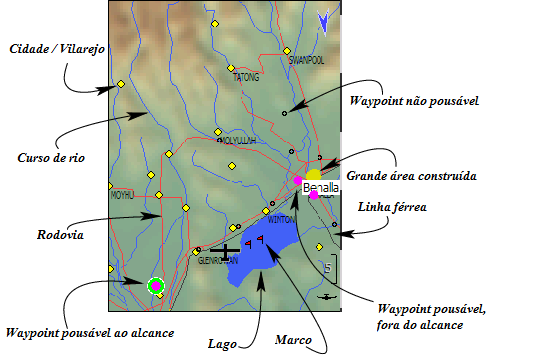
\includegraphics[angle=0,width=0.9\linewidth,keepaspectratio='true']{figures/fig-map.png}
\end{maxipage}

O mapa dinâmico mostra: 
\begin{enumerate} 
\item Aeronave, indicador de vento, perfil da termal, indicador de planeio final
\item Terreno, planícies e planaltos
\item Topografia, rios, rodovias e cidades
\item Waypoints, aeroportos e pousos
\item Prova ativa, zonas de observação e pilões
\item A direção (ou rota\footnote {A linha até o próximo waypoint pode ser uma {\em rota}, como descrição na seção~\ref{sec:route}.}) para a direção para o próximo waypoint.
\item Espaços aéreos
\item Marcadores, histórico de termais, trilha
\item Alcance do planeio\footnote{O alcance do planeio também é citado como
  {\em alcance}, assim como descrito na seção ~\ref{sec:reach}.}
\end{enumerate}
O mapa é desenhado em um sistema de coordenadas projetadas (sem latitude e longitude), e a escala pode ser alterada (zoom + e zoom -), bem como deslocado.  Todas as funções de navegação levam a curvatura da Terra em consideração.

\section{Símbolo do planador, orientação do mapa}
O símbolo do planador mostra a posição da aeronave no mapa.  A orientação da aeronave indica a direção estimada que a aeronave está apontando.

O mapa é orientado de três formas: norte acima, trilha acima e alvo acima.  O ajuste da configuração pode ser utilizado para especificar uma orientação diferente no mapa quando estiver em modo de círculos.  É bem útil para prevenir a desorientação quando olhar o mapa girando.  O modo alvo acima facilita determinar em qual direção se deve sair da termal.

Quando o modo trilha ou alvo acima é usado no modo de círculos, o símbolo da aeronave é centralizado na tela, mesmo que o símbolo seja configurado de outra forma.  No modo de cruzeiro, a orientação de trilha e alvo acima permite que o símbolo da aeronave seja posicionada (ex. 20\%) na parte inferior da tela, fornecendo uma boa visão do mapa à frente da aeronave.  Esta posição é definida nos ajustes da configuração.  

\section{Zoom e escala do mapa}\label{sec:zooming}

Para alterar a escala do mapa, dependendo do hardware, você usa:
\begin{enumerate}
\item Toque/clique em uma parte vazia do mapa para sublinhar o mapa se já não estiver selecionado.  Então utilize a roda do mouse ou as teclas acima/abaixo do Pocket PC para zoom + ou zoom -.
\item Um dispositivo PNA com um botão rotativo permite que se altere o zoom.
\item Dispositivos Android tem o +/- que permite que se altere o zoom.
\item Você pode também fazer o gesto para mudar o nível de zoom. Gesto acima (veja à esquerda) aumento o zoom.  Para baixo diminui o zoom.\gesturespec{up}
\item Ou selecione a função através do menu.
\begin{quote}
\bmenug{Mostrar 1}\blink\bmenug{Zoom In} e \bmenug{Zoom Out}
\end{quote}
\item No Altair, o botão rotativo pode ser usado para alterar o zoom.
\end{enumerate}

A escala do mapa é mostrada no canto inferior do mapa dinâmico.  A distância indicada é medida da borda esquerda para a direita do mapa dinâmico.
Usuários do Compaq Aero:  Se você ativar as teclas de jogo do Compaq Aero (no Menu-Q), os dois botões centrais serão as teclas acima/abaixo.
\marginpar{\includegraphics[angle=0,width=0.4\linewidth,keepaspectratio='true']{figures/zoom.png}}

Usuários do Compaq Aero:  Se você ativar as teclas de jogo do Compaq Aero (no Menu-Q), os dois botões centrais serão as teclas acima/abaixo.

\subsection*{Zoom Girando}
Há uma facilidade de ter dois tipos de zoom: um quando a aeronave está em modo girando e outro em modo de cruzeiro ou modo final.  Esta é a opção de Zoom girando, nos ajustes das configurações.  Por padrão, o zoom girando é ajustado em 2,5 – 5,0km dependendo do tamanho da tela.  Quando o usuário altera o zoom, afeta diretamente o zoom atual somente.  Quando se sai do modo atual de zoom, é usado o modo prévio de zoom. Se o modo de Zoom girando não está ativo, haverá somente um único nível de zoom.  Esta situação conduz a diferentes níveis de zoom sendo preservados para serem alterados manualmente, independentemente dos ajustes de Auto Zoom.
 
\subsection*{Auto Zoom}
Auto Zoom automaticamente aproxima a tela quando se está aproximando de um waypoint para manter a visualização em uma distância apropriada. 
\marginpar{\includegraphics[angle=0,width=0.4\linewidth,keepaspectratio='true']{figures/zoomauto.png}} 
Quando o Auto Zoom está ativo, ‘AUTO’ aparece perto da escala do mapa.

Para ativar o Auto Zoom, use o gesto \gesturespec{ud} ou o menu descrito à esquerda. Para voltar ao zoom normal, faça o zoom manualmente, não importando o que já foi feito por menu ou gesto. 

\menulabel{\bmenug{Mostrar 1}\blink\bmenut{Zoom}{Auto}}
Quando um waypoint muda (automaticamente, através do seletor de prova ou manualmente selecionando waypoints), o Auto Zoom ajusta o nível de zoom automaticamente para que o próximo waypoint seja visível no mapa.

Durante o modo Girando se uma termal foi detectada, o mapa é centrado sobre a termal ou parte dela para que a aeronave continue sendo visível.
 
\section{Navegando no mapa (Panning)}\label{sec:panning}

O modo panorâmico permite ao usuário explorar áreas que estão além da aeronave.  É bem útil quando se está planejando a prova.
\begin{enumerate}
\menulabel{\bmenug{Mostrar 1}\blink\bmenug{Pan On}}
\item Ative o modo panorâmico por menu ou gesto.  O gesto para este modo é mover sua ponta do dedo acima, direita, abaixo e esquerda, formando um “P”. 
\gesturespec{urdl}
\item O mapa pode ser movido arrastando a tela ou usando as teclas.  Para Altair, modo panorâmico é feito com o botão rotativo interno/externo.  
\item Quando feito, o modo panorâmico pode ser desabilitado manualmente, pressionando PAN OFF no sub-menu.
\end{enumerate} 

\sketch{figures/pan.png}
Quando o modo panorâmico está ativo, as letras ‘PAN’ aparecem próximas à escala do mapa.  Enquanto estiver nesse modo, o foco estará na mira no meio do mapa.

Apesar de aparecer a mira (para usuários Altair), o mapa continuará oferecendo a opção “Oque Aqui?” tocando em qualquer posição no mapa (na tela de toque). 


\section{Waypoints} \label{sec:waypoint-schemes}
Os waypoints são mostrados com símbolos diferentes, dependendo do tipo do waypoint; a maior diferença são waypoints pousáveis e não pousáveis.

\subsection*{Pousáveis}
Os símbolos dos waypoints são desenhados conforme abaixo.  Há três conjuntos de ícones disponíveis para waypoints pousáveis. \config{waypointicons}

\begin{tabular}{c|ccc|ccc|}
Conj. Ícones 
&\begin{sideways}Pousável\end{sideways}
&\begin{sideways}Marginal\end{sideways}
&\begin{sideways}Alcançável\end{sideways}
&\begin{sideways}Aeródromo\end{sideways}
&\begin{sideways}Marginal\end{sideways}
&\begin{sideways}Alcançável\end{sideways}\\
\hline
Círculo Roxo &
\includegraphics[width=0.8cm]{icons/winpilot_landable.pdf} &
\includegraphics[width=0.8cm]{icons/winpilot_marginal.pdf} &
\includegraphics[width=0.8cm]{icons/winpilot_reachable.pdf} &
\colorbox{white}{\includegraphics[width=0.8cm]{icons/winpilot_landable.pdf}} &
\includegraphics[width=0.8cm]{icons/winpilot_marginal.pdf} &
\includegraphics[width=0.8cm]{icons/winpilot_reachable.pdf} \\
\hline
Branco e Preto &
\includegraphics[width=0.9cm]{icons/alt_landable_field.pdf} &
\includegraphics[width=0.9cm]{icons/alt_marginal_field.pdf} &
\includegraphics[width=0.9cm]{icons/alt_reachable_field.pdf} &
\colorbox[rgb]{0.94,0.94,0.94}{\includegraphics[width=0.9cm]{icons/alt_landable_airport.pdf}} &
\includegraphics[width=0.9cm]{icons/alt_marginal_airport.pdf} &
\includegraphics[width=0.9cm]{icons/alt_reachable_airport.pdf} \\
\hline
Luzes de tráfego &
\includegraphics[width=0.9cm]{icons/alt2_landable_field.pdf} &
\includegraphics[width=0.9cm]{icons/alt2_marginal_field.pdf} &
\includegraphics[width=0.9cm]{icons/alt_reachable_field.pdf} &
\colorbox{white}{\includegraphics[width=0.9cm]{icons/alt2_landable_airport.pdf}} &
\includegraphics[width=0.9cm]{icons/alt2_marginal_airport.pdf} &
\includegraphics[width=0.9cm]{icons/alt_reachable_airport.pdf} \\
\hline
\end{tabular} \\

Os ícones marginais são desenhados para aqueles waypoints que estão principalmente no alcance, mas não é possível a aproximação direta (ex. uma montanha não permite a aproximação direta).
  
Os waypoints são rotulados opcionalmente de acordo com suas abreviações, esquemas e visibilidade.

No topo dos waypoints pousáveis, pode haver mais detalhamento.  Se houver a opção ativada 
`{\it Detalhar Pousáveis}' você terá informações adicionais quando houver a visualização deste waypoints.

\begin{enumerate}
\item  Campos pousáveis têm ícone quadrado apesar de serem mostrados em tabela.  O quadrado é desenhado como um diamante em pé.  Aeródromos permanecem com um círculo, facilitando sua visualização. 
\item  Todo o conjunto de ícones, incluindo o conjunto de “círculos roxos”, colocam a pista em suas atuais direções.  A direção da pista está disponível nos dados do waypoints.  Ex. os waypoints de formato (\verb|.cup|) não incluem esta informação.
\end{enumerate}

\subsection*{Pousáveis ao Alcance}
Próximo aos pousáveis, há uma estimativa da altitude acima da altura de segurança dos pontos pousáveis e é mostrada próxima ao waypoints.  Esta característica é uma das capacidades mais poderosas do XCSoar.  A altitude de chegada é calculada configurando-se o computador de planeio do XCSoar com parâmetros de polar, ajustes de MacCready, vento, abertura do terreno e altitudes de segurança.  Com tudo isso sendo configurável, há muito espaço para erros, portanto:

A menos que tenha entendido completamente os conceitos de cálculo de planeio, você deve \warning manter a pré-configuração do XCSoar (já julgado e fortemente aprovada).

É da responsabilidade do piloto sempre interpretar a leitura e observar os valores com o tempo.  Todavia, tendo ajustado o computador de planeio seguindo o Capítulo 
\ref{cha:glide} mostra a altitude estimada de alcance, desenhada ao lado de campos pousáveis ao alcance levam em consideração o relevo ou mostram ambos.
\config{arrivalheight}

Outra opção é mostrar o planeio médio necessário para um campo pousável ao alcance.  Este cálculo é derivado da distância atual ao campo pousável dividido pela diferença de altura entre a altura atual e a altura do campo pousável.  Novamente, a altura de segurança é adicionada à altura do campo pousável, mas nada mais é levado em consideração: sem vento, sem polar, sem ajuste MacCready, só geometria.  O conceito do planeio médio necessário é amplamente discutido, como um conceito bem robusto.

\tip Tenha em mente que necessita de um forte conhecimento dos dados de alcance e ajustes no computador de planeio.

\subsection*{Não Pousáveis}
Como o arquivo de waypoints contém informações da natureza do campo não-pousável, o mapa mostrará ícones específicos para estes pontos.  A tabela contém uma relação dos ícones de mapas apresentados (veja figura  \ref{fig:nonlandables}).

\begin{figure}[h]
\centering
\vspace{2.5cm}
\begin{tabular}{ccccccccc}
\begin{rotate}{60}Waypoint simples\end{rotate} &
\begin{rotate}{60}Topo da montanha\end{rotate} &
\begin{rotate}{60}Obstáculo\end{rotate} &
\begin{rotate}{60}Passagem\end{rotate} &
\begin{rotate}{60}Planta ou fábrica\end{rotate} &
\begin{rotate}{60}Torre ou prédio\end{rotate} &
\begin{rotate}{60}Túnel\end{rotate} &
\begin{rotate}{60}Estação metereológica\end{rotate} &
\begin{rotate}{60}Ponte\end{rotate}\\

\includegraphics[width=0.5cm]{icons/map_turnpoint.pdf} &
\includegraphics[width=0.8cm]{icons/map_mountain_top.pdf} &
\includegraphics[width=0.7cm]{icons/map_obstacle.pdf} &
\includegraphics[width=0.7cm]{icons/map_pass.pdf} &
\includegraphics[width=0.8cm]{icons/map_power_plant.pdf} &
\includegraphics[width=0.7cm]{icons/map_tower.pdf} &
\includegraphics[width=0.6cm]{icons/map_tunnel.pdf} &
\includegraphics[width=0.6cm]{icons/map_weather_station.pdf} &
\includegraphics[width=0.8cm]{icons/map_bridge.pdf} \\

\end{tabular}
\caption{não pousáveis}\label{fig:nonlandables}
\end{figure}

\section{Prova ativa}

O curso da prova ativa é desenhado no mapa em linha azul (pontilhada).  As áreas atribuídas às provas mostram os setores dos pilões ou áreas sombreadas em amarelo.  Círculos são desenhados ao redor dos pontos de início e fim, as linhas são desenhadas nos pontos de início e fim se os pontos são deste tipo.  Os setores de observação da prova são desenhados em segmentos de círculos.

A todo tempo, uma linha fina é desenhada da aeronave até o próximo waypoint da prova.  Esta linha deve ser um caminho direto ao waypoint, ou ser uma rota livre de terrenos e espaços aéreos, descritos anteriormente em detalhes na seção
~\ref{sec:route}.

\begin{center}
\begin{tabular}{c c c}
{\it Início/Fim} & {\it Setor} & {\it Cilindro} \\
\includegraphics[angle=0,width=0.3\linewidth,keepaspectratio='true']{figures/cut-startfinish.png} &
\includegraphics[angle=0,width=0.3\linewidth,keepaspectratio='true']{figures/cut-sector.png} &
\includegraphics[angle=0,width=0.3\linewidth,keepaspectratio='true']{figures/cut-barrel.png} \\
\end{tabular}
\end{center}


\section{Terreno e Topografia}\label{sec:terrain_topo}

As seguintes características de topografia são desenhadas no mapa:
\begin{itemize}
\item Rodovias principais, mostradas em linhas vermelhas
\item Rios, mostrados em linhas azuis
\item Grandes corpos de água (lagos), mostrados em áreas azuis
\item Cidades grandes, mostradas em áreas amarelas
\item Áreas de pequena população, mostrada como diamantes amarelos 
\end{itemize}
Cidades e pequenas áreas com população são rotuladas em itálico.

O solo é colorido de acordo com a elevação e opcionalmente sombreado pelo sol ou pela direção do vento.  Solos inválidos ou abaixo do nível do mar são coloridos em azul.


\menulabel{\bmenug{Mostrar 2}\blink\bmenut{Terreno}{On/Off}}
\menulabel{\vspace{1cm}\bmenug{Mostrar 2}\blink\bmenut{Topo.}{On/Off}}

O solo é sombreado para melhorar a visibilidade.  O sombreamento padrão é ajustado coincidindo a iluminação virtual com a direção do vento, sendo as áreas mais brilhantes são barlavento e as áreas mais escuras são sotavento.   
A inclinação solar também foi implementada.  Se o sombreamento da encosta for ajustado para ‘Sol’, o brilho da encosta segue conforme o dia e hora.  A quantidade de sombra sobre o brilho do terreno é ajustável \config{shading}.

A visualização do solo e topografia podem ser acionados ou não através do menu.

\begin{tabular}{c c}
Topografia & Terreno \\
\includegraphics[angle=0,width=0.4\linewidth,keepaspectratio='true']{figures/cut-topo.png} &
\includegraphics[angle=0,width=0.4\linewidth,keepaspectratio='true']{figures/cut-terrain.png} \\
\end{tabular}

Se os dados do solo não estiverem disponíveis (ou a visualização estiver desligada), a cor de fundo do mapa será branca.  Todo o solo abaixo do nível médio do mar é mostrado em azul.  Se você estiver voando fora da terra, o fundo da tela será branco.  

\subsection*{Rótulos do mapa}\label{sec:maplabels}

A tela pode ser mais clara desligando a visualização dos rótulos de topografia e waypoints for a da prova escolhendo o menu ‘Rótulos’.
\menulabel{\bmenug{Mostrar 2}\blink\bmenut{Rótulos}{Nenhum}}

Outra opção para deixar mais clara incluem:

\jindent{\bmenuth{Rótulos}{Prova \&}{locais pouso}}{  Mostra rótulos para os waypoints na prova ativa e campos pousáveis (baseado nos atributos dos waypoints).  Os outros waypoints serão mostrados, mas sem rótulos. }

\jindent{\bmenut{Rótulos}{Prova}}{ Mostra somente os rótulos dos waypoints da prova ativa.}
\jindent{\bmenut{Rótulos}{Todos}}{ Mostra todos os rótulos para todos os waypoints.}

Note que em todos os casos, a formatação dos rótulos é configurável no menu
`{\it Waypoint Display}'.  \config{labels}


\section{Rastro}\label{sec:trail}


Um rastro opcional pode ser desenhado no mapa dinâmico para mostrar o caminho da aeronave.  A cor e a espessura do rastro dependem de altitude ou do valor do variômetro.


\begin{center}
\includegraphics[angle=0,width=0.5\linewidth,keepaspectratio='true']{figures/snail.pdf}
\end{center}

Se houver conexão do Vega ou outro variômetro inteligente com a saída Netto, o valor do vário Netto é usado; conseqüentemente as cores e a espessura do rastro indicarão o movimento vertical da massa de ar ao invés do movimento vertical da aeronave.

\config{snailtrail}
A visualização do rastro pode ser ajustada entre Desligado, Curto (+/- 10 minutos), Longo (+/- uma hora) ou Completo que mostrará todo o vôo.  Isto pode ser ajustado através dos ajustes de configuração ou temporariamente através do menu.
\menulabel{\bmenug{Mostrar 2}\blink\bmenut{Trilha}{Completo}}

Observe que para todos estes modos, o rastro é curto no modo Girando para facilitar a visualização.

De modo a auxiliar a centralização das térmicas na presença de vento, o rastro pode ser artificialmente derivado com o vento conforme vai sendo mostrado (é a compensação de deriva).  Deste modo, o rastro é referenciado pelo vento e não pelo solo.  Assim como as termais também são derivadas com o vento, o rastro pode dar uma indicação mais precisa onde esteve a aeronave com relação às termais.

O exemplo é ilustrado abaixo.  Observe que, quando a compensação da deriva do vento está ativa (figura à direita), a aeronave aparenta estar girando em uma coluna ao invés de estar em uma espiral alongada (figura à esquerda).

\begin{center}
\includegraphics[angle=0,width=0.6\linewidth,keepaspectratio='true']{figures/traildrift.png}
\end{center}

\config{traildrift}
Ativando a compensação da deriva do rastro é através dos ajustes de no menu de configuração. A compensação só é feita no modo Girando; a visualização do rastro no modo Cruzeiro não é afetada.  Também pode ser alterada pela janela de ajuste do vento.
\menulabel{\bmenug{Config 1}\blink\bmenus{Vento}}

A visualização do rastro é útil também para mostrar mais claramente quando as termais são cisalhadas pelo vento.
A largura da trilha pode ser opcionalmente alterada de acordo com a visualização do variômetro.  


\section{Marcadores}\label{sec:markers}

Os marcadores são mostrados como pequenas bandeiras no mapa.  Os marcadores podem ser adicionados manualmente ou automaticamente.  Um exemplo de como estes marcadores podem ser adicionados automaticamente é quando se entra em modo Girando, um modo simples de mostrar as termais encontradas.

\menulabel{\bmenug{Nav 2}\blink\bmenut{Marca}{Ponto}}
Os marcadores não são mantidos após o XCSoar ser fechado, porém a localização dos marcadores é anexada ao arquivo
 \verb|xcsoar-marks.txt|.

\section{Termais}

Enquanto estiver girando em termais, automaticamente será gerado um marcador e mantido até o \sketch{figures/thermalhistory.png} fim do vôo.  Este histórico termal é acessível através da função de elementos de mapa, da mesma forma que os marcadores ou waypoints.


\section{Linha de alcance de planeio}\label{sec:reach}

Uma linha de alcance de planeio é mostrada no mapa como uma linha pontilhada branca e preta, indicando onde a aeronave poderá pousar em terreno aberto.  O alcance é mostrado em todas as direções, incluindo caminhos obstruídos no terreno.  Esta opção é útil para conhecer o planeio relativo à topografia quando se está baixo e procura por termais, ou quando está voando em áreas montanhosas.

Os cálculos para o alcance podem ser configurados \config{turningreach} em dois níveis: 
\begin{description}
\item[Linha reta] se o alcance em curva está desabilitado, mostrará a maior distância que a aeronave pode voar no planeio final em todas as direções sem fazer curvas.  O alcance aparece como um anel fechado ao redor da aeronave.  

\begin{center}
\includegraphics[angle=0,width=0.8\linewidth,keepaspectratio='true']{figures/reach1.png}
% CUTOUT SHOWING GLIDE RANGE FOOTPRINT.  NO TOPOGRAPHY, FULLSCREEN, NO TASK. TURNING=FALSE
\end{center}

\item[Girando] se o modo Girando estiver ativo, o planeio será mostrado como a maior área que a aeronave pode alcançar em todas as direções, mesmo permitindo curvas ao redor de obstáculos.  A área de alcance aparece com um anel fechado ao redor da aeronave mas também pode incluir buracos indicando picos de montanhas que a aeronave não pode alcançar sem subir.

\begin{center}
\includegraphics[angle=0,width=0.8\linewidth,keepaspectratio='true']{figures/reach2.png}
% CUTOUT SHOWING GLIDE RANGE FOOTPRINT.  NO TOPOGRAPHY, FULLSCREEN, NO TASK. TURNING=TRUE
\end{center}

\end{description}

A tela pode ser configurada também para desfocar as áreas não alcançáveis fora do alcance do planeio da aeronave.  O caminho do planeio final é verificado levando-se em consideração também a abertura do terreno através do caminho e também a altura do terreno.
Se a abertura (clareza) do terreno não é atingida, aparecerá uma cruz vermelha no mapa onde a área é perigosa.  Se um alvo for definido, os cálculos são feitos através do caminho reto para o alvo.  Se não há alvo definido, o cálculo é feito através do caminho que está seguindo.
Se o alcance estiver ativo, o modo de aborto de prova usará os waypoints pousáveis e abrirá uma lista também com os waypoints alternativos do mapa.
Observe que os cálculos da prova não são afetados pelos cálculos de alcance – por exemplo, não são levados em conta os dados de altitude necessária para finalizar a prova e dados mostrados nas infoboxes.

Além do mais, os cálculos são usados para o anel de alcance, altura de chegada para waypoints pousáveis, modo de aborto e janelas de diálogo alternativas.  O desempenho da aeronave e os ajustes de MacCready usados nestes cálculos são configuráveis\config{reachpolar}:
\begin{description}
\item[Prova] O valor de MC é o usado na prova.
\item[Safety MC] Um valor de MC baixo pode ser configurado para ser usado como referencial ao melhor planeio da aeronave.  O grau de segurança alcançado nos cálculos é feito com a diferença entre o melhor desempenho de planeio e o planeio seguindo o MacCready de Segurança (speed to fly).  
\end{description}

\section{Abas de estado `{\it Voo}' e `{\it Tempo}'}\label{sec:flight-status}

A janela de diálogo Estado é multi-tabular, fornecendo uma visão geral da informação do vôo, sistema, prova, regras e tempos.  Pode ser acessada com o gesto “S” ou com o botão do Menu. 
\gesture{Esquerda - Baixo - Direita - Baixo - Esquerda}
\begin{quote}
\bmenug{Info 2}\blink\bmenug{Estado}
\end{quote}

\subsection*{Vôo}
Selecione a página `{\it Flight}'. 
A janela mostra a localização da aeronave e pode ser útil quando se reporta a posição.  Mostra a posição da aeronave, o máximo ganho de altura, waypoints mais próximo, ângulo de direção e distância.
\sketch{figures/status-flight.png}

Você pode achar esta função útil quando for reportar sua localização para outros pilotos ou resgate.

\subsection*{Tempo}\label{sec:time-status}
Seleciona a aba  `{\it Times}'. 
Mostrará a hora local, tempo de vôo, hora da decolagem e pouso e hora do nascer e pôr do sol.

Observe que estes valores nesta aba são estáticos e só serão atualizados a cada abertura de aba. 
\sketch{figures/status-times.png}
Para ver os dados atualizados, é necessário fechar a aba e abrí-la novamente.  Os valores serão atualizados automaticamente a cada abertura desta janela.  Familiarize com este procedimento antes de realizá-lo em vôo.


\section{Rota}\label{sec:route}

O XCSoar pode planejar caminhos pelo terreno e obstáculos no espaço aéreo em três dimensões da aeronave até o destino.  Este caminho é conhecido como rota.  A altura do destino é a altura de chegada para waypoints finais ou pode ser mais alto para waypoints intermediários, se forem regras da prova ou requisitos para completar a prova.  

As funções de planejamento de rota são ordenadas por modo de prova, modo de aborto e modo ‘ir para’.

\begin{center}
\includegraphics[angle=0,width=0.8\linewidth,keepaspectratio='true']{figures/route3.png}
\end{center}

As rotas levam em consideração o desempenho da polar e são calculadas para levarem o mínimo tempo.  Por padrão, os cálculos de rota são desativados e podem ser ativados somente por solo ou quando na prevenção de espaço aéreo. \config{routemode}

O solo é evitado verticalmente pela altura de segurança do terreno \config{safetyterrain}, sem nenhuma abertura de terreno lateral.  As rotas válidas podem  resultar na chegada da aeronave ao destino mais alta que a altura mínima – como pode ocorrer quando o destino está além de uma montanha mais alta.

O espaço aéreo é evitado horizontalmente por uma margem de aproximadamente 250m sem nenhuma abertura imposta verticalmente.  As rotas válidas podem voar acima ou abaixo do espaço aéreo.

Se o MacCready é positivo, a subida é opcionalmente permitida nos cálculos de rota.  O topo da subida deve ser limitado a 500m acima do teto de início e final, ou incluso no teto, definido pelo teto da termal \config{routeceiling}.  As subidas acima da altitude de início e final são penalizadas por uma taxa de subida mais lenta que o valor de MacCready atual.

Algumas aproximações e limitações do sistema de planejamento de rotas são:
\begin{itemize}
\item Quando subidas são necessárias (e permitidas) para alcançar o destino, as subidas podem ocorrer no início da rota. 
\item Segmentos de subidas em cruzeiro podem ocorrer em altitude constante, equivalente a muitas pequenas subidas distribuídas ao longo do caminho. 
\item Falhas sobre o resultado dos cálculos podem se reverter em vôo direto da aeronave, de sua localização atual para o destino.
\end{itemize}



%%%%%%%%%%%%%%%%%%%%%%
% !TeX encoding = utf8
% !TeX spellcheck = en

\chapter{Cross Country Tasks}\label{cha:tasks}

XCSoar provides a full task management system, in which tasks can be
edited prior to flight and, when undertaking casual cross-country
flying, modified during flight.  Waypoints are advanced automatically
or may be cycled through manually. Many of XCSoar's computations relate to
either turnpoints or the finish waypoint.
Unless a ``true'' task is defined, XCSoar will provide a ``go home'' function, with
many of the task related functions referring to the location of takeoff.
This chapter also describes the use of IGC loggers with XCSoar.

There are three task modes available:
\begin{description}
\item[Ordered task] This is the natural cross-country task type,
in which the task consists of a start point, zero or more waypoints,
and a finish point.  The task points are to be flown in order.
\item[Goto task] Flight to a single destination.
\item[Abort task] Provides options to fly to the nearest landing points.
\end{description}

Note that in goto and abort modes, the ordered task is retained and may be resumed
later, preserving any statistics about achievement in the task.

\subsection*{Automatic goto}

If no ordered task is defined, then on takeoff, a goto task is automatically
established with the takeoff point as the destination, or the nearest airfield
if it was close to the takeoff point.

Whether or not a task is defined, the takeoff point is always
generated and appears in the waypoint list for later reference or use.

After having defined an ordered task for the very first time, the automatic ``goto takeoff'' function is skipped. To resume a simple task, use goto.

\section{Goto tasks}

Goto tasks may be established by selecting a waypoint from the map,
the waypoint list, or any other mechanism e.g.\ the alternates dialogue,
and select \bmenuw{GoTo}. In goto task mode, selecting
\bmenug{Nav 2}\blink\bmenug{Task Resume} resumes the ordered task (if
any).

\section{Editing tasks}

You can edit tasks in several ways.  Some methods are more useful for
editing prior to flight, and others allow tasks to be modified whilst
in flight for casual cross-country touring.  Tasks can be saved to
files and reloaded later, and can be transferred between any XCSoar
platform (Android, Windows, Linux\textellipsis).

\tip{} It is also possible to save a `default' task and have this task loaded
automatically upon start-up of XCSoar.  One application of this is to
set up a default task with one waypoint being the home --- this means
that XCSoar is then programmed for final glide back to home, which is
useful for casual cross-country touring.

The main ways of setting tasks are the following:
\begin{itemize}
\item Using the task editor dialogue
\item Selecting waypoints from the map and adding them to the task from the
 waypoint details dialogue
\item Loading the task from a file
\end{itemize}

%Selecting the Task menu item will produce the Task dialogue box.  The
%list box on the left displays all of the turn points loaded into the
%system. Highlight the desired entries and using the ``-$>$'' and ``$<$-''
%buttons assemble the desired task in the Task list box. As each turn
%point is added to the task a continuous display of the calculated task
%length is shown.  Tasks can be saved for recalling later using the
%``Save'' button and recalled using the ``Load'' button.  Once the desired
%task is complete select ``OK''.
%
%{\it DIAGRAM SHOWING TASK DIALOG EDITING, WITH LABELED ARROWS POINTING
%TO THE USER INTERFACE ELEMENTS?}

Loading a task from file may be useful in competition or casual
cross-country flying in groups, as one person can distribute the task
file to others, thereby saving effort on editing the task severalfold.
\tip{}
If no task is present at startup, a task is created automatically,
containing one waypoint takeoff as ``goto home''.

XCSoar saves the current task when shutting down and loads it at
startup, thereby allowing the task to be entered early in the day,
then the device running XCSoar can be turned off until flight time.

Task waypoints are preserved even if the waypoint
file is changed.  This means, if you save a task, then change the
waypoint file, then load the task again, new waypoints are generated
for any waypoints that are missing in the new waypoint file.

\section{Waypoint Information}
%Several ways of selecting a waypoint are available:
%\begin{itemize}
%\item Touch its name or the waypoint symbol on the map screen if it is visible.
%\item If the waypoint is in the active task, highlight the waypoint {\InfoBox}, 
%  then use the up/down arrow keys to select the desired waypoint, and press the
%enter key.
%\item From the Task dialogue, find and highlight the waypoint in
% the waypoint list, then press the 'Details' button.
%\end{itemize}
%The display will now show the waypoint details dialogue.

The waypoint info dialogue describes a waypoint in detail and has
navigation functions such as GoTo, insert, append to the task, or set the 
waypoint as the new home.
This may be accessed in several ways:

\gesturespec{rd}or menu \bmenug{Nav 1/2}\blink\bmenug{Task},
\todonum{descr.\ tabular ``Turn Points''}
highlight a waypoint, then tap the highlighted waypoint again to display the 
task point dialogue, then push \bmenuw{Details}.

\gesturespec{dl}or menu \bmenug{Nav 1/2}\blink\bmenug{Alternates}
to show the
details of the landables nearest to the aircraft.

\gesturespec{dr}or menu \bmenug{Nav 1/2}\blink\bmenug{Waypoint List}
, highlight and \bmenuw{select} a waypoint to show its details.

\gesturespec{urdl}or menu \bmenug{Display 1/2}\blink\bmenug{Pan On} to put the 
map into pan mode, pan to the desired waypoint, touch its name or the waypoint 
symbol.

\bmenug{Info 1/3}\blink\bmenug{What's here?}
to show the
item list under the cross-hair, or your index finger on the map.

The waypoint details dialogue contains two major pages (accessed via the
\bmenuw{$>$} and \bmenuw{$<$} buttons). Depending on the availability of further
details of the waypoint they will by shown on extra pages.

\subsection*{Waypoint details}\label{sec:waypointdetails}
This page contains text giving the name of the waypoint,
the waypoint's GPS coordinates, elevation, radio frequency and 
runway information (if this information is in the waypoint file), 
local daylight time, bearing and distance to the waypoint, and the altitude 
differences required 
to reach the waypoint as described below. In addition, there is a button 
\bmenuw{GoTo} to directly initiate
navigating to this waypoint. The button cancels the current task. 
\begin{center}
\includegraphics[angle=0,width=0.8\linewidth,keepaspectratio='true']{figures/dialog-waypointdetails0.png}
\end{center}

As mentioned above, the Waypoint info dialogue also shows three forms of altitude 
difference (additional
altitude required to reach the waypoint at the safety height) for
the corresponding waypoint:
\begin{description}
\item[Alt diff MC 0] Altitude difference at MC setting of~0
\item[Alt diff MC safety] Altitude difference at the abort/safety MacCready 
  setting (see~\ref{sec:safety-factor})
\item[Alt diff MC current] Altitude difference at the current MacCready setting
\end{description}

From the main Waypoint Info screen, you can access the second page by using the 
\bmenuw{$>$} and \bmenuw{$<$} buttons in the bottom left corner of the page.
Depending of the type and number of details available for a waypoint,
other pages could be available.

\subsection*{Task actions menu}  
This page contains a column of buttons allowing various actions to be performed:
\begin{description}
\item[\button{Replace in task}] replaces the active waypoint in the task with 
  the selected waypoint.
\item[\button{Insert in task}] inserts the selected waypoint before the active 
  waypoint in the task.
\item[\button{Append to task}] adds the selected waypoint to the end of the task.
\item[\button{Remove from task}] removes the selected waypoint from the task.  
  Note that this option is only visible if the selected waypoint is included in 
  the active task.
\item[\button{Set as new home}] sets the waypoint as the home airfield.
\item[\button{Pan to waypoint}] switches to pan mode and pans to that waypoint.
\item[\button{Set Active Frequency}] %TODO To define
\item[\button{Set Standby Frequency}] %TODO To define
\item[\button{Edit}] allows to change the various attributes of the selected waypoint
\end{description}

It is a good idea to set your home waypoint from the waypoint details
dialogue. This causes XCSoar to start up at the home location regardless
of whether a GPS fix is received.  If no home is set, then XCSoar
starts in the centre of the terrain map.

\subsection*{Airfield information}
This page may contain relevant text from the en-route supplement about
the airfield, including runways, radio frequencies, traffic patterns,
contacts.
See Section~\ref{sec:airfield-details}.
\begin{center}
\includegraphics[angle=0,width=0.8\linewidth,keepaspectratio='true']{figures/dialog-waypointdetails1.png}
\end{center}

\subsection*{Waypoint details image}
This page shows a satellite image of the waypoint.

\begin{center}
\includegraphics[angle=0,width=0.8\linewidth,keepaspectratio='true']{figures/dialog-waypointdetails2.pdf}
\end{center}
How to set up the detailed waypoint information read Section~\ref{sec:airfield-details}.

\section{Waypoint selector dialogue}\label{sec:waypoint-selector-dialog}

The waypoint selector is a dialogue that allows waypoints to be easily selected
from a potentially large database. \gesturespec{dr}

Invoking the selector brings up a filtering dialogue screen with a set of 
\menulabelr{\bmenug{Nav 1/2}\blink\bmenug{Waypoint List}}
optional filters on the left side of the page, and a list of waypoints on the
right, matching all of the filtering conditions set.
There are several filters available, which may be used together,
individually or not at all.
\begin{description}
\item[Name] Selects waypoints, starting with the string typed.
\item[Distance] Filters out waypoints farther than a specified distance from the 
  aircraft.
\item[Direction] Filters out waypoints that are not in a specified direction 
  from the aircraft. 
  An additional special direction ``HDG(xx°)'' (``HDG'' stands for ``heading'') filters waypoints within 30
  degrees to either side of the heading of the glider.  This allows the pilot 
  to point the glider at a group of waypoints and quickly find them.
\item[Type] Filters out waypoints that are not of the specified type
(Landable point, Airport, Turnpoint, etc.) or that appear in the specified File~1 or
File~2 (primary or secondary waypoint file respectively), or in recently-used files.
\end{description}
When filtering by name and type, the list of matching waypoints is
sorted by name. When (in addition) filtering by distance or direction,
 the list of matching waypoints is sorted by distance.

\begin{center}
\includegraphics[angle=0,width=0.8\linewidth,keepaspectratio='true']{figures/dialog-waypointselect.png}
\end{center}

The list can be scrolled if there is more than one screen full of
matching waypoints.  To scroll through the list, simply drag with the finger, or
move to the bottom (or top) of the list with the cursor.   

Selecting an item will result in different behaviour
depending on what function opened the waypoint selector.  In typical
use it brings up the waypoint details dialogue for the selected
waypoint.

\section{Task manager}\label{sec:task-manager-dialog}
\gesturespec{rd}

The task manager is used to edit, view, load, save to file, and declare cross
country tasks.
\menulabelr{\bmenug{Nav 1/2}\blink\bmenug{Task}}

The primary page is a calculator. It shows various calculations 
related to the active task, as described in detail below.  In addition, there 
are buttons for invoking dialogues \bmenuw{Turn Points}, \bmenuw{Manage}, 
and \bmenuw{Rules}, as well as a button to \bmenuw{Close} the task manager.

\subsection*{Task calculator dialog}\label{sec:task-calc-dial}
The task calculator dialogue allows the pilot to see the effect of
various changes to the task on final performance.
\menulabelr{\bmenuw{Calculator}}

In flight the Task Calculator might also be accessed from the Analysis pages. 
With pages Task, Climb, and Task Speed a button \bmenuw{Task Calc} comes up,
that directly changes to the Task Calculator screen.


\begin{center}
\includegraphics[angle=0,width=0.8\linewidth,keepaspectratio='true']{figures/dialog-taskcalculator.png}
\end{center}

\begin{description}
\item[Estimated task time]  This field displays the estimated total time 
  on task to complete the task at the provided MacCready setting.
\item[Remaining task time]  This field displays the time remaining to complete the task.
\item[Task distance]  This field displays the total task distance.
\item[Remaining distance]  This field displays the remaining distance to complete the task.
\item[Speed estimated]  This field displays the estimated speed  for the remaining of the task considering the provided MacCready setting.
\item[Speed average]  %TODO: To define
\item[Set MacCready]  Allows the user to adjust the MacCready value and 
  see the effect it has on the estimated task time.
\item[AAT range]  Allows the user to adjust the targets within the remaining 
  AAT areas, to see the effect it has on estimated task time and task distance.
\item[Speed remaining]  This field displays the estimated speed for the
  remainder of the task at the provided MacCready setting.
\item[Achieved MacCready]  This field displays the achieved MacCready value.
\item[Achieved speed]  This field displays the achieved speed %TODO at the achieved MacCready setting???
\item[Cruise efficiency]  100~\% indicates perfect MacCready performance, greater 
than 100~\% indicates better than MacCready performance is achieved through flying
in streets. Less than 100~\% is appropriate if you fly considerably off-track. This 
value estimates your cruise efficiency according to the current flight history 
with the set MC value. Calculation begins after task is started.
\end{description}
See Section~\ref{sec:task-speed-estim} for more details on task speed
and achieved MacCready calculations.

On closing the dialogue the entered MacCready value is used as the MacCready 
setting. If the \bmenuw{Cancel} button is pushed, the MacCready setting is 
unaffected.

The \bmenuw{Target} button, for AAT tasks, adjusts the range
(increases or decreases) so that the estimated task time exceeds the
assigned task time by less than five minutes.  The range is adjusted
target-wise. In typical use, all targets are set to ``auto'' that means the pilot
does not have to manually adjust the range to find the course for arrival at 
the assigned task time, thereby reducing pilot workload.

\subsection*{Turn Points}
This page displays an ordered list of the points in the current active task.
\menulabelr{\bmenuw{Turn Points}} 
If there are no waypoints in the active task, there 
will be only an option to ``Add Turnpoint.''  By highlighting (tapping) the
``Add Turnpoint'' function, then tapping in the highlighted region, the waypoint
selector is displayed, as described above.  Highlighting a waypoint from the 
list and then tapping on the highlighted region adds the waypoint to the task.

\subsection*{Manage}
This page allows for invoking all operations needed to create new or manage 
\menulabelr{\bmenuw{Manage}}already defined tasks.


\begin{itemize}
\item [\bmenuw{New Task}] Clears the current task and resets the task rules to 
  the default values.
\item [\bmenuw{Declare}] If an external logger is connected, this will allow 
  uploading the  active task to the logger and declaring it.
\item [\bmenuw{Browse}] Displays a list of all the saved tasks, allowing the 
  pilot to load a previously saved task.  Note that this option will overwrite 
  the current active task.
\item [\bmenuw{Save}] Saves the current active task.  Upon tapping the 
  \bmenuw{Save} button the pilot will be prompted to enter a file name for the 
  task to be saved.
\end{itemize}

\subsection*{Rules}
The values in the menu depend on the task type selected. Clicking any existing 
\menulabelr{\bmenuw{Rules}} value will bring up another menu allowing the pilot to select a 
different value for this rule.  Task types are discussed in more detail below.

Also, tapping on the \bmenuw{Rules} button again after it is highlighted allows 
toggling between a ``thumbnail'' view of the task map and a larger view of the task.

\section{Task types}
XCSoar currently defines three different task types: Racing, AAT, and FAI badges/records.

A brief description of the task types is included below, but this manual does 
not intend to rephrase FAI rules or contest task types. The reader is encouraged 
to become thoroughly familiar with each task type by referring to contest rules 
or FAI rules, which are available at \url{http://www.fai.org}. 


\subsection*{Racing}
(also known as an ``assigned task'').  The racing task involves flight
around each specified turnpoint in the specified order.  Selecting the racing task 
type allows the pilot to enter the following parameters
(note that if the option
``FAI start/arrival tasks'' is ``On'', only part of these options is available)~:
  \begin{description}
  \item [Arm start manually] If set to ``On'', some extra buttons are presented 
  in order to let you \bmenug{Arm start} as well as \bmenug{Disarm start} in 
  menu \bmenug{Nav 1/2}, controlling  the detection of the start condition.
  \item [Start open time] This is the time when the start zone opens.
  \item [Start close time] This is the time when the start zone closes.
  \item [Start max.\ speed] This is the maximum speed allowed in the start observation
    zone.  This should be set to~0 if there is no limit.
  \item [Start max.\ height] This is the maximum height above the start height
    reference (AGL or MSL) at which a task can be started.  This  should be set to~0
    for no limit.
  \item [Start height ref.] This specifies whether the maximum start height is 
    referenced to ground level of the start point (``AGL'') or Mean Sea Level (``MSL'')
  \item [Finish min.\ height] This is the minimum height based on the finish
    reference (AGL or MSL) at which a task can be finished.  This should be set
    to~0 for no limit.
  \item [Finish height ref.] This specifies whether the minimum finish height 
    is referenced to ground level of the finish point (``AGL'') or Mean Sea Level (``MSL'')
  \end{description}

\subsection*{Assigned area task (AAT) and Modified area task (MAT)}
(also known as ``Turn Area Task'', or TAT).  This is a task through assigned
areas (restricted to cylinder or sector observation zones).  A minimum task time 
applies.  
Rules options for this task type include:
  \begin{description}
  \item [AAT min.\ time]  This is the required minimum time for the task.  Refer
    to contest rules or consult an expert for penalties associated with finishing 
    prior to the minimum time.
  \item [Other rules] All other rules stay the same as in case of task type 
    ``racing''.
  \end{description}


\subsection*{FAI badges/records}
The selection of this type of task allows to define the value of the following field: 
  \begin{description}
  \item [FAI start/finish rules] If set to ``On'', only the type of start, and the start and end times might be set. 
  If set to ``Off'', all other racing task rules might be altered from the FAI standard.
  \end{description}

Once the appropriate task type has been selected and start and finish rules 
have been defined as described above, it is necessary to define the properties 
of each waypoint in the task.  

Once selected, waypoints can be moved with the Up and Down arrows.
The first waypoing is automatically set as a start point, and the last as an arrival point.

\section{Turn Points' task rules}\label{sec:task-rules}

The \bmenuw{Turn Points} dialogue brings up the list of waypoints in the task. 
\menulabelr{\bmenuw{Turn Points}} If no waypoint is already defined, this screen 
will show an empty list. With \bmenuw{(add Turnpoint)}, up and down arrows, and 
\bmenuw{Make Finish} an ordered list of waypoints is created. 
Waypoints can be start point, turnpoint, or finish point.
Highlighting any waypoint on the list and either tapping it again or 
touching the \bmenuw{Edit Point} button brings up the waypoint definition. 
Touching \bmenuw{Change type} will bring up a menu of the various task point 
types available.  Definitions of each point type are given below.

A variety of task rules may be used when specifying tasks, including
the common FAI triangles and Assigned Area Tasks (AAT).  Many aspects
of the rules can also be customised.

Starting and finishing lines are centred on their associated waypoint
and aligned perpendicular to the next and previous waypoints
respectively.

Sector turn-points are 90-degree segments aligned to the bisection of
the previous and next waypoints, as commonly used in FAI tasks.
There is also support for British BGA, and German DAeC sectors.

\subsection*{Start point types}
The conditions to be met for a valid start depend on the type of start:
\begin{description}
\item[Start Cylinder] When the glider leaves the cylinder area.
\item[Start Line] When the glider crosses the start line.
\end{description}

\subsection*{Turnpoint types}
The conditions to be met for a valid turnpoint pass depend on its
 type:
\begin{description}
\item[FAI Sector] When the glider has entered the observation zone (OZ), defined 
by a segment and radial distance from the waypoint.  The segment is
defined by a 90-degree arc centred about the bisector of inbound and
outbound legs, with a distance of 20~km.
\item[Keyhole Sector (DAeC 0.5/10 sector)] When the glider has entered the
observation zone, defined by a segment and radial distance from the waypoint.  The segment is
defined by a 90~degree arc centred about the bisector of inbound and
outbound legs, with a distance of 10~km.  The observation zone also includes
a cylinder of 500~m.
\item[BGA Fixed Course Sector]  When the glider has entered the
observation zone defined by a segment and radial distance from the
waypoint. The segment is defined by a 90-degree arc centred about the
bisector of inbound and outbound legs, with a distance of 20~km.
The observation zone also includes a cylinder of 500~m (British rules).
\item[BGA Enhanced Option Fixed Course Sector]  When the glider has entered the
observation zone defined by a segment and radial distance from the
waypoint. The segment is defined by a 180-degree arc centred about the
bisector of inbound and outbound legs, with a distance of 10~km.
The observation zone also includes a cylinder of 500~m (British rules).
\item[Turnpoint Cylinder]  When the glider has entered the observation zone
defined by a radial distance from the waypoint.
\item[Symmetric quadrant] A symmetric quadrant with a custom radius.
\item[Area Cylinder (AAT)] %TODO To define
\item[Area Sector (AAT)]  When the glider has entered the observation zone
defined by the radial distance from the waypoint, and segment for sector areas.
\end{description}

\subsection*{Finish point types}
Task completion depends on the finish type:
\begin{description}
\item[FAI finish quadrant] A 90~degree sector with a radius of one kilometer. Cross edge to finish.
\item[Finish line] When the glider crosses the finish line.
\item[Finish cylinder] When the glider enters the cylinder area.
\end{description}

Automatic advancement is triggered whenever a condition is met. To start an AAT,
mixed task, or Racing task the start has to be armed before. 

\tip{} Competition rules may be defined in a profile file for
distribution to a group of pilots or task-setters, so all competitors
are playing by the same rules!

Additional task rules for valid starts and finishes may also be
specified.  Starts may have a defined maximum altitude above ground,
and a maximum speed.  Finishes may have a minimum altitude above
ground.  These parameters are defined in the page ``Default Task Rules'' in
the configuration \config{taskrules} settings in 
\bmenug{Config. 1/3}\blink\bmenug{System} in the panels ``Task Defaults/Task Rules'' and ``Task Defaults/Turnpoint Types''.
For non-AAT tasks, an option is available to set the minimum finish
altitude according to the FAI rule, whereby the minimum finish
altitude is above 1000~meters below the start altitude.


\section{Start a task}\label{sec:start-task}
One the waypoints (start, turn points with their special features, finish) and task rules defined, there are two things to do:
\begin{itemize}
\item In the panel ``Manage'', press on \button{Save} to save the task by giving it a name. If you have just modified an existing task, you can either give it the same or give it another name (to create a new task based on an already-existing one).
\item Press on the item \button{Close} of the task manager.
After the creations and changes done, the displayed windows may differ.
You can choose between \button{Close} to use the task you have just modified or created.
The button \button{Revert Changes} allows to discard the changes and continue with the task that was previously loaded.
If you have created and saved a new task, it will not be most: you could find it later on in you list of saved tasks.
However, the activated task would have been erased from the working memory.
You will have to reload the task that you wish to do.
\end{itemize}
Si you push on \button{Close}, the task is started (activated).

\section{Advancing and restarting tasks}\label{sec:advanc-rest-tasks}
At all times one waypoint in the task is designated as the active
waypoint.  The active waypoint is used for calculation and display of
navigation information, that is, the pilot is directed to fly towards
the active waypoint (also referred to as the ``next waypoint'' in the
description of InfoBoxes as in Chapter~\ref{cha:infobox}).

During flight a continuous display of the bearing to the next waypoint is shown.

The altitude required to complete the task is calculated for the route starting
from the glider's actual position going through the task's turnpoints to the 
final waypoint.

Changing the active waypoint is performed automatically, or may be performed manually.
The start point of racing tasks, and AAT task points, are special cases that require
the task point to be ``armed'' before the system will automatically advance to the next
task point once that point is reached.  All other task points will automatically
advance to the next point as soon as the last point was reached.

For non-racing tasks, no user interaction is required to
advance through the task --- the system will automatically advance as
each task point is achieved.  The user may still manually advance or retreat the active
task point by selecting the menu items \bmenug{Nav}\blink\bmenug{Previous turnpoint} and
\bmenug{Nav}\blink\bmenug{Next turnpoint} respectively.

The menu items \bmenug{Previous turnpoint} and
\bmenug{Next turnpoint} show dynamic labels that
indicate the action that will be performed upon selecting the item.

For task points requiring arming, \bmenug{Next Turnpoint} becomes 
\bmenug{Arm turn} if the turn is not armed; if it is armed, then it becomes 
\bmenug{Next Turnpoint} allowing for manual advance. 
\bmenug{Previous Turnpoint} changes to \bmenug{Disarm turn} if the turn is armed 
and vice versa. Similarly, for racing tasks these menu items update for arming 
start points. If the Next Turnpoint is the \bmenug{Finish Turnpoint}, the menu 
label changes accordingly.

Status messages are given for task points requiring arming, when
inside the observation sector, as reminders to arm the turn when the
pilot is ready to advance to the next waypoint. For starting, a
warning is given that the glider is in the start cylinder or behind
the start line, as a reminder to ``arm'' if necessary.

For PC with touchscreen, the user may
manually cycle through the waypoints by highlighting the waypoint
and by pushing the up or down cursor key.

See Section~\ref{sec:task-rules} for details on observation rules.

If a user has cycled through the waypoint manually, this does not mean
that the glider has successfully passed the waypoint!  However, this
facility is useful to force a task restart or to skip a waypoint when
flying a casual cross-country task.

\tip{} Tasks can be restarted simply by manually cycling back through the
waypoints to the start.

In all modes, if the glider re-enters the start zone or crosses the
start of the previous start, the task will be automatically restarted. 

When selecting \bmenug{Previous turnpoint}, the trigger that detects
auto-advance for that waypoint is cleared; meaning that the task
manager expects the aircraft to fly to that observation zone (OZ)
again before continuing the task. The pilot may still select \bmenug{Next
turnpoint} to advance to the next task waypoint.

A system beep and message is given on task/waypoint advance.  The
messages are given when the system advances the task waypoint
automatically or, in manually arm mode, when the system is armed and the
aircraft is in sector:
\begin{description}
\item[Task start]  appears when the aircraft has crossed the start line or
 exited the start sector. This can be repeated any time.
\item[Next turnpoint]  appears when the aircraft has entered the observation
 sector for turnpoints. Turns with variable target advance as soon as
 \button{Arm Turn} is pushed.  For the manual arm mode, if the
 aircraft has already entered the observation sector and left, pushing arm will
 cause the task manager to expect, that the turn is intended to approach
 another time.
\item[Task finish]  appears when the aircraft has crossed the finish line
 or entered the finish cylinder.  This occurs in both advance modes. 
\end{description}


\section{Alternate starts}\label{sec:alternate-starts}

The task system allows alternate start sectors to be defined:

\blink\bmenuw{Turn Points} select start point, \menulabelr{\bmenug{Nav 1/2}\blink
\bmenug{Task}}\bmenuw{Edit Point}\blink\bmenuw{Enable Alternate Starts}

On the start point edit page of the Task Manager turn on the \bmenuw{Enable 
Alternate Starts} property. Another screen is brought up for defining an 
alternate start point. If alternate start points have been defined before, label \bmenuw{Enable Alternate Starts} changes to \bmenuw{Edit Alternates}. After selecting ``Add Alternate Start'' and touching
\bmenuw{Relocate} the ``Select Waypoint'' filtering dialogue is invoked.

Having set up several alternate start points, the ``next waypoint'' scheme again will be extended. Before detection of a valid start and having armed start manually, the menu buttons stepping through all the waypoints will show label \bmenug{Next Start}.

Summarizing, all dynamic menu labels in menu \bmenug{Nav 1/2} show commands to be 
executed for selecting waypoints and conditions either consecutively or in reverse 
order. 

%\begin{center}
%\includegraphics[angle=0,width=0.8\linewidth,keepaspectratio='true']{figures/%dialog-startpoint2.png}
%\end{center}
  
%  To edit the start points, move the cursor to an item in the list on
%  the right side of the dialogue, and press enter.  This opens the
%  waypoint selector dialogue, to allow selection of the waypoint.  This
%  process can be repeated several times for several alternate start
%  waypoints.  Press the `clear' button to clear all alternate start
%  points.

%  Each start sector is fixed to the same type (line/cylinder) and size
%  (start radius) defined in the task waypoint page.

%  Note that the task start point should be included in the alternate
%  start location list. 

%\begin{center}
%\includegraphics[angle=0,width=0.8\linewidth,keepaspectratio='true']{figures/%dialog-startpoint3.png}
%\end{center}

%\begin{center}
%\includegraphics[angle=0,width=0.8\linewidth,keepaspectratio='true']{figures/%dialog-startpoint4.png}
%\end{center}

%  In flight, any time you cross a start line (or exit a start
%  cylinder), this will start the task at that particular alternate
%  start.  Task statistics are recalculated for the start sector you
%  last flew through.  All alternate start sectors are shown on the
%  map.  You can re-start simply by flying through the start sector
%  again or another start sector.  This automatic re-start will only
%  happen if the active waypoint is the first turnpoint after the
%  start, or the start itself.

%  When the waypoint advance mode is `Arm' or `Arm Start', then a start
%  is only recognised by XCSoar if the advance trigger is armed.

%  If desired, alternate start points may be selected as the active
%  waypoint by selecting the previous waypoint.  Continuing to select
%  the previous waypoint will cycle through all alternate start points.

\section{Abort/resume the task and Alternates}

If atmospheric conditions change for the worse, you may make the
judgement that it will be impossible to complete the task.  In this
situation, XCSoar can be instructed to ``abort'' the task, and it will
then help you reach a safe landing site. An ordered task can be aborted in 
different ways. Either it is done by selecting a waypoint and execute the goto 
command or by invoking the abort mode. In either case, the ordered task might be resumed.

\subsection*{Task Abort}\label{sec:taskabort}
Invoking the abort mode forces XCSoar to enter a special case of the final glide mode. \menulabelr{\bmenug{Nav 2/2}\blink\bmenug{Task Abort}} For a discussion on 
flight modes refer to Section~\ref{sec:flightmodes}. In this flight mode
the configuration option `reach polar' determines whether
waypoint arrival heights in abort mode uses the MacCready value prior
to aborting the task, or if the safety MacCready value is used. \config{reachpolar}
Default is to use the safety MacCready value.  When switching to
abort mode, the MacCready setting is set to the safety value 
if it is lower than the current setting.

With invoking abort mode the cross-country task is disabled. On the map radials 
are drawn pointing to the nearest landables to instantly 
support the pilot's decision. As is during the whole flight, the group of nearby 
landables is maintained permanently. Radials and nearest landables may change 
dynamically when in abort mode, so that at any time several landing options are 
presented and any of these may be selected as the active waypoint. Even if no 
landable is in reach, the radials are drawn.
\sketch{figures/abort-low.png} 
If conditions improve, the task can be resumed by selecting the same
menu button that aborted the task, now denoting \bmenug{Resume Task}. The active 
waypoint, prior to aborting the task, is then restored along with all the other 
task details.

\subsection*{Alternates}\label{sec:alternates}
Alternates are maintained throughout the flight, reflecting good airmenship by 
always keeping an eye on possible alternates.\menulabelr{\bmenug{Nav 1/2}\blink
\bmenug{Alternates}} Six landing 
options are maintained. They are filtered by the configured ``alternates mode'' 
criteria (Simple, Task, or Home). \config{alternatesmode} 
Choosing Task or Home puts some bias on the presentation of alternates to the 
heading, you were taking whilst still task oriented.

As is with every waypoint list, additional information might be called by tapping \bmenuw{Details} before deciding which final to go. Select a waypoint from the list and push \bmenuw{Goto}.
\sketch{figures/alternates_list.png}

Although the items on the alternate list obey different rules they interact 
in the same way 
with the current task. Choosing a target from the alternates list aborts the task; 
once the conditions get better the resuming of the task is doable by the already 
mentioned button.


\section{Task status}\label{sec:task-status}

The status dialogue gives a summary of important task information. 
\gesturespec{ldrdl} It can be useful to give a
good overview of the task status while freeing up InfoBoxes for other
purposes.  The status dialogue can be referred to in order to confirm
that a valid start was detected, as well as the progress against the
task.
\menulabelr{\bmenug{Info 2}\blink\bmenug{Status}}
The status dialogue can be invoked by menu or gesture left down right down left, denoting an S. The status tabs `Task' and `Rules' are of interest.

The task tab shows the AAT times, distances achieved and remaining and the 
task speeds. The rules tab shows the validity of start/finish according 
to the task rules.
\begin{center}
\begin{tabular}{c c}
Task & Rules \\
\includegraphics[angle=0,width=0.4\linewidth,keepaspectratio='true']{figures/status-task.png} &
\includegraphics[angle=0,width=0.4\linewidth,keepaspectratio='true']{figures/status-rules.png} \\
\end{tabular}
\end{center}

\section{Assigned Area Tasks}\label{sec:aat-tasks}

\subsection*{AAT targets}

A \emph{target} is a point within an AAT area that the pilot intends to
fly to.  These targets can be moved within the AAT areas so the pilot
can adjust the effective distance of the task.  Targets may be set on
the ground, during task planning, and modified during flight.

When flying an AAT task, the navigation system directs the glider to
the target, and statistics like distance to waypoint are also relative
to the target rather than the waypoint of the AAT area itself.

Automatic task waypoint advancement does not trigger when entering an
AAT area solely. The pilot has to arm the turn manually to advance to the next
turn. When arming the AAT turn while flying through the OZ also the task
optimiser is triggered to capture the realized AAT target and bring the target
optimisation for the rest of the task up to date. See Section~\ref{sec:advanc-rest-tasks} 
for details.

\subsection*{Manually moving targets}

In order to make the specification of targets more straightforward,
their location is defined by a range parameter that determines how
far from the minimum to maximum possible distance the target is.  This
is expressed as a percentage.  For example, with range set to 100\%,
the target is located to give the maximum overall task distance.  With
range set to~$-100$\%, the target is located to give the minimum overall
task distance.  

Zero range yields a nominal task distance: for sectors the target is
half way along the bisector radial; for cylinders the target is in the
center of the cylinder.

The task calculator dialogue (see Section~\ref{sec:task-calc-dial}), shows the
average percentage over all turns in the AAT Range field.
The targets can be individually modified from the target dialogue of the task
calculator.


\subsection*{AAT targets and the Task Calculator}

The typical use of targets in flying AAT is as follows:
\begin{itemize}
\item Set the expected MacCready, bugs/ballast and wind settings
  for the flight using the dialogues \menulabelr{\bmenug{Config. 1/3}\blink\bmenug{Flight}} and \menulabelr{\bmenug{Config. 1/3}\blink\bmenug{Wind}}.
\item Define the task as normal from the task editor.
\item Based on the pilot's judgement of how good the weather is,
  and whether some areas are likely to be more or less difficult than
  others, targets may be set individually for each turn-point in the
  target view.  The ETE field in the target view compared to
  the assigned minimum time is shown as Delta T to check if the planned 
  task is efficient and long enough.
\item During flight, if situations change, such as changed MacCready setting
  or wind, the task calculator can be brought up to show the estimated
  task time, again allowing comparison to the assigned minimum time.
\item If the pilot decides to extend or shorten the flight, all the remaining
  targets can be modified from the task calculator. 
\end{itemize}

The task calculator therefore allows the pilot to make (and help to
answer) `what if?' questions, for example:
\begin{itemize}
\item What will happen if the conditions improve?  The MacCready setting can be 
increased and the pilot can see if there is sufficient adjustment to targets in 
order to be able to extend the planned task.
\item What will happen if the conditions deteriorate?  The MacCready setting can 
be decreased and the pilot can see how much the task can be shortened and still 
finish the task later than the assigned minimum time.
\item What will happen if I leave the AAT area now?  By pressing \button{Arm
turn} the take over of the current position into the optimization can
be forced. The repositioning of subsequent turns can be reviewed in the task calculation
dialogue.
\end{itemize}

\subsection*{Target projection}

XCSoar continually analyses the path of the glider through AAT sectors
to find the points in previous AAT sectors through which the achieved
scoreable distance will be greatest.  Internally, the program moves
the targets for previous AAT sectors, which are then the optimal
targets.

In certain conditions, targets for the current AAT sector may be moved
automatically:
\begin{itemize}
\item When inside an AAT sector, the target in that sector is moved
to a line projecting from the previous sector's target through the
aircraft, at the same distance from the previous sector's target to
the target prior to entering the sector.  The effect of this is to
allow pilots to choose to enter an AAT sector in a different direction
or offset from the direct line from the previous target to the current
target.

\item While the aircraft is in the AAT sector and the distance from the
previous target to the aircraft is greater than the distance from the
previous target to the current target, the target is moved further
along the projected line from the previous target to the aircraft,
just beyond the aircraft.  Hence, the black track line will not be
visible but the blue optimal track arrow will point along this
projected direction.
\end{itemize}

A worked example is provided in the following figures to illustrate
how targets move during a flight and to show how XCSoar determines the
maximum scored path.

\begin{maxipage}
\begin{center}
\begin{longtable}{|c|c|}
\toprule
\includegraphics[angle=0,width=0.45\linewidth,keepaspectratio='true']{figures/faat01.png} & 
\includegraphics[angle=0,width=0.45\linewidth,keepaspectratio='true']{figures/faat02.png} \\
\emph{Outside sector} & \emph{Inside sector} \\
Target (-20\%) is on bisector & Target moved along track line \\

\midrule
\includegraphics[angle=0,width=0.45\linewidth,keepaspectratio='true']{figures/faat03.png} & 
\includegraphics[angle=0,width=0.45\linewidth,keepaspectratio='true']{figures/faat04.png} \\
\emph{User decreased range} & \emph{User increased range} \\
Target (-80\%) moved along track line & Target (80\%) moved along track \\

\midrule
\includegraphics[angle=0,width=0.45\linewidth,keepaspectratio='true']{figures/faat05.png} & 
\includegraphics[angle=0,width=0.45\linewidth,keepaspectratio='true']{figures/faat06.png} \\
\emph{Analysis (task page)} & \emph{Next waypoint} \\
Path around active target  & ``Arm Turn'' pressed \\
\bottomrule
\end{longtable}
\end{center}
\end{maxipage}

\begin{maxipage}
\begin{center}
\begin{longtable}{|c|c|}
\toprule
\includegraphics[angle=0,width=0.45\linewidth,keepaspectratio='true']{figures/faat07.png} & 
\includegraphics[angle=0,width=0.45\linewidth,keepaspectratio='true']{figures/faat08.png} \\
\emph{Analysis (task page)} & \emph{Approaching next area} \\
Best scored target found & Target (60\%) is on bisector \\

\midrule
\includegraphics[angle=0,width=0.45\linewidth,keepaspectratio='true']{figures/faat09.png} & 
\includegraphics[angle=0,width=0.45\linewidth,keepaspectratio='true']{figures/faat11.png} \\
\emph{Inside sector} & \emph{Next waypoint} \\
Target (60\%) moved along track line & ``Arm Turn'' pressed \\

\midrule
\includegraphics[angle=0,width=0.45\linewidth,keepaspectratio='true']{figures/faat12.png} &  \\
\emph{Analysis (task page)} &  \\
Best scored targets found &  \\

\bottomrule
\end{longtable}
\end{center}
\end{maxipage}

\section{OnLine Contest}

The analysis dialogue contains a page ``OnLine Contest'' which can be
used to show the optimal path and estimated score.  The configuration settings \config{taskrules} 
(task rules page) allows the selection of which set of rules to be used for the
OLC optimisation.

The optimization is done continuously in the background and can be retrieved at
any time. The analysis page shows a graphical overview of the optimisation
result besides distance and score. An InfoBox is available which gives the
instant OLC distance and score as well.

\begin{center}
\includegraphics[angle=0,width=0.8\linewidth,keepaspectratio='true']{figures/shot-olc.png}
\end{center}

When flying OLC, either AAT or non-AAT tasks may still be used to
manage the flight navigation.  During flight, the computer will optimise the
current flight with respect to the selected OLC rules.  

In the OLC analysis page, the aircraft track is shown as a thin green line, the optimal 
path is shown as a thick red line.

The score and computed optimal distance is approximate.

When the aircraft has landed, the displayed result is not updated anymore.


\section{Logger}\label{sec:logger}

A flight logger conforming to the IGC file specification can be used
to record flights.  

Several flight loggers are accessible via XCSoar:
\begin{itemize}
\item A software-based logger.  All versions of XCSoar have this
  functionality.  The logger conforms to the IGC standard but is not
  certified.
\item XCSoar can also send declarations to some external logger devices. 
  For this to work, the device must be specified in the `Devices' 
  section of the configuration \config{comdevices} settings.
\item  For some of the numerous logger devices XCSoar can download IGC files. 
  This is convenient especially for logger devices which are not that easily
  removable from the glider.
\end{itemize}

\subsection*{Setup}
For a complete matrix of the supported logger features see Section~\ref{sec:supported-varios}.
The configuration is described in detail in Section~\ref{conf:logger}.  Details
to the log files can be found in Section~\ref{sec:logfiles}.

\subsection*{Logger activation}
The logger can be turned on and off automatically or manually.  For para-glider 
XCSoar provides the option to only start the logger automatically. Thus a very 
slow and close to the terrain flight won't automatically stop logging the flight. 
If you choose the auto start only logger you have to stop the logger manually.
To turn the logger on (or off) manually, select from the menu:
\sketch{figures/logger-startdeclare.png}
\begin{quote}
\bmenug{Config 3}\blink\bmenut{Logger}{Start}
\end{quote}

When the internal software logger is active, a small `green status led' in the
lower right corner of the map area flashes once per second.

By default, XCSoar is set up to automatically start and stop the
internal software flight logger when it detects the aircraft is flying
and when it has landed, respectively.  Only when the logger is
manually started does it ask if the flight is to be declared; when
automatically starting it automatically declares the current task.
In simulation mode the logger does not get activated automatically.

If a task has been declared, then subsequent attempts at modifying the
task result in a warning message asking to confirm whether the action
is to be taken and invalidate the declaration.  This is intended to
make it harder to accidentally modify the task resulting in a failed
declared task.

The XCSoar software logger, when started, checks for 500~kB of free
space on the file storage.  If there is insufficient space, it will
automatically delete IGC files, oldest first, in order to free up
500kB.  It does not ask the user for confirmation before performing
this operation. \warning{}

The internal software logger buffers data so that when it starts
(automatically or manually) up to 60~seconds of data prior to starting
is recorded.  This means that the software logger now adequately
captures the full take-off.

\subsection*{Logger replay}\label{sec:logger-replay}
Flight logs in the IGC format generated by XCSoar or other loggers can
be replayed.  The logger replay dialogue can be accessed via the
menu:
\begin{quote}
\bmenug{Config 2}\blink\bmenug{Replay}
\end{quote}
\sketch{figures/loggerreplay.png}

During replay, the word `REPLAY' appears at the lower left corner of
the screen.  During replay, the program behaves as if real GPS updates
are being received by a GPS.\@  The logger replay dialogue does not need
to be open during replay.

To start a log replay, first select the file to load, and then select the
\button{Start} button.  The replay can be performed in accelerated time
by changing the time scale from 1x to a higher number, and paused by
setting the time scale to zero.  High time scales can result in degraded
performance of the wind estimation and other statistics/analysis routines.

Stop the log by pressing \button{Stop}.
Once a log is started, further presses of the \button{Start} has the
effect of restarting the replay.

\tip{} After a log file has been replayed, it is recommended to reset
the device before flight, in order to ensure that XCSoar's internal
statistics are properly reset.

When operating XCSoar in FLY mode, the replay is disabled (stopped) if
the real GPS receiver detects that the aircraft is moving.

The logger replay works best with high sampling rate log files;
a 6~second interval or less works fine.

\subsection*{Error analysis logger}\label{sec:raw-logger}
For the pure reason of tracking down error prone behaviour of XCSoar 
there is a `Raw Logger'. In case you are able to reproduce an error you can 
activate the raw log file creation by:
\begin{quote}
\bmenug{Config 3}\blink\bmenug{Raw Logger}
\end{quote}
Developers will appreciate very much any detailed error description including a log file like this. It really facilitates the root cause analysis and saves time to fix an error.

\section{Flight analysis}\label{sec:analysis-climb}

The analysis dialogue is very useful in planning and conducting
cross-country flights.  It is accessed via the menu:  \gesture{Up - Right - Down}
\begin{quote}
\bmenug{Info 1}\blink\bmenug{Analysis}
\end{quote}

Several pages are of interest:
\begin{description}
\item[Barograph]  Shows a graph of the history of the altitude of the glider.
  Statistics are used to estimate the thermal working band (average
  base and ceiling of climbs) and to estimate how the ceiling is
  changing over time.  The base and ceiling lines are drawn on the
  barograph.

  The `Settings' button opens the flight settings dialogue,
  allowing to alter the values of ballast, bugs, QNH and maximum temperature.

\begin{center}
\includegraphics[angle=0,width=0.8\linewidth,keepaspectratio='true']{figures/analysis-barograph.png}
\end{center}

\item[Climb history]
  Shows a bar chart of the average climb rate achieved during each
  climb.  Statistics are used to estimate the overall average climb
  rate, and to estimate how this average is changing over time.  The
  current MacCready setting is drawn on the bar chart as a thick red
  dashed line, and the climb rate trend is drawn on the chart as a
  blue line.

  The ``Task Calc'' button opens the task calculator,
  (e.g.\ to adjust the MC value).

\begin{center}
\includegraphics[angle=0,width=0.8\linewidth,keepaspectratio='true']{figures/analysis-climb.png}
\end{center}

\item[Task]
  This page shows an overview of the entire task.  The main task line
  is drawn in thick dashed green, AAT areas are shaded.  For AAT
  tasks, the path from the aircraft around the remaining targets within AAT
  areas is shown in red.  The aircraft track is shown as a thin green line.

  The `Task Calc' button opens the task calculator,
  (e.g.\ to adjust the AAT task range or MC value).

\begin{center}
\includegraphics[angle=0,width=0.8\linewidth,keepaspectratio='true']{figures/analysis-task.png}
\end{center}

\end{description}

\section{Sunlight and time}

A sun ephemeris computes the time of sunrise and sunset, which is displayed in the
Aircraft Status dialogue (see Section~\ref{sec:time-status}).  Note that
local terrain and atmospheric conditions may result in poor visibility
before the displayed sunset time.

For PDA systems, the clock is adjusted for daylight saving time according
to the settings in the operating system.

If the expected arrival time at the final waypoint in the task is past
sunset, a status message warning is issued.


%%%%%%%%%%%%%%%%%%%%%%
\chapter{Computador de Planeio}\label{cha:glide}
Este capítulo foca no funcionamento do computador de planeio do XCSoar e a sua leitura é recomendada para entender como os detalhes dos cálculos são realizados e como usar o software adequadamente.  É assumido que o piloto conheça o básico do vôo de cross-country, mas também sua leitura é muito útil para os pilotos de competição e cross-country.


\section{Modos de vôo} \label{sec:flightmodes}

Para reduzir o trabalho do piloto, o XCSoar é capaz de realizar várias coisas, dependendo do vôo do piloto.  O XCSoar pode fazer isto sem intervenções do piloto.  As diferenças podem ser vistas em telas diferentes, cálculos e informações de vôo, entre outras.  As quatro condições usadas pelo XCSoar são chamadas 
\emph{Modos de vôo}, que são:
\begin{itemize}
\item Modo de cruzeiro
\item Modo de Giro (Girando)
\item Modo de planeio final
\item Modo de Aborto
\end{itemize}
O XCSoar detecta automaticamente as diferenças entre Girando, em vôo e modo de cruzeiro.  O modo Girando é ativo quando a aeronave vira (geralmente três quartos de curva).  Depois de 30 segundos voando em linha reta, o software irá do o modo Girando para o modo de cruzeiro.  Esta alternância é baseada em uma condição simples.

É possível ter um a mudança para o modo de giro baseado em uma entrada externa (ex. por um interruptor acionado pelo piloto).

O modo de planeio final é ativado quando a aeronave está acima do caminho do planeio final, relativo à navegação na prova e margens de segurança.  A altura necessária depende muito do valor ajustado de MacCready, mas também é considerada a desobstrução (abertura) do relevo.  Quando se entra em uma termal enquanto estiver em modo de planeio final para ganhar mais altura e margem de segurança, o XCSoar alternará para o modo de giro e novamente de volta para o modo de planeio final, uma vez que as condições foram alcançadas (ex. a aeronave está acima do planeio final para fechar a prova, considerando o ajuste de MacCready e relevo).

Uma característica importante é o modo de vôo sendo alterado por diferentes ajustes estratégicos de MacCready.  Se você decidir deixar o XCSoar gerenciar automaticamente os ajustes, ele manterá o valor baseado nas térmicas passadas até o planeio final.  
Instantaneamente, o valor de MacCready é ajustado para conseguir o tempo mínimo de chegada ou o que o piloto ajustou como valor para planeio final (veja seção \ref{sec:auto-maccready}).
\config{final-glide} Hence the switch to final glide mode is based on 
a set of sophisticatedly computed tactical conditions.

You might force XCSoar to enter final glide mode by skipping all 
remaining turnpoints, if for example conditions get worse and you 
decided to just go home.

Abort mode is invoked manually to give you full control in case of 
emergency via menu.  No automatics - you decide.  The abort mode 
might be understood technically as a special final glide mode with 
concurrent support for multiple optional targets. However, in 
perception the abort mode simply supports your urgent decision where 
and how to go finally (see section \ref{sec:taskabort}).  Neste caso, há um ajuste de segurança de MacCready.  Portanto, a alternância para o modo de aborto é baseada no conhecimento do piloto.

Devido a este fato, os diferentes tipos de vôo refletem normalmente em informações diferentes sendo mostradas.  O usuário do XCSoar tem que estar acostumado a estes modos de exibição.  É o padrão notado na tela \emph{perceived} após o XCSoar ter sido instalado sem qualquer configuração avançada.  Como tudo no XCSoar, o comportamento da tela pode ser alterado pela adição de valores por usuários avançados. .  Alterando estas exibições não influenciam as condições para entrar em modo de vôo.

Para se tirar vantagem máxima dos conceitos de modos de vôo, o XCSoar irá sempre \emph{sempre} mostrar qual modo está ativo.  Um pequeno símbolo é desenhado no canto inferior direito da área do mapa, indicando qual modo de vôo o computador está no momento.

\begin{tabular}{c c c c}%{c c c c}
\includegraphics[angle=0,width=0.75cm,keepaspectratio='true']{icons/mode_cruise.pdf} &
\includegraphics[angle=0,width=0.75cm,keepaspectratio='true']{icons/mode_climb.pdf} &
\includegraphics[angle=0,width=0.75cm,keepaspectratio='true']{icons/mode_finalglide.pdf} &
\includegraphics[angle=0,width=0.75cm,keepaspectratio='true']{icons/mode_abort.pdf}\\
(a) & (b) & (c) & (d)
\end{tabular}

\begin{description}
\item[Cruzeiro (a)]   a aeronave não está girando e não há prova ativa ou waypoint da prova não é o ponto final.
\item[Girando (b)]  a aeronave está girando (mas pode não estar subindo).
\item[Planeio final (c)]  a aeronave não está circulando e o waypoint ativo é o final da prova.

\item[Aborto (d)]  é manualmente acionado e indica as opções de pouso imediatamente ao usuário. (veja seção ~\ref{sec:taskabort})
\end{description}

O conceito de modos diferentes de vôo ativam muito mais características que são automáticas:
\begin{itemize}
\item \config{screenpages} as Infoboxes podem ser configuradas de modo diferente para cada tipo de vôo (veja seção \ref{sec:infoboxandpages})
\item \config{circlingzoom} Muda o nível de zoom entre Girando e outros modos de vôo (chamado de zoom girando, veja seção \ref{sec:zooming}).
\item \config{variogauge} Muda o indicador do variômetro (taxa bruta de subida) e a massa de ar subindo ao redor (taxa líquida) enquanto em cruzeiro (veja seção \ref{sec:variometer}).
\item \config{thermalassistant} Quando em modo girando, aciona o ‘assistente de termal’, um pequeno diagrama polar mostrando a ascendente sobre um curso circular  (veja seção \ref{sec:thermal-assistant}).
\item \config{traildrift} SMudar para um compensador de deriva, mostrando uma trilha compensada pelo vento dos círculos, para você voar melhor mostrando o cisalhamento do vento (veja seção\ref{sec:trail}). 
\end{itemize}

Mudar para um compensador de deriva, mostrando uma trilha compensada pelo vento dos círculos, para você voar melhor mostrando o cisalhamento do vento (veja seção
\ref{sec:infoboxandpages} “Infoboxes and Páginas de telas”.\config{screenpages}


\section{Ajustes de MacCready}

O ajuste de MacCready pode ser feito das seguintes maneiras:
\begin{itemize}
\item With \bmenug{Config 1}\blink\bmenug{MC $+$/$-$}
\item para telas de toque/mouse, selecione o MacCready nas infoboxes usando as teclas acimar/abaixo.
\item quando estiver conectado a um variômetro inteligente, se ajustar o valor de MacCready no variômetro, automaticamente será alterado no XCSoar, de acordo com sincronização configurada (veja seção \ref{conf:comdevices})
\end{itemize}
Há também um modo automático de MacCready disponível, como descrito na seção ~\ref{sec:auto-maccready}.


\section{Polar do planador}\label{sec:glidepolar}

As especificações da maioria dos planadores estão na lista do XCSoar.  
\menulabelr{\bmenug{Config 2/3}\blink\bmenug{Planador}}
Se o seu planador não está listado, pode ser usado um equipamento aproximado se não achar uma curva polar melhor.  Todavia, para resultados mais precisos, é recomendado que se use a curva polar de sua própria aeronave.  Determinador também a massa correta da aeronave também é muito importante para resultados precisos.  A verificação antes do vôo do seu computador tático inclui também verificar os ajustes para o lastro de água e peso seco.    O XCSoar não oferece ajuste do peso do piloto, portanto você tem a liberdade de incluir o ajuste de massa seca e água. 

No topo da polar e configuração de massa, a polar é ajustável para voar levando-se em conta o decréscimo de desempenho devido a gotículas de água ou insetos.

Os insetos no bordo de ataque da asa, bem como gotas de chuva na asa afetam o desempenho aerodinâmico.  É de responsabilidade do piloto julgar e atualizar o valor de insetos durante o vôo.  O valor de insetos é expresso como uma porcentagem da degradação comparada com o desempenho da aeronave limpa.  Por exemplo, com um valor em 0%, a aeronave desempenha como limpa, em 50%, a taxa de afundamento é dobrada se comparada com o 0%.  A escala de cálculo é linear e pode ser intermediária a estes valores acima citados.

\menulabel{\bmenug{Info 1}\blink\bmenug{Análise}}
\begin{center}
\includegraphics[angle=0,width=\linewidth,keepaspectratio='true']{figures/cut-clean-dirty-polar.png}
\end{center}
Sabendo disso, ajustando para valor péssimo de poluição por insetos, pode-se abaixar em 30% a curva polar.  Alguns experimentos devem ser feitos para determinar o ajuste mais apropriado de insetos, pois o desempenho pode se alterar para cada tipo de aeronave.

Também pode ajustar “Auto bugs” que irá adicionar 1% de insetos para cada hora voada, ajustado da seguinte forma:

\button{Config 2}\blink\button{System}\blink\button{Glide Computer}
\\*
\blink\button{Safety Factors}\blink\button{Auto bugs}\\

O lastro é expresso em litros de água.  Dependendo do que foi ajustado de massa seca da aeronave, isto pode incluir opcionalmente uma margem de peso para o piloto.  Quando se voar sem lastro, pode-se ajustar para um piloto pesado, um lastro de 15 litros e a polar é ajustada para incluir este peso no cockpit.

\begin{center}
\menulabel{\bmenug{Info 1}\blink\bmenug{Analysis}}
\includegraphics[angle=0,width=\linewidth,keepaspectratio='true']{figures/overlay-non-balasted-polar.png}
\end{center}


\section{Janela de ajuste de vôo}\label{sec:flight-setup}
Use a janela de ajuste de vôo para modificar todo o peso do planador antes e durante o vôo, bem como ajustar a pressão QNH.

\menulabel{\bmenug{Config 1}\blink\bmenug{Flight}}
\begin{center}
\includegraphics[angle=0,width=0.45\linewidth,keepaspectratio='true']{figures/dialog-basicsettings.png}
\end{center}

O ‘Bugs’ determina a quantidade de degradação da polar devido à contaminação durante o vôo.  O valor de 0% irá fazer o software deixar a polar limpa.  Um ajuste de 50% fará a degradação da polar e dobrar a taxa de afundamento para a mesma velocidade.

O ajuste de lastro é usado para modificar a polar na quantidade de água carregada durante o vôo.  O lastro é especificado em litros e deve ser correspondente à quantidade de água adicionado antes do vôo.  O ajuste de lastro modifica a polar levando em consideração a carga alar.

Use esta janela antes e após o vôo para gravar a pressão barométrica média, conhecida como pressão QNH.  O software usa este valor para converter os níveis de vôo em altitudes.  Se estiver conectado a um variômetro inteligente com altímetro, a altitude é atualizada nesta janela.  Fica mais fácil ajustar a QNH se soubermos qual a elevação do aeródromo.

A temperatura máxima prevista no chão é usada pelo algoritmo de previsão de convecção (veja seção ~\ref{sec:convection-forecast}) para determinar a altura estimada de convecção e base das nuvens.

\tip É possível configurar o XCSoar para mostrar as janelas básicas quando se inicia o software.

No início do sistema, após encontrado sinal de GPS, se um dispositivo barométrico externo está conectado (ex. Vega, AltairPro, FLARM), o valor de QNH é ajustado automaticamente.  Este ajuste corrige QNH, bem como todas as altitudes barométricas e a altitude do terreno (solo).

O valor de QHN é atualizado somente se a aeronave está no chão por mais de 10 segundos.  Se o XCSoar for reiniciado durante o vôo, QNH são será ajustada.   A atualização só ocorre se a base de dados do terreno é válida na posição atual da aeronave.

\section{Mostrador de comando de velocidade}

Quando usado em conjunto com um variômetro inteligente que indica medições de velocidade do ar, uma barra de indicação de velocidade é mostrada no lado direito do mapa.  Se a aeronave está voando mais lenta do que a velocidade ideal, as barras serão vermelhas e apontarão para baixo.  Se a aeronave estiver voando mais rápido do que a velocidade ideal, as barras serão verdes e apontam para cima.  Se a velocidade atual é próxima da ideal, não serão mostradas barras.

%{\it DIAGRAM SHOWING SPEED COMMAND CHEVRONS}

Dependendo da configuração, as barras de velocidade podem ser mostradas do lado direito do mapa ou no indicador do variômetro. 

\section{Speed to fly}\label{sec:stf}

O XCSoar calcula continuamente dois tipos de velocidades para voar:
\begin{description}
\item[Velocidade MacCready]  é a melhor velocidade para se voar em cruzeiro em ar estável, ajustando o vento se estiver no planeio final.
\item[Velocidade Golfinho]  esta é a melhor velocidade instantânea para se voar em ascendentes ou descendentes, ajustando o vento se estiver em planeio final.
\end{description}  

O piloto pode especificar a velocidade máxima de manobras no ajuste de configurações, cujos limites cálculos de Speed-to-Fly e MacCready serão valores reais.

Pilotos diferentes tem preferências pessoais e podem escolher voar em um modo chamado ‘MacCready travado’ e podem voar em velocidades constantes entre termais, de acordo com a velocidade MacCready: ou voar em modo golfinho, cujo vôo tem velocidade variável de acordo com o valor mutante de velocidade de golfinho. 

\begin{maxipage}
\begin{center}
\includegraphics[angle=0,width=0.8\linewidth,keepaspectratio='true']{figures/figure_speed_to_fly-pt_BR.pdf}
\end{center}
\end{maxipage}

A opção de configuração “travar velocidade” (veja seção~\ref{sec:final-glide}) pode ser usada para especificar tanto as velocidades de golfinho como a velocidade travada.  A infobox ‘V Opt’ mostra a velocidade ideal de acordo com o modo selecionado. Quando conectado com o variômetro inteligente Vega, o som do comando de velocidade é baseado no valor ideal de velocidade.


\section{Speed to fly com risco}\label{sec:safety-factor}

 O sistema speed to fly pode sem compensado por risco, cujo ajuste de MacCready usado para cálculo da velocidade de vôo (ambos os modo travado e golfinho) é reduzido quando a aeronave estiver baixa.

Muitos pilotos normalmente abaixo o MacCready quando estão baixos – esta característica é desempenhada automaticamente.  A teoria principal de como isto é implementado no XCSoar é baseada somente no texto de John Cochrane, “MacCready Theory with Uncertain Lift and Limited Al- titude” Technical Soaring 23 (3) (July 1999) 88-96.

\url{http://download.xcsoar.org/papers/john.cochrane/safety_glides.pdf}

O parâmetro de configuração $\gamma$ (‘STF fator de risco’, nas configuração, sob e menu “Computador de Planeio”) controla como o valor de risco de MacCready é calculado.  O fator $\gamma$  determina a fração do valor atual de MacCready como uma função da fração de altura.  A fração de altura usada neste cálculo é a média da altura acima do terreno (h) com a altura da subida máxima (normalmente a altura da base da nuvem) acima do térreo  ($h_{top}$).  O ajuste $\gamma$ também representa a fração da subida total disponível (base da nuvem menos o solo) na qual você deseja abandonar a prova e iniciar a preparação para pousar.  Porém, um baixo valor de $\gamma$ indica uma tolerância alta para risco de pouso e um valor alto indica baixo risco.

  Para valor padrão, $\gamma=0.0$, não há compensação ---
o risco de MC é o mesmo do ajuste de MC.  Para $\gamma=1.0$,  o risco de MC é escalado linearmente com a fração da altura $h/h_{top}$.
  Para valores intermediários de $\gamma$, o risco de MacCready varia suavemente com a fração da altura, até que seja pequeno quando estiver voando baixo.

 Baixos valores de $\gamma$  são melhores quando os pilotos não querem diminuir sua velocidade em baixa altura (mas há risco de pousar);  altos valores de $\gamma$ podem ser usados por pilotos cautelosos, mas resultará em velocidades médias mais baixas.

  Valor recomendado de$\gamma=0.3$.

\begin{center}
\includegraphics[angle=0,width=\linewidth,keepaspectratio='true']{figures/riskmc.png}
\end{center}


\section{Alturas de segurança}\label{sec:safety-heights}

Três alturas de segurança são definidas para fornecer uma margem de segurança nos cálculos do computador de planeio:
As alturas de segurança são:

\begin{description}
\item[Altura de chegada]  é a elevação acima do chão necessária para a aeronave chegar.  Normalmente você deseja incluir a altura de segurança para se fazer um pouso seguro, mais uma margem de erro nas ascendentes e descendentes e erros nos cálculos da rota e velocidade.  Este valor é usado nos cálculos de planeio final e também na determinação de possíveis campos de pouso.  
\item[Abertura do terreno]
 esta elevação acima do chão, acima de qualquer caminho computado da aeronave é considerada para fornecer qualquer terreno inadequado.  O valor de liberação do terreno afeta o planeio e se o planeio final estiver abaixo da liberação do terreno, um marcador de alerta (grande cruz vermelha) será desenhado na tela.  Se a elevação do terreno é inválida ou fora do alcance, o marcador de planeio e também o alerta serão desativados.
\item[Desativação da altura]  esta elevação acima do solo, abaixo do que é recomendado para os pilotos considerarem a prova cancelada e concentrarem em achar um campo apropriado para pouso.  Esta altura não afeta o XCSoar de nenhuma forma, mas é citada neste manual.
\end{description}

\begin{maxipage}
\begin{center}
\includegraphics[angle=0,width=\linewidth,keepaspectratio='true']{figures/figure_terrain-pt_BR.pdf}
\end{center}
\end{maxipage}

\warning
A altura de segurança pode ser ajustada para zero, mas não é recomendada, uma vez que todos os cálculos de planeio, instrumentos, fonte de dados (como elevação do terreno) estão sujeitos a algum grau de erro e a atmosfera na qual está a aeronave é imprevisível.

 O XCSoar determina a elevação acima do nível do mar de qualquer pilão ou pouso do arquivo de waypoint e caso não seja especificada a altura no arquivo de waypoints, através do arquivo de terreno.

\textbf{A altura de chegada estimada mostrada perto dos pontos pousáveis é calculada de forma padrão para o melhor ângulo de planeio com ajuste de MacCready igual a zero, corrigida pelo vento.  Porém, o ajuste de segurança de MacCready deve ser configuração para modificar o valor de MacCready usado nestes cálculos, como descrito anteriormente.}

Os campos pousáveis são marcados somente como no alcance se a elevação estimada de chegada está acima da altitude de segurança de chegada e o caminho do planeio não intercepta nenhuma altitude de segurança de obstrução do terreno.

A todo momento, se o planeio final através do marcador de terreno (cruz vermelha) está sendo mostrado na tela, a aeronave deve subir para manter a segurança de alcance do destino.

Quando é calculada a altura de chegada nos campos pousáveis (para a visualização do mapa no modo de aborto), o valor de MacCready de segurança pode ser especificado nos ajustes das configurações.  Este valor de segurança é zero por padrão.  Valores maiores fazem os cálculos de altura de chegada mais conservadores.

\section{Calculadora de planeio final}

A calculadora de planeio final usa várias fontes de informação quando determina a altitude necessária para alcançar o gol ou o próximo waypoint.  São eles:

\begin{itemize}
\item Os dados de curva polar da aeronave;
\item A velocidade e direção do vento;
\item A distância e direção do gol ou do waypoint;
\item O ajuste de MacCready;
\item A altitude do waypoint ou gol;
\item A margem de segurança especificada pelo piloto (altura de chegada e abertura do terreno);
\item A energia total da aeronave se o XCSoar estiver conectado a um instrumento com indicador de velocidade do ar.
\end{itemize}

Através dos parâmetros mostrados acima, duas altitudes são derivadas:
\begin{description}
\item[Altitude necessária]
este cálculo é a altitude total necessária para a aeronave atingir o gol mais a altura de segurança do usuário.
\item[Diferença de Altitude]
este cálculo é a altitude necessária para planar até o gol juntamente com qualquer altitude do gol, menos a altitude acima do nível médio do mar da aeronave.  O resultado representa sua altura acima do declive da aeronave ou sua altura acima do gol.  Se não houver alguma altitude do gol fornecida, o XCSoar irá usar a altitude do arquivo de terreno no gol.
\end{description}

O cálculo de planeio final é estendido para calcular as altitudes necessárias e a diferença para completar toda prova.  Esta capacidade é algumas vezes referenciada como planeio final ao redor de múltiplos pilões.  
The altitude difference to complete the task is displayed continuously
as an arrow and in numeric form on the left hand side of the map area
of the screen.

A diferença de altitude para completar a prova é mostrada continualmente como uma seta e em forma numérica no lado esquerdo da área do mapa na tela.

A altitude necessária é ajustada para energia, compensando o fato de que a energia cinética do planar pode ser convertida em altura (energia potencial).  A energia cinética que é convertida em altura é calculada pela diferença da velocidade real do ar no melhor planeio.  Esta compensação é mais precisa quando dados da velocidade do ar estão disponíveis para o XCSoar, caso contrário a velocidade verdadeira do ar é estimada da velocidade do vento e velocidade solo.


\section{Exibição da altitude necessária}

Do lado esquerdo do mapa, há a visualização da diferença de altitude calculada necessária para a aeronave finalizar a prova ou alcançar o ponto final.  Se a aeronave estiver acima da altitude mínima necessária, é desenhada uma seta verde acima indicando o excedente de altura.

Se a aeronave estiver abaixo da altitude mínima necessária, é desenhada uma seta vermelha indicando a altura necessária.  Porém, se houver waypoints pousáveis dentro do planeio, mas a aeronave está abaixo da altura mínima necessária para completar a prova, a barra terá cor âmbar.

\begin{center}
\begin{tabular}{c c}
{\it Acima} & {\it Abaixo} \\
\includegraphics[angle=0,keepaspectratio='true']{figures/cut-fg-above.png} &
\includegraphics[angle=0,keepaspectratio='true']{figures/cut-fg-below.png} \\
\multicolumn{2}{l}{A escala do planeio final é $+/-$ 500 metros.} \\
\multicolumn{2}{l}{A barra atrás da escala é indicada com a ponta cortada.}
\end{tabular}
\end{center}
\tip
Neste ponto também deve ser mencionada que a altura abaixo do planeio indicada não é uma diferença plana do planeio e altura atual.  Depende também do ajuste do ‘Deriva do vento prevista (Ligado)’ o indicador ‘Abaixo’ mostra a altura necessária para se ganhar em uma térmica.  \config{predict-drift}
A altura necessária deve ser um pouco mais se houver vento de frente, bem como menos se houver vento de cauda.  Portanto (prever derivado do vento ajustado para ‘Desligado’) só irá planeja a diferença de altura.
 


\subsection*{Barra de duas altitudes necessárias}

A barra de planeio final foi aumentada para mostrar o efeito do ajuste de MacCready na diferença de altitude para completar a prova.  O mostrador indica uma seta fina brilhante a diferença de altitude calculada com MacCready zero, bem como a diferença de altitude calculada com o MacCready atual.  

O número mostrado na caixa perto da barra de planeio final mostra a diferença de altitude com o ajuste atual de MacCready.

Os exemplos de aparências nas diversas configurações da barra com MacCready =0 são mostrados abaixo:

\begin{description}
\item[Acima do planeio final] (atual MC=0.7)
\smallsketch{figures/fig-finalglide-allabove.png}
 (atual MC=0,7).  Aqui é mostrado que com o atual ajuste de MacCready, a aeronave está acima do planeio final (seta preenchida).  A seta bipartida mostra o excesso de altura.

\item[Acima/abaixo do planeio final] (MC=1.8)
  Aqui é mostrado que no ajuste atual de MacCready, a aeronave está abaixo do planeio final (seta preenchida âmbar).  A seta fina verde mostra que com MacCready$=0$, a aeronave está acima do planeio final. 

\smallsketch{figures/fig-finalglide-halfabove.png}
 Neste caso, a aeronave está subindo, o piloto pode decidir quando deixar a termal mais cedo e iniciar um planeio final e configurar MacCready para um valor menor ou continuar subindo.  É útil para alterar o valor de MacCready para um valor mais preciso – tornando simples para o piloto compara a taxa alcançada de subida com o valor de MacCready.  Quando a taxa de subida cair abaixo do valor de MacCready, o piloto poderá deixar a termal.

\item[Abaixo do planeio final] (MC=2.5 and with less heigth)
\smallsketch{figures/fig-finalglide-littlebelow.png}
  Here the display shows that at the current MacCready setting, the aircraft
  is below final glide (filled red arrow).  The tip of the red arrow is chopped off
  to show that the altitude undercut the 500 meter limit the arrow can scale on.
  The split slightly brighter red arrow shows that by reducing the MacCready 
  setting to zero, the aircraft still is far from final glide.

\item[Below final glide] 
 (MC=2,5 e com menos altura) aqui é mostrado que no valor atual de MacCready, a aeronave está abaixo do planeio final.  A seta mais fina
\smallsketch{figures/fig-finalglide-allbelow.png}
 mostra que mesmo com MacCready=0, a aeronave está muito abaixo do planeio final.
\end{description}


\section{Estimativa da velocidade de prova}\label{sec:task-speed-estim}

Alguns dos cálculos internos fazem uso das estimativas do tempo necessário para alcançar cada waypoint da prova.  Esta informação é usada em alguma infobox mostradas, cálculos AAT e alertas de nascer e pôr do sol.

O computador de planeio assume que a média velocidade de planeio do cross-country é igual à média alcançada sob a teoria clássica de MacCready levando em consideração o vento com o ajuste atual de MacCready.  Este método é usado para estimar o tempo de chegada e hora final da prova.  


As medições das velocidades de prova são definidas:
\begin{description}
\item[Velocidade de prova atingida]  velocidade da prova atual, compensada pela diferença de altitude do início da prova.
\item[Velocidade média da prova]  é a velocidade da prova atual, compensada pela altitude necessária para completar a prova.
\item[Velocidade da prova restante] velocidade da prova estimada para o restante da prova, de acordo com a teoria de MacCready.
\item[Velocidade instantânea da prova]  velocidade instantânea estimada ao longo da prova.  Quando se está subindo com o ajuste de MacCready, este número será similar à velocidade da prova.  Quando se está subindo devagar ou voando fora da rota, este número será menor que a velocidade estimada da prova.  Em cruzeiro com velocidade ideal sem subida, este número será similar à velocidade estimada da prova.

Esta medição, disponível como uma infobox é útil para indicar continuamente o desempenho do cross-country.  Não é utilizada em nenhum cálculo interno.
\end{description}

Para provas de áreas definidas (AAT), ao mesmo tempo que é \tip calculado o novo tempo da prova, a posição do alvo é otimizada.  Para cada alvo variável ajustado como “auto”, faz com que o XCSoar mude a posição para que a AAT seja completada em um tempo não superior a cinco minutos do que o tempo estabelecido para a prova.

Além disso, uma medição chamada MacCready alcançado também é calculada.  É computada achando-se o ajuste ideal de vôo de MacCready sob condição clássica que produzirá a mesma velocidade da prova como sendo alcançada.  Este valor é maior do que o ajuste de MacCready quando a aeronave subiu mais rápido do que o ajuste de MacCready ou quando a aeronave vou em ‘cloud streets’.  O MacCready alcançado é usado na janela calculadora de prova.

A velocidade da prova estima que, para a velocidade alcançada, há a compensação da variação da altitude e efeitos de subidas, que são levadas em consideração para o cálculo da velocidade média da prova.  Considerando duas aeronaves A e B voando a mesma prova, a aeronave A voa mais rápido, trocando altitude por velocidade.  A aeronave B está atrás da A, mais alta, e economizará tempo posteriormente, sendo que não terá que subir tanto para terminar a prova.

Quando se voa provas AAT, a medição da velocidade da prova pode variar quando a aeronave estiver dentro de uma área AAT ou quando o alcance AAT ou alvo são ajustados pelo piloto, quando estes eventos ocorrem, devido à distância alcançada da prova e velocidade restante.


\section{Trilha otimizada de cruzeiro}

Para ajudar a reduzir o erro na trilha de cross-country quando não se está voando em waypoint finais, o XCSoar calcula um ajuste da trilha, chamada de ‘otimização da trilha de cruzeiro’.    Esta trilha é ajustada para compensar a deriva do vento quando se está girando e é útil para determinar o tempo gasto girando de acordo com a teoria clássica de MacCready.

\begin{center}
\begin{maxipage}
\centering
\def\svgwidth{0.8\linewidth}
\includegraphics[angle=0,width=0.8\linewidth,keepaspectratio='true']{figures/figure_optimal_cruise-pt_BR.pdf}
\end{maxipage}
\end{center}

A trilha ideal de cruzeiro é mostrada na área do mapa como uma seta grande azul e recomenda que a aeronave vira para que alinhe a trilha com a seta azul durante o cruzeiro.  Por exemplo, se a tela está orientada ‘Rota acima’, a seta azul irá apontar diretamente para cima.

O computador de planeio considera a deriva do vento durante o giro para fornecer um vetor de ‘trilha otimizada de cruzeiro’ que indica a trilha que a aeronave deverá seguir para que chegue no waypoint no tempo mínimo possível.  Este vetor é mostrado no mapa como uma seta azul.  Quando o vento é desprezível ou quando o computador está em planeio final, esta seta irá apontar ao longo da linha preta que indica a trilha para o próximo waypoint.

Os cálculos e visualização da trilha otimizada de cruzeiro são características únicas do XCSoar.  Normalmente, quando em transição de termais, o sistema de navegação direciona a aeronave para virar para que a aeronave aponte diretamente para o alvo.  A trilha da aeronave é colinear com a linha do waypoint anterior com o próximo, para que o erro seja menor e conseqüentemente a aeronave faça a distância mínima entre os waypoints.

Porém, a aeronave geralmente não pára o vôo de cruzeiro para subir em termais, enquanto circula, a aeronave deriva com o vento e o erro da trilha pode aumentar.  Após alguns giros subindo, a trilha geral se torna curva. 
%
%{\it DIAGRAM SHOWING CRUISE TRACK NOT ADJUSTED FOR WIND}
Para o caso onde o waypoint final está ativo e está acima do planeio final, girar não é necessário, já que este esquema é otimizado.


\section{Auto MacCready}\label{sec:auto-maccready}

O XCSoar pode ajustar o anel de MacCready automaticamente para aliviar o trabalho do piloto.  Estão disponíveis dois métodos de atualizar o anel de MacCready:
\begin{description}
\item[Planeio final]  durante o planeio final, o valor de MacCready é ajustado para chegar no ponto final no tempo mínimo.  Para provas de velocidade OLC, o MacCready é ajustado para que cubra maior distância no tempo restante e alcance a altura final.
\item[Tendência de subida média] When not in final glide, MacCready is adjustedquando não está no planeio final, o MacCready é ajustado para fazer a tendência média de subida, baseada em todas as termais.
\end{description}
Ambos os métodos podem ser usados para que, antes de alcançar o planeio final, o ajuste de MacCready é feito para a taxa média de subida e durante o planeio final é ajustado para fornecer o mínimo tempo até a chegada.

O método usado é definido nos ajustes de configurações como campo ‘Modo auto MC’.  O ajuste padrão é “Ambos”.  Para habilitar/desabilitar o Auto MC, use o menu.  

\menulabel{\bmenug{Config 1}\blink\bmenut{MacCready}{Auto}}

Quando o Auto MacCready é ativado, a infobox do MacCready mostra ‘MC auto” ao invés de ‘MC manual’ e o indicador de MacCready no mostrador do variômetro mostra “Auto MC’ ao invés de ‘MC’.  Para se tirar o maior benefício do ajuste automático de MacCready, o XCSoar divulga o valor de MacCready no variômetro inteligente (se conectado).

O método Auto MacCready é descrito em detalhes abaixo.  

\subsection*{Planeio Final}

Quando se está acima da altitude de planeio final, o ajuste do anel de MacCready deve ser aumentado, resultando em um comando para aumentar a velocidade.  Por causa do aumento do anel, também haverá um aumento da potência da termal que poderá ser útil girar.

Igualmente, quando abaixo da altitude de planeio final, resulta em uma velocidade menor.  Como o anel foi diminuído, o piloto deve estar preparado para girar em termais mais fracas.

O Auto MacCready desempenha este ajuste automaticamente e continuamente.  Normalmente, fica sem sentido ativar este movo antes de alcançar a altitude final de planeio, estando ainda no início do vôo, a aeronave estará bem abaixo da altitude final de planeio e o Auto MacCready irá fazer o ajuste do anel para zero.  


\begin{maxipage}
\begin{center}
\includegraphics[angle=0,width=0.8\linewidth,keepaspectratio='true']{figures/figure_auto_maccready-pt_BR.pdf}
\end{center}
\end{maxipage}


\subsection*{Média de subida}

Este método ajusta o MacCready para a taxa média de subida alcançada através de todas as termais no vôo atual.  Leva em consideração o tempo gasto centrando a termal.  O valor é atualizado após deixar a térmica.

Sendo a teoria de MacCready ideal, se o ajuste de MacCready é a taxa média de subida da próxima subida esperada, este método pode fornecer um desempenho abaixo do esperado (comandando para abaixar a velocidade) se as condições melhorarem; e igualmente pode não ser muito conservador se as condições piorarem (comandando para aumentar a velocidade).  Também, se o piloto continua a subir em termais fracas, irá reduzir a média e poderá encorajar o piloto a continuar selecionando termais fracas.

Como resultado destas limitações, o piloto deverá estar atento de como o sistema opera e ajustar seu ‘tomador de decisões’ apropriadamente.


\section{Janela de Análise}

The analysis dialogue can be used to check the glide polar.  
\menulabel{\bmenug{Info 1}\blink\bmenug{Análise}}

A janela de análise pode ser utilizada para verificar a polar da aeronave.

A página da polar mostra um gráfico da curva bolar no ajuste atual de lastro e insetos.  Também mostra o melhor L/D calculado e qual velocidade ocorre, a taxa mínima de afundamento e a velocidade em que ocorre.  O peso atual da aeronave é mostrado no título.  


\begin{center}
\includegraphics[angle=0,width=0.8\linewidth,keepaspectratio='true']{figures/analysis-glidepolar.png}
\end{center}

Nesta página, o botão ‘Configurações’ abre a janela de ajustes de vôo (ajuste de insetos – bugs – e lastro).

A página da curva polar da janela de análise mostra a média total da taxa de afundamento para cada velocidade alcançada no vôo, quando conectado a um variômetro inteligente (ex. Vega).  Esta facilidade permite ao piloto desempenhar vôos de teste em condições atmosféricas estáveis, em dias calmos sem vento e comparar a polar medida com a do modelo da aeronave e ver se a aeronave está voando com flaps ideais e também investigar os benefícios da otimização do desempenho, como por exemplo selando as superfícies de controle, etc.

Os dados são coletados somente quando em modo de cruzeiro e carga G entre 0,9 e 1,1, portanto, os pilotos que foram fazer testes devem tentar voar suavemente com as asas niveladas.


\begin{center}
\includegraphics[angle=0,width=0.8\linewidth,keepaspectratio='true']{figures/shot-glidepolar.png}
\end{center}


\section{Notificações de vôo}

As notificações aparecem como mensagens de estado, quando as condições são detectadas:
\begin{itemize}
\item Tempo estimado da prova muito cedo para prova AAT
\item Tempo estimado para chegada após o pôr do sol
\item Mudança significativa de vento
\item Transição acima/abaixo do planeio final 
\end{itemize}
% JMW more detail here


%%%%%%%%%%%%%%%%%%%%%%
\chapter{Atmosphere and Instruments}\label{cha:atmosph}
XCSoar maintains an internal model of the atmosphere based on
statistics gathered from the flight path and other instruments
connected to the Pocket PC device.  These statistics and measurements
are approximate and the weather can on some days change rapidly.  The
pilot should at all times keep observing the weather.  In
particular, when out-landing in fields, the pilot should look for
indicators on the ground to confirm wind strength and direction.

\section{Variometer}\label{sec:variometer}

A needle-dial style display shows the variometer measurements.  The
gross variometer reading drives the main arrow on the dial, and in the
centre of the dial the instantaneous measurement is shown as text.
Additionally, speed command arrows (chevrons) appear above or below
the gross variometer measurement.  Chevrons pointing up indicate
slowing down is recommended.  Chevrons pointing down indicates that
speeding up is recommended.  

When the averager value is displayed, the value shown is the average
gross climb rate over the previous 30 seconds when in circling mode,
and the netto (airmass) vertical speed over the previous 30 seconds
when in cruise mode.

\marginpar{\includegraphics[angle=0,width=0.5\linewidth,keepaspectratio='true']{figures/gaugevario2.png}}

The average value can also be displayed as an optional additional
needle (caret).
The vario gauge is customisable \config{variogauge} as to what is displayed
along with the gross value etc.

When an intelligent variometer is connected to XCSoar, the needle
displays data from the instrument; otherwise it produces variometer
estimates based on GPS vertical speed, which is slow and uncompensated
for aircraft total energy.  

The MacCready value, bugs and ballast, optimum speed to fly and wind
data are transferred between XCSoar and supported external intelligent
variometers.  In the ideal setup, both XCSoar and the variometer have
a consistent perspective on the flight at all times; and that by
adjusting the MacCready setting on one device should be kept in sync
with the other, by the software and to not require additional input from
the pilot.

Pilots abuse the device synchronisation (see \ref{conf:comdevices}) for various 
reasons. You may have  different MacCready settings on PDA and inteligent vario 
to cross-check the results. You may do computations with different ballast 
settings and cross-chsck the results. You may choose on one of the devices 
manually a different wind setting and cross-check the results, etc.

A list of supported variometers is maintained in
Section~\ref{sec:supported-varios}.

For Vega: A small icon displaying a circling glider is displayed when
the variometer is in climb audio mode.

\section{Audio Variometer}

In addition to the variometer display XCSoar provides an acoustic variometer which transfers the 
variometer measurements are transferre into sounds. The audio variometer is for now only available 
on android devices. For proper performance connect your device to a barometric sensor or use the 
internal one of your android device if provided.
The audio vario is enabled/disabled via the gauges configuration in the configuration.


\section{Air data inputs}

Where additional aircraft dynamics or air mass data are provided by an
intelligent variometer, XCSoar can often make use of it or display it
in a separate InfoBox.  Key sensor measurements that XCSoar uses include:
\begin{description}
\item[Gross total energy variometer] (rate of change of the total energy of
 the aircraft)  Used for display, and for calculation of netto variometer.
\item[Netto variometer] (estimated vertical velocity of the air mass at
 the aircraft)  Used to for display, and to colour the snail trail
 so that it may effectively show areas of lift and sink.
\item[Aircraft acceleration] (load factor)  Used for netto variometer
  calculations where an external netto variometer is not provided.
\item[Barometric altitude] Used for display
\item[Indicated airspeed] Used for display, in compensating final glide
  calculations for aircraft kinetic energy, and in netto variometer
  calculation where an external netto variometer is not provided.
\item[Air density] Used for calculating true airspeed from indicated
  airspeed.
\end{description}

\section{Wind display}

A continuous display of wind strength and direction is provided on the
map.  The wind information is derived from the gliders wind drift
during thermal flight (climb mode).

The wind direction and speed are displayed as a wind vector on the
moving map display and optionally in numeric form in the data display
fields.  The length of the vector indicates the wind magnitude, and
this magnitude is also displayed near the wind vector.

The wind data is one of many data sources used to calculate final
glide information.  It is possible to manually adjust the wind used in
all calculations.

\begin{center}
\includegraphics[angle=0,width=0.4\linewidth,keepaspectratio='true']{figures/optwind.png}

%{\it DIAGRAM CUTOUT SHOWING WIND VECTOR AT GLIDER, MAYBE ALSO SHOW A
%WINDSOCK NEXT TO THE DISPLAY TO MAKE THE DIRECTION OBVIOUS.  NO
%TERRAIN/TOPOGRAPHY}

\end{center}

\section{Wind estimation}\label{sec:wind-estimation}

XCSoar offers two ways of estimating wind during flight.
\begin{description}
\item[Circling]  This method uses GPS position fixes to estimate the wind
  based on drift, typically while thermalling; and is available on all
  XCSoar installations.
\item[ZigZag]  This method uses GPS position fixes and true airspeed measurements
  to estimate the wind, typically during cruise.  It is only available where
  XCSoar is connected to an intelligent variometer that outputs true airspeed.
\end{description}

The wind magnitude and direction can also be adjusted manually from the
wind settings dialogue (see below).  

Statistics are gathered so that winds are recorded at different
altitudes and times.  When the glider's altitude changes significantly,
the statistics are consulted to determine the best estimate of the
wind based on previous measurements.

For PC and Pocket PC with touchscreens, you can
also do this by highlighting the wind {\InfoBox} and using the cursor
keys (up and down increase and decrease the magnitude, left and right
rotate the wind direction).

The configuration \config{autowind} settings dialogue allows control of which
estimation method is used for wind updates, via the field `Auto Wind':
\begin{itemize}
\item Manual
\item Circling
\item ZigZag
\item Both (ZigZag and Circling)
\end{itemize}

When wind estimates change significantly, a status message
notification of this is issued.

\subsection*{Circling wind algorithm}

XCSoar estimates the wind magnitude and direction when circling.  It
does this using a sophisticated algorithm that incrementally improves
the wind estimate from completed turns.  Poor quality turns, where
the bank angle changes significantly, are rejected or have minimal
impact on the overall wind estimate.  The best turns are those with
constant bank angle.

Estimates are only obtained if the average GPS fix rate is better than
one every two seconds.  This results in improved fidelity of estimates
in the presence of GPS dropouts.

%{\it DIAGRAM SHOWING WIND CALCULATION, BAD TURN AND GOOD TURN}

\subsection*{Zig-Zag algorithm}

For aircraft fitted with intelligent variometers connected to XCSoar,
a so-called `zig-zag' wind estimation algorithm is available.  With
this algorithm, the wind estimate can be updated continuously during
long glides without circling.

This allows the wind estimate to be updated during cruise while the
aircraft performs a zigzag manoeuver.  No specific manoeuver is
required, in many cases the estimate will be updated as the aircraft's
heading changes naturally as the pilot hunts for lift.  In general,
however, the technique requires the aircraft heading to change over 40
degrees.

If the wind changes significantly while in straight flight, the
zig-zag algorithm is used to update the wind estimate even if the
aircraft's heading does not change much. This provides greater
accuracy in long final glides.

Wind estimates are updated when a large difference between the
estimated ground speed and the true ground speed are detected even
without much zig-zag manoeuvering.

\subsection*{Compass algorithm}

For aircraft fitted with intelligent variometers and digital compasses
connected to XCSoar, a wind estimation algorithm making use of
magnetic heading and airspeed is being developed.  This provides
another method of updating the wind estimate during cruise and does
not require zig-zag manoeuvres.

\section{Wind settings dialogue}\label{sec:wind-setup}

The wind dialogue allows the initial estimate of the wind speed and
direction to be entered, usually prior to flight.
\menulabel{\bmenug{Config 1}\blink\bmenus{Wind}}

\begin{center}
\includegraphics[angle=0,width=0.4\linewidth,keepaspectratio='true']{figures/dialog-wind2.png}
\end{center}

At any time during flight, the pilot can make corrections to the wind
estimate by entering the correction in the wind settings dialogue.  Once the
dialogue get closed , the internal estimate is ignored until a new internal
estimate is obtained from the circling or zigzag algorithm.

The automatic wind algorithm may also be switched on or off (or
between modes) in this dialogue.  See Section~\ref{sec:wind-estimation}
for details on these algorithms.

The compensation of wind drift of the snail trail can also be switched
on or off in this dialogue.  See Section~\ref{sec:trail} for details on
how this affects the display of the snail trail.

\section{Thermal profile}

Statistics on climb rates in thermals are collected and displayed in a
thermal band meter.  This is shown above the final glide difference
bar on the left side of the map display.  It is not shown when the
glider is above final glide.  

\vskip 2cm
\marginpar{\hbox{\vbox{\includegraphics[angle=0,width=0.7\linewidth,keepaspectratio='true']{figures/thermalprofile.png}}}}

The thermal band meter shows a graph, where the vertical axis is
height above the break-off height (Section~\ref{sec:safety-heights}), and is
scaled according to the maximum altitude achieved.  The horizontal axis is the average climb
rate achieved at a particular altitude band.  The horizontal axis is
scaled according to the MacCready setting, and an arrow indicating this
setting, and the glider's current altitude is overlaid on the shaded
area.  This scaling and arrow makes it easy to see how the pilot's
MacCready setting compares with achieved thermals and to plan the
desired working height band.

When cruising between thermals, the vertical position of the arrow,
indicating the glider's height relative to the thermal band, can be
used as a reference to suggest how urgent it is to find the next
thermal.  As the arrow approaches the bottom of the band, then the
glider is nearing the break-off height and the pilot should consider
taking even a weak thermal.

\section{Thermal locator}
An algorithm estimates the centre of the lift when circling.  The
thermal marker symbol is a green circle with a spiral.

\begin{center}
\includegraphics[angle=0,width=0.8\linewidth,keepaspectratio='true']{figures/shot-tlocator-circling.png}
\end{center}

The thermal locator marks the location of the last 20 
thermals on the map with the thermal symbol during cruise.

This location is calculated to compensate for the thermal drift at 
the glider's altitude.  This means that internally XCSoar remembers 
the location of the thermal source on the ground.  In other words, 
if you leave a thermal at the top and later return at low altitude, 
the position on the map shows the predicted location of the thermal 
at that low altitude (which is further upwind than the top).  

If the wind changes and the thermal source is still active, its 
position on the map reflects the wind change; that is, the thermal 
at altitude will be projected downwind at the new wind estimate.

\begin{center}
\includegraphics[angle=0,width=0.8\linewidth,keepaspectratio='true']{figures/shot-tlocator-cruise.png}
\end{center}


\section{Thermal assistant}\label{sec:thermal-assistant}

The thermal assistant is a graphical aid to maximise the exploitation of the
given thermal updraft. If it is configured ``On" \config{thermalassistant} the
small polar digram is mapped to the lower left corner of the screen. A
single tap on the small digram enlarges it to a full-screen view. 

The polar diagram shows the climb rate over the circular course of the glider.
The screen-shots show a right circle, where the glider position is fixed to the
left side, and the polar distribution of the climb rate is shown relatively to
the current glider position.


\begin{tabular}{c c}
\includegraphics[angle=0,width=0.5\linewidth,keepaspectratio='true']{figures/dialog-thermal-assistant0.png}&
\includegraphics[angle=0,width=0.5\linewidth,keepaspectratio='true']{figures/dialog-thermal-assistant1.png}\\
\end{tabular}

The two screen-shots are taken in a few seconds sequence to demonstrate the
practical usage of the rotating climb diagram. A simple recipe to optimise
the climb rate according to the assistant would be to follow these two steps
repeatedly:
\begin{description}
\item[1.]  At the moment the maximum peak on the polar diagram passes the top of
the display; that is a quarter of the circle before you reach that part again:
Open the circle a bit to displace the circle centre in the direction of the
strongest climb rate.
\item[2.]  At the moment the maximum peak on the polar diagram passes the
gliders position; the vario should show the maximal climb rate: Narrow the
circle as much as possible to centre the thermal updraft at it's maximum. 
\end{description}

It must be said, that the interpretation of the thermal assistant allways relays
on the specific lag of the connected sensor and PDA itself. A successful
updraft optimisation will thus depend on a bit training to take the lag into account.


\section{Convection forecast}\label{sec:convection-forecast}

If the glider is equipped with an outside temperature and humidity
probe, a simple convection forecast system estimates the convection
ceiling and the cloud base.  The humidity probe is optional and is
mainly required for estimating cloud base.

Prior to takeoff or during flight the pilot can modify the maximum
forecast temperature on the ground, by adjusting the value in the
``Forecast Temperature'' {\InfoBox}.

The forecast convection ceiling is determined by the altitude at which
the atmospheric temperature equals the maximum forecast temperature on
the ground, cooled adiabatically as it rises according to the dry
adiabatic lapse rate.  Typically the glider will not climb as far as
the convection ceiling and so the measured values are extrapolated to
find the ceiling.  If the atmosphere is stable, the convection ceiling
is reported as zero altitude.

The maximum forecast temperature on the ground is entered using the
flight settings dialogue described in Section~\ref{sec:flight-setup}.


%{\it DIAGRAM SHOWING THERMAL FORECAST, STABLE WITH CLOUD}
%
%{\it DIAGRAM SHOWING THERMAL FORECAST, UNSTABLE }

The forecast cloud base is determined by the altitude at which the dew
point intersects the maximum forecast temperature on the ground,
cooled adiabatically as it rises according to the dry adiabatic lapse
rate.  If no clouds are forecast, the cloud base is reported as zero.

%{\it DIAGRAM SHOWING THERMAL FORECAST, STABLE WITH NO CLOUDS}

\section{Analysis dialogue}

The analysis dialogue is used to see several aspects of the atmosphere.
\menulabel{\bmenug{Info 1}\blink\bmenug{Analysis}}

Several pages of interest:
\begin{description}

\item[Wind at altitude]
  This shows a graph of the wind speed versus altitude, and shows the
  wind vector at several altitudes.

The `Set wind' button opens the wind settings dialogue (e.g.\ to
manually set the wind).

\begin{center}
\includegraphics[angle=0,width=0.8\linewidth,keepaspectratio='true']{figures/analysis-wind.png}
\end{center}

\item[Temperature trace]
  This page is only available if a supported instrument is connected
  to XCSoar that produces outside air temperature and humidity.  The
  chart shows the variation of dry air temperature, dew point
  temperature and outside air temperature with altitude.  The convection
  forecast is summarised as the estimated thermal convection altitude
  and estimated cloud base.

\begin{center}
\includegraphics[angle=0,width=0.8\linewidth,keepaspectratio='true']{figures/analysis-temptrace.png}
\end{center}

\end{description}
The climb history and barograph pages, described in
Section~\ref{sec:analysis-climb}, are also useful to determine
trends in the soaring conditions.

\section{Weather, METAR / TAF}\label{sec:metar-taf}

If the hardware hosting XCSoar is able to connect to the internet, weather 
reports and forecasts can be downloaded. \menulabelr{\bmenug{Info}\blink
\bmenug{Weather}} Present actual informations available are depicted by a 
little flag, pinned to the waypoint of the reporting station. 
\menulabelr{\includegraphics[width=0.6cm]{icons/map_weather_station.pdf}} To 
set up reports and forecasts, invoke the METAR and TAF dialogue. With 
\bmenuw{Add} a filtering screen for ICAO codes comes up. After typing and 
pushing \bmenuw{OK}another station is added to the list. Accessing the 
information is either possible via selecting an airport and pushing 
\bmenuw{Details} on the same screen or by touching the map invoking the ``Map 
elements at this location'' dialogue. The dialogue will show airports, 
airspaces... ...and weather data. If the flags are missing on the map, no 
actual information is available. Invoke the info dialogue and touch 
\bmenuw{Update}.

\section{Weather forecast, RASP}\label{sec:weather-forecast}

Regional Atmospheric Soaring Prediction - RASP - is intended to provide 
detailed graphical weather forecasts for soaring purposes. For further details 
the keen pilot is invited to consult \url{http://www.drjack.info} on how RASP 
forecasts work, from where they are available, and their use and limitations. 
At \url{http://www.drjack.info/RASP} a map depicts the coverage of available 
RASP forecasts worldwide, provided by many soaring and paragliding enthusiasts. 
Please note, that some of these links do provide data in-season only as well 
as just a part of these providers make available data in XCSoar format.

For use within XCSoar, an ``xcsoar-rasp.dat'' file has to be installed 
into the XCSoarData directory.  As is with February 2014, download of 
``xcsoar.rasp.dat'' files is not (yet) supported by XCSoar's file manager. The 
rasp forecasts are displayed as colour-coded terrain overlays on the map. \\ \\
Make sure, terrain display is set to on. \tip{} \\ \\
The RASP-forecast overlays are invoked via menu 
\menulabelr{\bmenug{Info}\blink\bmenug{Weather}}
\bmenug{Info}.

The Field setting determines which data field is displayed on the map.
The Time setting determines at which forecast time the data field will
be displayed.  Upon entering the weather dialogue, the Time setting is
advanced to the next nearest forecast time available in the RASP file.
When a field is not available in the RASP file, the background is left blank.

The maximum and minimum values of the field in the map area are drawn
\marginpar{\includegraphics[angle=0,width=0.95\linewidth,keepaspectratio='true']{figures/dialog-weather.png}}
at their respective locations on the map.  The field name is displayed
on the lower left of the screen.

The fields available to display are as follows:
\begin{description}
\item[Terrain] Display terrain on map, no weather data displayed.

\item[W*] 
Average dry thermal updraft strength near mid-BL height.  Subtract
glider descent rate to get average vario reading for cloudless
thermals.  Updraft strengths will be stronger than this forecast if
convective clouds are present, since cloud condensation adds buoyancy
aloft (i.e. this neglects ``cloudsuck'').  This value depends upon both
the surface heating and the BL depth.

\begin{center}
\includegraphics[angle=0,width=0.8\linewidth,keepaspectratio='true']{figures/rasp-wstar.png}
\end{center}

\item[BL wind spd] 
The speed and direction of the vector-averaged wind in the BL.  This
prediction can be misleading if there is a large change in wind
direction through the BL.

\begin{center}
\includegraphics[angle=0,width=0.8\linewidth,keepaspectratio='true']{figures/rasp-blwindspd.png}
\end{center}

\item[H bl]  
Altitude of the top of the mixing layer, which for thermal convection is
the average top of a dry thermal.  Over flat terrain, maximum
thermalling heights will be lower due to the glider descent rate and
other factors.  In the presence of clouds (which release additional
buoyancy aloft, creating ``cloudsuck'') the updraft top will be above
this forecast, but the maximum thermalling height will then be limited
by the cloud base.  Further, when the mixing results from shear
turbulence rather than thermal mixing this parameter is not useful for
glider flying.

\begin{center}
\includegraphics[angle=0,width=0.8\linewidth,keepaspectratio='true']{figures/rasp-hbl.png}
\end{center}

\item[dwcrit]  
This parameter estimates the height above ground at which the average
dry updraft strength drops below 225 fpm and is expected to give
better quantitative numbers for the maximum cloudless thermalling
height than the BL Top altitude, especially when mixing results from
vertical wind shear rather than thermals.  (Note: the present
assumptions tend to underpredict the max. thermalling height for dry
consitions.) In the presence of clouds the maximum thermalling height
may instead be limited by the cloud base.  Being for ``dry'' thermals,
this parameter omits the effect of ``cloudsuck''.

\item[bl cloud]  
This parameter provides an additional means of evaluating the
formation of clouds within the BL and might be used either in
conjunction with or instead of the other cloud prediction parameters.
It assumes a very simple relationship between cloud cover percentage
and the maximum relative humidity within the BL.  The cloud base
altitude is not predicted, but is expected to be below the BL Top
altitude.

\begin{center}
\includegraphics[angle=0,width=0.8\linewidth,keepaspectratio='true']{figures/rasp-blcloudpct.png}
\end{center}

\item[Sfc temp] 
The temperature at a height of 2m above ground level.  This can be
compared to observed surface temperatures as an indication of model
simulation accuracy; e.g. if observed surface temperatures are
significantly below those forecast, then soaring conditions will be
poorer than forecast.
\item[hwcrit]  
This parameter estimates the altitude at which the average dry updraft
strength drops below 225 fpm and is expected to give better
quantitative numbers for the maximum cloudless thermalling height than
the BL Top altitude, especially when mixing results from vertical wind
shear rather than thermals.  (Note: the present assumptions tend to
underpredict the max. thermalling height for dry consitions.) In the
presence of clouds the maximum thermalling height may instead be
limited by the cloud base.  Being for ``dry'' thermals, this parameter
omits the effect of ``cloudsuck''.
\item[wblmaxmin]  
Maximum grid-area-averaged extensive upward or downward motion within
the BL as created by horizontal wind convergence. Positive convergence
is associated with local small-scale convergence lines.  Negative
convergence (divergence) produces subsiding vertical motion, creating
low-level inversions which limit thermalling heights.
\item[blcwbase] This parameter estimates the altitude of the cumulus cloud
base.
\end{description}

\begin{maxipage}
The colour schemes used in rendering the RASP contours are illustrated
in the table below.

\begin{longtable}{c c c}
\em{Cloud cover [\%]} & \em{Height [m]} & \em{Temperature [°C]} \\
\includegraphics[angle=0,width=3.5cm,keepaspectratio='true']{figures/ramp-rasp-cloudpct.png} &
\includegraphics[angle=0,width=3.5cm,keepaspectratio='true']{figures/ramp-rasp-h.png} &
\includegraphics[angle=0,width=3.5cm,keepaspectratio='true']{figures/ramp-rasp-temperature.png} \\
\\
\em{Vertical speed [m/s]} & \em{Wind speed [m/s]} & \\
\includegraphics[angle=0,width=3.5cm,keepaspectratio='true']{figures/ramp-rasp-vertspeed.png} &
\includegraphics[angle=0,width=3.5cm,keepaspectratio='true']{figures/ramp-rasp-windspeed.png} & \\

\end{longtable}
\end{maxipage}

\section{pc\_met, Deutscher Wetterdienst}\label{sec:pcmet}

German weather service ``Deutscher Wetterdienst'' provides several
useful meteorological images for XCSoar users.  To use it, you need a
(paid) account with their \emph{pc\_met} product.

Note that this feature requires and uses an internet connection.  This
may be expensive, depending on your mobile data plan.

To enable the feature, enter your \emph{pc\_met} credentials in
XCSoar's system configuration.  There are two username/password pairs:
the first is for DWD's web services (on \texttt{www.flugwetter.de}),
and the other is the FTP password (on \texttt{ftp.pcmet.de}).

During preflight check and during the flight, you can check weather
forecasts and live weather data in the
\menulabelr{\bmenug{Info}\blink\bmenug{Weather}} \bmenug{Info} menu.
Below ``Overlay'', you can choose layers for the map window.
``pc\_met'' is a collection of live images which are usually displayed
on the DWD web site \texttt{www.flugwetter.de}.


%%%%%%%%%%%%%%%%%%%%%%
\chapter{Espaço Aéreo, Tráfego e Equipe de Vôo}\label{cha:airspace}
Um arquivo de dados de uso especial de espaço aéreo (Special Use Airspace - SUA) pode ser baixado para o XCSoar e usado tanto para mostrar as regiões de espaço aéreo e detectar quando a aeronave entra e deixa estas regiões.

Dois arquivos podem ser encontrados de espaço aéreo nos ajustes das configurações.  O primeiro é usado para banco de dados primários SUA e o segundo é para ser utilizado com as alterações de espaços aéreos, como áreas definidas por NOTAMs.

É de responsabilidade do piloto se assegurar que o banco de dados SUA está atualizado.

Através de um dispositivo FLARM conectado, o computador pode também mostrar a relação entre o tráfego aéreo equipados também com FLARM e ameaças de obstáculos.

O código de time permite aos pilotos trocarem informações sobre suas informações de posições através de rádio, codificadas e decodificadas pelo computador.


\section{Mostrador de espaço aéreo}

As regiões locais de uso especial do espaço aéreo são mostradas no mapa como áreas sombreadas com bordas finas.  As cores e padrões das áreas são específicas para categorias diferentes de espaço aéreo e podem ser configuradas pelo usuário.  Dependendo dos ajustes, o usuário pode escolher mostrar todos os espaços aéreos, somente espaços aéreos abaixo de certa altitude, somente espaços aéreos com uma separação de altura específica ou somente espaços aéreos abaixo da aeronave.
\sketch{figures/airspace.png}

Os padrões usados para mostrar as áreas de espaço aéreo incluem opaco, transparente (vazio) e vários padrões sombreados e pontilhados.  Os padrões não opacos são praticamente transparentes respeitando a topografia do terreno sobrepondo o espaço aéreo.  Porém, quando esta sobreposição aparece, todas as bordas são visíveis.  Mesmo quando os padrões de espaço aéreo não são mutualmente transparentes, todas as bordas dos espaços aéreos são mostradas no topo das áreas do espaço aéreo.
A tela e os alertas de espaço aéreo podem ser individualmente ligados ou desligados pelo usuário, como descrito na seção~\ref{sec:airspace-filter}.

O padrão de cores dos espaços aéreos classes C, D, E e F são conforme as cartas ICAO. 


\subsection*{Eventos de Invasão}

Três tipos de eventos são detectados pelo XCSoar com relação ao SUA:
\begin{description}
\item[Invasão prevista] este evento é detectado quando a aeronave pode estar no caminho que irá resultar na entrada de espaço aéreo em determinado tempo no futur.  O tempo pode ser ajustado nas configurações “tempo de alerta”.

O uso de uma trilha longa nestes cálculos significa que o sistema pode prever invasões mesmo quando estiver na deriva do vento quando estiver girando termais.


%{\it DIAGRAM SHOWING DETECTION OF PREDICTED INCUSION WHEN CIRCLING AND
%  CRUISING}

\item[Entrando] este evento ocorre quando a aeronave entra em uma região de espaço aéreo.
\item[Saindo] este evento ocorre quando a aeronave deixa a região de espaço aéreo.
\end{description}
Em todos os casos, a borda da região é definida pelas altitudes mínima e máxima para os níveis de vôo, especificadas no arquivo de espaço aéreo.

Os alertas de espaço aéreo continuarão mesmo que a área invadida estiver fora da tela.

Mesmo quando uma fonte de altitude barométrica está conectada, é usada preferencialmente a altitude do GPS para detectar a invasão do espaço aéreo.  Isto faz o sistema operar conforme as convenções de ter o espaço aéreo violado baseado na altitude QNH ajustada.



\section{Alertas de espaço aéreo }

O conceito de alertas de espaço aéreo é graduado em níveis:
\begin{description}
\item[Nenhum] aeronave fora e distante do espaço aéreo.
\item[\colorbox{AirspaceYellow}{PERTO}] a aeronave está prevista a entrar e está perto do espaço aéreo.
\item[\colorbox{AirspaceRed}{DENTRO}] a aeronave está dentro do espaço aéreo.
\end{description}

A todo instante, o XCSoar monitora a aeronave relativa ao espaço aéreo e mantém níveis de alertas para cada posição.  Os alertas de espaço aéreo são filtrados de acordo com as preferências, mas algumas categorias de espaço aéreo podem ter sido desativadas.  
\sketch{figures/airspacewarning.png}
A sequência de eventos quando se invade um espaço aéreo resulta em dois tipos de alertas: quando perto (nível 1) e quando dentro (nível 2).

Toda vez que o nível de alerta aumenta (acima do nível 0) para qualquer espaço aéreo, a janela de alerta aparece, acompanhada de um bip do sistema para o Altair no PDA.  Quando não houver mais regiões de espaço aéreo com níveis abaixo de 0, a janela é fechada automaticamente. 


\subsection*{Janela de alerta de espaço aéreo}

A janela de alerta de espaço aéreo contém uma lista de até 4 alertas individuais.  O estado da aeronave tem cor vermelha se está dentro da área e amarelo se está perto.  Se o alerta for reconhecido, o texto é acinzentado.

Cada item listado ocupa duas colunas e incluem os detalhes:\\
\verb+<NOME e Classe>  <TOP>  <Posição>+ \verb+<Tempo e distância> <BASE>+

Os valores na lista são atualizados continuamente.  Veja exemplo abaixo: \\
\verb+Bern TMA Class D  FL100 +\colorbox{AirspaceYellow}{near} \verb+35 sec horiz dist 1300 1750m+

Significa que a aeronave está a 1300m separada horizontalmente do espaço aéreo Classe D `Bern TMA', com a base em 1750m e teto a FL100.
Outro exemplo:\\
\verb+Bern CTRgld Class C             1350m     +\colorbox{AirspaceRed}{inside}
\verb+                                SFC+

Significa que a aeronave está dentro de espaço aéreo Classe C `Bern CTRgld', com base na altitude do terreno e teto em 1350m.

Se houver alertas de espaço aéreo, toda vez a janela de alerta de espaço aéreo será mostrada para você ver os detalhes somente tocando o alerta. (para Altair: selecionando e teclando ENTER).

\subsection*{Reconhecimento de alertas de espaço aéreo }

Quando uma janela de alerta está visível e um alerta de espaço aéreo está ativo, é possível fechar a janela de alerta sem reconhecer o alerta.  Dependendo do hardware usado, você deve pressionar ESC (no PC ou Altair) ou o botão “FECHAR”.

Quando um ou mais alertas forem visíveis na janela de alerta de espaço aéreo, o alerta pode ser reconhecido pressionando-se um dos botões da caixa janela.  Se a lista conter mais do que um alerta de espaço aéreo, pode ser usado o botão rotativo no Altair (ou o cursor no PDA) para fazer o reconhecimento de um alerta.

O significado dos botões de reconhecimento são:

\begin{description}
\item[Rec Espaço]  reconhecimento de todos os níveis de alertas e futuros, desta região de espaço aéreo específica enquanto a aeronave estiver a 2,5km de separação horizontal e 500m de separação vertical (tecla F5 no Altair).
\item[Rec Dia]  reconhecimento de todos os níveis de alerta e futuros desta região de espaço aéreo especifica para o restante do vôo (até que o Altair/XCSoar for reiniciado).  (Tecla F6 no Altair). 
\item[Fechar]  fechar a janela de alerta de espaço aéreo sem reconhecimento do espaço aéreo.  A janela se abrirá novamente se o nível de alerta do espaço aéreo aumentar.  (Tecla F7 no Altair).

\end{description}

Note que nem todos os botões de reconhecimento podem estar visíveis para todos os níveis de alerta.  Particularmente, dentro da SUA, você não tem opção de fazer o reconhecimento do alerta (Rec Alerta), sendo que neste ponto nenhum alerta iminente de invasão de espaço aéreo será ativado, pois foi constatado que você já está dentro deste espaço aéreo.

As orientações para usar esta janela são:
\begin{itemize}
\item  não faça o reconhecimento do alerta a menos que seja sua intenção ou se você quer evitar o espaço aéreo.
\item O bip de alerta somente ocorre quando o nível de alerta aumenta.
\item O sistema de alerta foi projetado para permitir girar perto de espaços aéreos sem irritar o piloto com alertas estranhos.
\end{itemize}

Quando um alerta de espaço aéreo é reconhecido, a região desenhada na tela fica sem o padrão de cor.

Quando a aeronave é prevista para entrar em área SUA, ou realmente entra nesta área, o alerta é aumentado, apresentado com um alerta audível e uma mensagem descrevendo o tipo de alerta de espaço aéreo e alguns detalhes (incluindo classe do espaço aéreo, altitudes de base e teto ou nível de vôo).

O reconhecimento dos alertas irá se repetir após um certo tempo especificado nos ajustes de configurações “Tempo de Reconhecimento”.

Os reconhecimentos de alertas de espaço aéreo se aplicam a regiões individuais da SUA.  Se, por exemplo, a aeronave invade o espaço aéreo A e o piloto reconhece o alerta, e após alguns momentos é prevista sua entrada no espaço aéreo B, o alerta de espaço aéreo SUA de região B será aumentado.


\tip Se você deseja reconhecer os alertas de espaço aéreo e não quer que se repitam, ajuste um grande valor para a configuração “Tempo de reconhecimento”.

Os alertas de espaço aéreo e a trilha futura estimada são automaticamente limpos quando a posição da aeronave é limpa do espaço aéreo.

Simultaneamente, os alertas de espaço aéreo podem ocorrer se a aeronave (ou sua trilha futura) entrar em regiões de múltiplos espaços aéreos.  



\section{Consulta a espaço aéreo e detalhes}

Para dispositivos com tela de toque ou mouse, quando uma área de espaço aéreo é visível no mapa, pode ser consultada tocando a região do mapa.  O item listado do mapa irá aparecer e fornecer uma visão geral dos waypoints, espaços aéreos, etc., abaixo da ponta do dedo ou mouse.  As áreas SUA listadas tem detalhes similares aos fornecidos quando um nível de alerta é aumentado.  A consulta mostra todas as áreas de espaço aéreo quando houver espaço aéreo sobrepostos na área consultada.  
\sketch{figures/airspace_mapelements.png}
Selecionando SUA na lista e teclando  \button{Detalhes} ou apertando a tecla ENTER, mostra todos os detalhes do espaço aéreo.

\tip Para usuários Altair: este tipo de consulta de detalhes do espaço aéreo também pode ser acessado através do modo panorâmico.  Mova o cursor até a localização desejada e clique no botão \button{Oque aqui?}.  A lista do item do mapa aparecerá e lhe mostrará os detalhes sob a posição do cursor.

%% To put at another place
%Through the button menus is the same map query available.
%The `What's here?' query brings up a map element list including the the nearest 
%airspace region. 
%\begin{quote}
%\bmenu{Info}\blink\bmenu{What's here?}
%\end{quote}

%% Probably wrong and outdated
%If the glider is outside the airspace, it also describes the distance
%and bearing to the nearest point on the airspace perimeter to the
%glider.  If the glider is inside the airspace, it also describes the
%distance and bearing to the nearest exit.

\subsection*{Janela de filtro de espaço aéreo}\label{sec:airspace-filter}

A janela de filtro de espaço aéreo permite que se ative ou desative os alertas para cada classe de espaço aéreo.  

Pode ser acessada:
\begin{itemize}
\item Através do menu principal   \bmenug{Config 3}\blink\bmenug{Espaço Aéreo}.
\item Ou através da página de configuração do sistema para espaço aéreo, tecle no botão \button{Filtro}.
\end{itemize}

\sketch{figures/airspacefilter.png}
Ou através da página de configuração do sistema para espaço aéreo, tecle no botão

\subsection*{Janela de seleção de espaço aéreo}

Teclando no botão Lookup abre a janela de seleção do espaço aéreo.  Esta função é similar à procura de waypoints e permite procurar por nome, distância, direção e tipo (classe).
\sketch{figures/airspacelookup.png}

Uma vez que o espaço aéreo foi localizado, você deve reconhecê-lo durante este dia.  Através da janela de gerenciamento de espaço aéreo possível reativá-lo novamente.


\section{Janela de Análise}

A janela de análise contém uma página que mostra um corte (seção) do espaço aéreo.
\menulabel{\bmenug{Info 1}\blink\bmenug{Análise}}

TA tela mostra ao longo da direção horizontal, a distância da aeronave até 50km na direção da trilha da aeronave.  Na direção vertical está a altitude.  A altitude da aeronave é indicada por uma seta branca.  Esta página é útil para visualizar as camadas mais complexas do espaço aéreo.

\begin{center}
\includegraphics[angle=0,width=0.8\linewidth,keepaspectratio='true']{figures/analysis-airspace.png}
\end{center}

O botão de alerta abre a janela de alerta de espaço aéreo se estiver perto do espaço aéreo.


\section{Tráfego FLARM }

Se conectado a um dispositivo FLARM, o tráfego FLARM é mostrado na área do mapa.  Cada aeronave FLARM recebida é desenhada como um disco sombreado vermelho.

\warning Não use o XCSoar para evitar colisões, os dispositivos sonoros FLARM são mais recomendáveis para ajudar o piloto a ficar atento ao tráfego.

Observe que, se somente uma aeronave está girando, o nível de zoom normal é tal que o tráfego FLARM não será facilmente distinguido.  Quando somente uma aeronave estiver girando, o nível de zoom deve ser apropriado, mas a mudança constante de direção e a latência típica dos PDAs não ajudam muito a localizar o tráfego na tela do mapa.


\subsection*{Visualização do mapa FLARM}

Os alvos FLARM no mapa são desenhados como uma seta vermelha para indicar a direção que o alvo FLARM está indo, bem como o risco de colisão.  Observe que as pontas destas setas são orientadas de acordo com a orientação da tela.  Por exemplo, se a orientação está ‘Rota acima’, a seta irá mostrar a direção da aeronave alvo com relação a sua aeronave.  Se a orientação da tela está ‘Norte acima’, a seta irá mostrar a rota absoluta da direção de aeronave alvo. 
\sketch{figures/flarmmap.png}

O registro da aeronave FLARM ou o nome do piloto pode ser visível no mapa através da localização da identificação ICAO da aeronave de tráfego FLARM no arquivo.  Veja seção ~\ref{sec:flarm-ident-file} para mais detalhes do formato do arquivo.  As aeronaves com privacidade FLARM não terão qualquer identificação mostrada. 

\subsection*{Radar FLARM}

Quando um alarme de trafego FLARM é recebido, o XCSoar mostra um pequeno radar com o tráfego FLARM da perspectiva da aeronave.  O tráfego FLARM é mostrado em estilo idêntico, com exceção de que o tráfego de ameaça é enfatizado com um ou dois círculos em volta do ícone de seta.  A visualização usada para este pequeno radar pode ser configurada.\config{flarmradar-place}.

O mostrador FLARM é orientado ‘rota acima’ e um pequeno ícone de planador é mostrado bem como sua orientação.  A escala do mostrador é linear até o máximo de 2.000 metros de distância.  Ao fundo há dois anéis: o primeiro tem raio de 1.000 metros e o segundo com 2.000 metros.  O tráfego mais distante do que 2.000 metros é mostrado no anel de 2.000 metros.
\sketch{figures/flarmrose.png}

Todo o mostrador FLARM mostra o tráfego FLARM em cores, de acordo com o nível de ameaça ou time e janela de estado.  O tráfego é colorido conforme abaixo:
\begin{itemize}
\definecolor{warning}{rgb}{1,0.64,0}
\definecolor{teammate}{rgb}{0.45,1,0}
\item \textcolor{black} {Sem cor, se o nível for zero, sem ameaça.} 
\item \textcolor{warning} { Amarelo para nível 1, aviso.}
\item \textcolor{red} {Vermelho para nível 2 e 3, alerta.}
\item \textcolor{teammate} {Verde para colegas do mesmo time.}
\item \textcolor{blue} {Azul para o alvo selecionado.}
\end{itemize}

Para cada alvo acima do nível de ameaça 1, a altura relativa é informada.  Na figura mostrada, a diferença de altura é absoluta e dividida por 100.  Um pequeno triângulo indica que o alvo está mais alto ou baixo que você.  O radar de exemplo mostra um alvo a aproximadamente 100 metros acima.

O mostrador de radar FLARM, quando ativo, pode ser suprimido quando visível teclando o botão ENTER (botão rotativo no Altair).  Se o radar FLARM é suprimido, teclando ENTER cancela a supressão e o radar é mostrado novamente.  Quando aparece novo tráfego no radar ou se o FLARM lança um alerta de colisão, a supressão é cancelada.  



\subsection*{Janela de tráfego FLARM}\label{sec:flarm-traffic}

Uma vez que o FLARM reportou trafego e seu radar se ativou,  \config{flarmdisplay} você pode tocar no radar para aumentar sua visualização para a tela cheia.  
A visualização em tela cheia oferece informações
\menulabel{\bmenug{Info 1}\blink\bmenut{FLARM}{Radar}}
sobre o tráfego FLARM e dependendo dos ajustes, pode se fechar automaticamente, quando o tráfego não estiver mais presente. 

\begin{center}
\includegraphics[angle=0,width=0.5\linewidth,keepaspectratio='true']{figures/dialog-flarm1.png}
\end{center}

Somente alguns controles da tela, de cima para baixo:
\begin{description}
\item[Norte acima]  se ativado, a tela será orientada ‘norte acima’, caso contrário a orientação será ‘rota acima’.
\item[A. Zoom]  \gesture{Cima-Baixo} : ajusta o radar automaticamente na tela para que os alvos sejam perfeitamente visíveis.  Se não ativado, a tela terá zoom manual.  O gesto Cima-Baixo ativa o zoom automático.
\item[Avg/Alt]  \gesture{Direita-Esquerda} o botão alterna entre o variômetro médio e a altitude mostrada próximo ao alvo.
\item[Detalhes]  \gesture{Baixo-Direita} : através deste botão, é acessado um diálogo separado com todos os detalhes do alvo.
\item[+/-]  \gesture{Cima/Baixo} muda o zoom manualmente do alcance do radar de 500 até 1.000 metros.  O gesto para zoom também se aplica.
\item[$\triangleleft$/$\triangleright$]  \gesture{Esquerda/Direita} seleciona entre o alvo anterior e posterior no radar, os gestos funcionam da mesma maneira
\end{description}

\begin{center}
\begin{tabular}{c c}
\includegraphics[angle=0,width=0.5\linewidth,keepaspectratio='true']{figures/cut-flarm2.png}&
\includegraphics[angle=0,width=0.5\linewidth,keepaspectratio='true']{figures/cut-flarm3.png}\\
\end{tabular}
\end{center}
Estas duas imagens da tela foram tiradas na sequência para demonstrar uma passagem comum de dois planadores equipados com FLARM.  A informação extra é colorida de acordo com os códigos já mencionados.  Nos quatro cantos da tela de radar estão informações adicionais do alvo selecionado:

\begin{description}
\item[Superior esquerdo]  se disponível, o ID FLARM do alvo selecionado.
\item[Superior direito]  variômetro do alvo, derivado das mensagens de altitudes consecutivas.
\item[Inferior esquerdo]  distância ao alvo.
\item[Inferior direito]  a altura relativa do alvo.
\end{description}

Da primeira até a segunda tela do FLARM, se passaram 15 segundos.  O alvo selecionado azul estava subindo a 3,4m/s e sua trajetória não tinha reconhecida como ameaça.  Neste meio tempo, o “DC” virou mais para a esquerda, e se tornou um alerta de ameaça e agora é mostrado em vermelho.  O radar FLARM alterou o zoom de 1.000 para 500 metros.  

\section{Equipe de vôo}\label{sec:team-flying}

O código de vôo é um sistema que permite aos pilotos que voam no mesmo time comunicarem suas posições uns aos outros de uma maneira concisa e precisa.  O princípio do sistema é que cada piloto use seu computador para determinar um código de 5 dígitos que descrevem suas posições relativas a um waypoint comum.  Os pilotos podem chamar uns aos outros reportando estes códigos e entrando com estes códigos no computador permite que o computador localize precisamente seus colegas.

Para usar o código de time, todos os pilotos do time devem selecionar o mesmo waypoint de referência. .  Isto é feito na janela de configuração de código. 
\menulabel{\bmenug{Info 2}\blink\bmenut{Time}{Código}}
O waypoint de referência é definido através do botão \button{Ajuste WP}   Selecione um waypoint através da janela e será a referência do time.

Durante o vôo, o piloto pode ler seu próprio código através da janela de código de time, para reportar sua posição ao outro colega do time.  Quando o piloto escuta um código reportado por outro colega, e clica em \button{Set Code} 
para abrir a janela de entrada de texto e permitir a entrada do código do seu colega.
\sketch{figures/dialog-teamcode.png}

Após entrar com o código do seu colega, a distância e a direção são calculadas e atualizadas na janela.  

\subsection*{Procura de Id do FLARM}

XCSoar também suporta códigos de times encriptados através da rede FLARM.  O botão  \button{Flarm Lock} permite que se acesse o banco de dados da rede FLARM, bem como o banco de dados do XCSoar para achar um colega.  Uma simples procura pelo ID de um determinado competidor pode trazer a identidade FLARM.  Selecionando a base de dados desejada dos itens encontrados permitem à você ‘travar’ seu amigo e não sumir.  Veja Seção~\ref{sec:flarm-ident-file} 
para o detalhamento do banco de dados FLARM.

\menulabel{\bmenug{Info 2}\blink\bmenut{FLARM}{Details}}
Uma funcionalidade similar fornece os detalhes na janela FLARM.  Também permite você procurar o ID do competidor na base de dados e mostrar os detalhes.  

\begin{center}
\includegraphics[angle=0,width=0.8\linewidth,keepaspectratio='true']{figures/dialog-flarmdetails.png}
\end{center}


\subsection*{Clique no seu amigo}
Mesmo que o XCSoar possa ‘travar’ somente um colega do time pelo waypoint de referência, pode gerenciar qualquer número de ‘amigos’ quando se sabe seus Ids FLARM.  Há grandes chances do seu amigo não estar registrado em nenhum banco de dados.  Neste caso, você pode voar perto de seu amigo e pegar seus detalhes pelo radar FLARM, escolher a cor e identificar esta resposta no futuro como seu amigo.  




%%%%%%%%%%%%%%%%%%%%%%
\chapter{Integração}\label{cha:Integration}

\section{Construindo um sistema XCSoar }
\emph{A integração} reúne todas os objetos e ações em uma entidade construindo um sistema que forneça as funcionalidades desejadas.  Os objetos são componentes de hardware, software, banco de dados, configurações, fonte de energia e componentes integradores.  Como você deve esperar, este capítulo trata da integração do XCSoar, com os componentes de interesse:
\begin{itemize} 
\item A integração reúne todas os objetos e ações em uma entidade construindo um sistema que forneça as funcionalidades desejadas.  Os objetos são componentes de hardware, software, banco de dados, configurações, fonte de energia e componentes integradores.  Como você deve esperar, este capítulo trata da integração do XCSoar, com os componentes de interesse:
\item software XCSoar. 
\item banco de dados de informações de vôo: terreno, waypoint, metereologia, polar, rede FLARM, detalhes de aeródromos, etc.
\item Instrumentos: barômetro, variômetro, FLARM, registrador, horizonte.
\item componentes de reserva: segunda unidade com XCSoar.
\item Montagem.
\item Configuração: internamente no XCSoar e suas conexões.
\item Treinamento do usuário.
\end{itemize}
Nenhum sistema roda sem usar alguns componentes para fornecer funções secundárias, mas precisamos de alguma ‘cola’ para agrupar todos os componentes juntos.  Igualmente, seu sistema XCSoar precisa de um ou mais componentes ‘cola’, como cabeamento, dados, sinais, conversor de força e multiplexador de sinais.

O piloto não deve imaginar quando terá que fazer estas integrações.  Todavia, se você quer tirar o máximo do seu sistema XCSoar, faça a interação com outros sistemas através das \emph{interfaces}.
\begin{itemize}
\item Servidor de monitoramento remoto / rede de celular com recepção e cobertura.
\item Rede GPS de satélite / recepção de satélite
\item Servidores remotos de banco de dados / tradutor de dados
\item XCSoar.org / canais de contato fornecidos na introdução deste manual
\end{itemize}
Para tanto, é tempo de parar com as teorias de sistema e mergulhar na realidade. Com um número incontável de ajustes do sistema, fornecemos alguns poucos exemplos do sistema do XCSoar - é o ponto inicial para um piloto curioso.  De forma alguma, este manual representa um guia totalmente desenvolvido para todas as funcionalidades do XCSoar. Os cinco exemplos descritos irão seguir o caminho da integração dos componentes restantes, iniciando com o sistema básico, consistindo de uma única peça de hardware. 

\section{Ajuste exemplar do sistema do XCSoar}
Devido a este fato, este manual não tem a intenção de ser uma publicação de propaganda portanto, diversos termos de componentes são usados para suportar uma classe de dispositivos. Para conseguir mais informações sobre os produtos de hardware, por gentileza consulte o site 
\url{http://www.xcsoar.org/hardware/}, e o fórum do  \url{http://
forum.xcsoar.org/} ou pergunte ao Google. Com termos compreendidos você estará equipado para procurar e fazer as descobertas. 

\subsection*{XCSoar Básico}
\subsubsection*{Ajuste} Tenha em mãos o XCSoar, um receptor de GPS e um estoque básico de dados fornecidos pelo site do XCSoar e se possível, o banco de dados de espaço aéreo de seu país, fornecido pela agência nacional de seu país.

\subsubsection*{Funcionamento} Um ajuste básico do XCSoar lhe fornecerá um mapa quase perfeito com grande quantidade de informações básicas de vôo e funcionalidades. Se a configuração da polar da sua aeronave estiver correta, o computador de planeio irá lhe dar todos os dados táticos e estatísticos do seu vôo.  Observe que os cálculos em tempo real, como subida ou taxa de afundamento podem sofrer drasticamente pela má recepção de sinais de GPS, como os receptores internos de GPS que são instalados quando há orçamento apertado para construir um dispositivo barato.  Alguns destes dispositivos receptores de GPS baratos vêm com antenas receptoras ruins e algumas vezes dependem muito da informação local da sua rede de celular.  Este modo de localização é conhecido como aGPS (GPS assistido).  Assim que a cobertura da rede de celular fica fraca no ar, a localização de seu dispositivo também.  Se o seu dispositivo móvel mostra uma recepção estável, você adquiriu um bom dispositivo.

\subsubsection*{Aplicação} O sistema XCSoar clássico também é amigável para ser integrado a um clube.  Sem nenhum hardware adicional necessário, você tem um sistema valioso sem ter que se filiar a nenhum clube de planadores.  O sistema básico pode ser útil se todos os seus amigos são orientados para pensar no convencional ou se você é um paraquedista com muito pouco espaço para instrumentos.  

\subsection*{XCSoar Clássico}
\subsubsection*{Setup} O XCSoar clássico é o sistema básico conectado a um FLARM.  Assim como a família de dispositivos FLARM usam portas seriais de comunicação, a primeira peça (hardware) de ‘cola’ pode parecer necessária em muitos casos.  Existem vários hardwares disponíveis, convertendo sinais FLARM de portas seriais para USB ou até rádio ou bluetooth.

\subsubsection*{Funcionamento} Como deve ter esperado, o FLARM sozinho lhe fornece um sistema detector de colisões.  Primeiramente, deve-se ter integrado ao sistema, um bom receptor de GPS.  Com dados precisos do satélite, a leitura atual do XCSoar melhora muito.  Portanto, a recepção de satélite depende muito de onde o piloto monta a antena de GPS.  Coloque a antena em um lugar de maneira profissional e verifique a recepção.

Os dispositivos FLARM que fornecem medidas de pressão de ar são mais valiosos.  Isto permite que o XCSoar compute a altura QNH.  É muito mais precisa que a altura derivada dos cálculos do GPS devido ao fato de que o a altura do GPS é o valor de pior precisão de todas as medições feitas pelo GPS.  A incerteza de altura pode ser de 50 metros.

Adicionalmente, o XCSoar pega os dados de posição de outros em volta de você através do FLARM e desenha os alvos FLARM no seu mapa, mostrando também taxas de subida dos outros.  Um sistema clássico de XCSoar ajuda a equipe a voar.  Se a recepção for boa, não precisará achar seus colegas para reunirem esforços em achar termais mais fortes, perguntando uns aos outros.  Por fim, o FLARM irá fazer um registro do vôo de acordo com o IGC.  Você precisará deste registro para participar de várias competições e o registro tem que ser aprovado e selado.


\subsubsection*{Aplicação} O sistema XCSoar clássico também é amigável para ser integrado a um clube.  Se os outros integrantes estão esquipados com um plug para gerenciar ou baixar dados de dispositivos FLARM, você pode conectar sem invasão, com a maioria das estruturas de instrumentos da aeronave.  Não importa o que esteja integrado ao sistema do XCSoar, as funcionalidades de um sistema clássico se transformam em um sistema muito valioso com alta taxa de integração.  

\subsection*{XCSoar Clássico+}
\subsubsection*{Ajuste} Montando um receptor ADS-B.  Com a rápida penetração no mercado do FLARM, consegue-se uma cobertura de detecção de colisão no cenário do vôo planado.  Todavia, este não é o caso de aeronaves motorizadas.  Se você deseja ter alvos para voar com motor mostrado no seu mapa, considere um receptor ADS-B na integração do seu sistema.  O primeiro exemplo de integração de duas fontes de dado é a junção do o FLARM com o receptor ADS-B.  Possivelmente irá necessitar de um multiplexador de dados para acoplar no seu hardware que está rodando o XCSoar, já que há somente uma porta de comunicação disponível, mas há a possibilidade de adquirir um multiplexador ou usar a função de bluetooth.  A maioria dos smartphones vem com o bluetooth incluso.  Outra forma é conseguir um dispositivo FLARM já equipado com um multiplexador para os dados FLARM e ADS-B.

\subsubsection*{Funcionamento} A plataforma ADS-B é um sistema de previsão automática de vigilância.  Este sistema baseado em radar prevê a posição de aeronaves equipadas com este equipamento mesmo quando não encontrados no radar primário no solo.  Se você planeja usar este dispositivo, pense em fazer um ajuste muito cauteloso.  As aeronaves comerciais navegam em níveis de vôo mais alto (talvez não esteja interessado), portanto não necessitará destas informações em seu mapa.  Os radares transponders também são feitos para terem um longo alcance.  Ajuste os diversos filtros do seu sistema para que não tenha uma aglomeração de aeronaves detectadas no seu mapa.

\subsubsection*{Aplicação} Aumento do apoio à situação de prevenção.  Porém, muitos pilotos julgam as informações do ADS-B exageradas pois mostram muito controle das organizações representativas do vôo como um todo.  Por gentileza, dispense algum tempo lendo as discussões sobre o uso do ADS-B em planadores antes de comprar o hardware.  Falando tecnicamente, o ADS-B é brilhante se usado como FLARM.

\subsection*{XCSoar Táctico}
\subsubsection*{Ajuste} Integre um variômetro eletrônico com o seu sistema clássico, chamado de eVario.  O eVario é a segunda peça do seu hardware a ser conectado, portanto você deve necessitar também de um multiplexador de dados para conectar ambos FLARM e eVario ao seu hardware que abriga o XCSoar.  Dispenda tempo estudando as características de interesse do seu eVario.  Há alguns modelos à venda que trazem consigo um multiplexador que mescla os dados do GPS e outros dados FLARM com suas próprias medições.  Também deve ser incluso um conversor de energia na porta de saída, deixando uma saída de força e dados prontos para o seu XCSoar. 

\subsubsection*{Funcionamento} Os cálculos táticos do XCSoar irão lhe fornecer estimativas valiosas da posição ao alcance, mostrando a direção e informações sofisticadas atualizadas para alcançar estes pontos e muito mais.... mas como os vários cálculos dependem do vetor de vento e são de grande relevância, um eVario pode incrementar a estimativa de vento do XCSoar, tornando o valor de vento estimado um valor real (mas o vetor de vento continua como estimado).  Obviamente, o eVario também irá fornecer uma medição precisa de sustentação e afundamento.

Sendo os cálculos táticos dependentes de sua estimativa atual de MacCready e degradação da polar, você pode achar útil ter a sincronização do eVario com o XCSoar.  É só uma questão de ajustar os dispositivos para fazerem esta sincronização.


\subsubsection*{Aplicação} Consiga os melhores dados táticos em vôo que um piloto pode conseguir. :-))

\subsection*{XCSoar de Competição}
\subsubsection*{Ajuste} Adicione arquivos de dados no seu sistema tático, como provas e waypoints entre outros.  Para entrar com os vários formatos de arquivos pode ser necessário envolver um conversor de dados.  Pode ser necessário também ajustar uma página extra de tela, mostrando as medições relativas às competições.

Neste caso, há chances de que a organização das regras da prova possa ter um item a ser melhorado pelos desenvolvedores do XCSoar.  Assim que introduzidas algumas regras e verificar que existem algumas divergências, poderá necessitar de apoio dos desenvolvedores.  Desta forma, o desenvolvimento do XCSoar pode ser visto como sendo parte do seu sistema XCSoar.

Por gentileza, faça a comunicação das informações que julga importantes à comunidade do XCSoar.  Todos os desenvolvedores farão os seus melhores para manter as alterações e regras das competições atualizadas.  Mas tenha em mente que o XCSoar é um projeto de fonte aberta, desempenhado por voluntários.  Quanto mais cedo você fornecer as informações das alterações, melhores as chances de ter suporte pela comunidade XCSoar.  Isto vale também para questões comerciais também.  


\subsubsection*{Funcionamento} A entrada de arquivos de prova irá garantir que você esteja equipado com dados precisos da prova. Não tenha a propensão de entrar os dados manualmente.
 
As páginas adicionais irão lhe fornecer as leituras das infoboxes relacionadas com diversas fases da competição.  Para lhe dar algumas dicas, a infobox “Timer de Start aberto / fechado” aparece como sendo inútil em todos as situações de vôo?  Coloque outra página com outro conjunto de infoboxes.


\subsubsection*{Aplicação}
Sem comentários.

\subsection*{Referência do XCSoar / Desenvolvedor}
\subsubsection*{Ajuste} Coloque outro componente não mencionado nos ajustes do seu XCSoar, mas tenha cuidado de que o projeto do XCSoar tem como objetivo ter o melhor suporte possível de vôo tipo VFR (Visual Flight Reference – Referência Visual de Vôo).  Entrando com outras funcionalidades, você provavelmente entrará em funções experimentais e atrairá a atenção da comunidade XCSoar, especialmente quando integrar um sistema AHRS – você está lidando com componentes não certificados.   

\tip \emph{TODAS AS COISAS, TUDO O QUE FIZER} com o software XCSoar é por sua conta e risco.  Com algumas integrações podendo ser exóticas, você deixa longe o campo do objetivo primário.  Devem haver alguns poucos usuários que se dispõem a fazer testes seguros para características exóticas.  Todavia, toda vez que o código do XCSoar é feito para ser estável, você estará sendo envolvido no lançamento deste \emph{novo código}.

AHRS é um sistema de referência de direção e altitude (AHRS -for Altitude Heading Reference System).

\subsubsection*{Funcionamento} Não sendo o foco principal de todo o usuário do XCSoar, você de seguir o processo de desenvolvimento para que seja atualizado sobre as funções adicionais.  Há uma chance de receber por isso, como nos exemplos:
\begin{itemize}
\item Com um dispositivo AHRS você pode estar apto a usar o horizonte artificial.
\item Dados RASP são para pilotos de ondas (sotavento).
\item Arquivos adicionais de espaço aéreo, com foco na necessidade do piloto. 
\item Dispositivos de comandos de entrada, fornecidos por entusiastas desenvolvedores de hardware (há casos de pilotos com controle de jogos!)
\item sobre coisas futuras possíveis: na classe de componentes poderão ser integradas como transceptores, gerenciamento de motor, transponders, etc. (como em Janeiro de 2014).
\end{itemize}

\subsubsection*{Aplicação} Toda vez que pensar em uma característica fundamental para ser integrada ou configurada, entre em contato com o sistema desenvolvedor do XCSoar.  Sinta-se imensamente encorajado a testar versões de estreia ou versões alfa/beta após ter experiência com o comportamento do XCSoar.  A ajuda melhora a atualização da estabilidade do software ou fornece algum código novo.  Em outras palavras:

\textsl{Pense no projeto do XCSoar como sendo parte de sua paixão pelo vôo e contribua.  Não siga somente sua paixão pelo vôo planado.  Envolva-se no desenvolvimento do XCSoar e descubra uma grande simpatia.   O sistema de referência/desenvolvimento é uma ferramenta muito valiosa para se tornar um membro do projeto.}

%%%%%%%%%%%%%%%%%%%%%%
% !TeX encoding = utf8
% !TeX spellcheck = fr

\chapter{Avionique et cellule d'aéronef}\label{cha:avionics-airframe}

\begin{framed}
	\begin{center}
		\xc{} est entièrement développé par des bénévoles.\\
		Cette documentation aussi.\\
		Si vous y voyez des imperfections, vous pouvez facilement les faire disparaître~:\\
		\xcsoarwebsite{/develop/}
	\end{center}
\end{framed}

Ce chapitre considère \xc{} en tant que sous-système de l'aéronef.
Il couvre l'intégration d'\xc{} avec des périphériques externes tels que les GPS, les interrupteurs, les capteurs, les récepteurs radios et les autres matériels, à l'exception de l'intégration avec le FLARM (qui est abordée dans le chapitre~\ref{cha:airspace}) et l'intégration avec des variomètres (abordée dans le chapitre~\ref{cha:atmosph}).

\section{Autonomie de la batterie}

La plupart des terminaux personnels sont conçus pour une utilisation de courte durée, et ainsi n'ont pas une batterie de grande autonomie par rapport à la durée des vols en planeur sur la campagne.
Il est donc recommandé que les terminaux personnels disposent d'une alimentation externe, à travers un convertisseur de tension adapté, connecté à la batterie du planeur.
Cette installation doit être effectuée par une personne disposant des qualifications adéquates, et doit inclure un fusible et un interrupteur d'isolement manuel.

La plus grande source de consommation électrique d'un terminal personnel provient du rétro-éclairage de l'écran LCD.
Comme la plupart des terminaux personnels du marché ne sont pas particulièrement lumineux, ils nécessitent que leur rétro-éclairage soit réglé au maximum.
Au contraire, pour les systèmes d'instruments électroniques de vol (``EFIS''), il est recommandé de régler le rétro-éclairage à l'intensité minimale permettant une lecture confortable.

Lorsqu'un terminal personnel fonctionne sur sa batterie interne, \xc{} est capable de détecter un niveau de batterie faible et permet au système d'exploitation de s'éteindre et de préserver la mémoire.
De plus, il peut être paramétrer pour éteindre l'écran après une période d'inactivité afin de réduire la consommation électrique.
Quand l'écran est éteint, appuyer sur l'un des boutons du terminal réactive l'écran.
Quand un message d'état est publié par le système, l'écran s'active aussi.

Une autre façon de préserver la batterie est de réduire le charge de calcul en éteignant certaines fonctions.
L'affichage du relief et de traces longues contribuent significativement à la charge du CPU

Pour d'autres plateformes embarquées, une InfoBoxe \infobox{Batterie} est disponible et affiche le durée de batterie restante ainsi que l'état de charge (Alimentation branchée --- charge en cours ou Alimentation débranchée --- utilisation de la batterie interne).

\section{Connexion GPS}

\xc{} nécessite un positionnement GPS en 3~dimensions pour ses fonctions de navigation.

\subsection*{Statut du GPS}

Les icônes de statut du GPS et du texte peuvent s'afficher sur le bord inférieur de la carte pour indiquer~:

\begin{tabular}{c c}%{c c}
\includegraphics[angle=0,width=0.75cm,keepaspectratio='true']{icons/gps_acquiring.pdf} & \includegraphics[angle=0,width=0.75cm,keepaspectratio='true']{icons/gps_disconnected.pdf}\\
(a) & (b)
\end{tabular}

\begin{description}
\item[En attente d'une positino GPS (a)]  Une meilleure réception ou une durée supplémentaire pour trouver des satellites est nécessaire.
	Le GPS peut avoir une position en 2~dimensions.
	Le symbole de l'aéronef disparaît tant qu'il n'y a pas de position en 3~dimensions.
\item[GPS non connecté (b)] Aucune communication en provenance du GPS n'est reçue.
	Cela indique soit une erreur dans le paramétrage du port de communication, soit que le boîtier GPS est déconnecté ou éteint.
\end{description}

Quand le GPS ne s'est pas connecté pour plus d'une minute d'attente, \xc{} tente automatiquement de redémarrer une communication avec le boîtier et se remettra à attendre.
Cette méthode fournit le moyen le plus fiable pour récupérer à la suite d'erreurs de communication.

\xc{} peut gérer des sources GPS multiples et les utilisent afin de disposer de redondance.
Ces sources sont paramétrées dans l'écran de configuration du système, sur la page intitulée ``Périphériques''.
Le périphérique~A est la source primaire de données GPS, et le périphérique~B la source secondaire.

En fonctionnement, si la source GPS primaire est perdue, \xc{} utilisera les données provenant de la source secondaire.
Si les deux sources fournissent des positions valides, la source secondaire est ignorée.
Pour cette raison, il est recommandé de configurer comme source primaire (c.-à-d. comme périphérique~A) la source GPS ayant la meilleure antenne ou le fonctionnement le plus fiable.

\subsection*{Altitude GPS}

Certains boîtiers GPS anciens (mais aussi certains récents) ne fournissent pas une altitude par rapport au niveau moyen de la mer, mais par rapport à l'ellipsoïde WGS84.
\xc{} le détecte et applique le décalage entre l'éllipsoïde et le géode sur la base de données d'un tableau interne ayant une résolution de deux degrés.
Ce n'est pas nécessaire pour les boîtiers FLARM, qui fournissent bien une altitude au-dessus du niveau moyen de la mer.


\section{Entrées par interrupteurs et capteurs}

\xc{} permet le suivi des interrupteurs et des capteurs connectés au terminal.
Cela permet d'avoir un retour sur la situation, des alertes et de disposer de périphériques d'entrée génériques pour l'utilisateur.
Plusieurs mécanismes sont disponibles pour interfacer des interrupteurs et des capteurs~:
\begin{description}
\item[Port série] Certains variomètres intelligents tel le Vega de Triadis Engineering possèdent plusieurs interrupteurs et transmettent leurs informations vers le terminal personnel ou l'EFIS sous forme de messages NMEA spéciaux.
\item[Port Bluetooth] De nombreux terminaux supportent une connexion sans fil vers un périphérique Bluetooth telle un manette de jeu disposant de plusieurs boutons.
C'est plus approprié pour les périphériques d'entrée utilisateur que pour le suivi d'état de l'aéronef.
\end{description}

Un fichier d'`évènements d'entrées' modifiable détermine le traitement des entrées provenant des interrupteurs et des capteurs.

Des interrupteurs habituels sur l'aéronef sont~:
\begin{itemize}
\item les aérofreins
\item la position des volets (positive/atterrissage, neutre, négative/action)
\item le train d'atterrissage.
\end{itemize}

Il est prévu d'inclure aussi les suivis du moteur et du carburant.

D'autres entrées logiques venant du Vega incluent les quantités calculées en relation avec des alertes spécifiques à l'aéronef et des avertissements sur l'enveloppe de vol de l'aéronef, tel que ``aérofreins sortis et train d'atterrissage rentré''.  

Pour plus de détails sur les interrupteurs d'entrée et sur la façon de les utiliser, consultez la documentation du Vega.

\section{Fenêtre de dialogue des interrupteurs du Vega}

Une fenêtre de dialogue affichant les états des interrupteurs pour le variomètre Vega est disponible dans le menu.
\menulabel{\bmenug{Config 3}\blink\bmenug{Vega}\\
\bmenut{Interrupteurs}{aéronef}}

Cette fenêtre de dialogue est mise en jour en temps réel, permettant au pilote de vérifier le bon fonctionnement des interrupteurs lors des tests d'inspection journalière ou d'avant décollage.

\begin{center}
\includegraphics[angle=0,width=0.7\linewidth,keepaspectratio='true']{figures/dialog-switches.png}
\end{center}

\section{Mode esclave}

Dans les paramètres de configuration, le type de périphérique ``NMEA Out'' est défini pour l'utilisation simultanée de deux systèmes en mode maître-esclave.
Dans le périphérique maître, le second périphérique de communication peut être paramétré comme ``NMEA Out''.
Toutes les informations reçues du premier périphérique de communication (ainsi que les informations sortantes) seront alors envoyées à l'esclave.

Voici un exemple où deux périphériques sont connectés ensemble~: dans l'esclave, le premier périphérique de communication est paramétré comme ``Vega''. Ainsi, ce système recevra toutes les données comme si elles venaient du GPS du maître et des instruments connectés (Vega, FLARM, etc.).

\section{État du système}\label{sec:system-status}

La fenêtre de dialogue d'état du système est
\menulabel{\bmenug{Info 2}\blink\bmenug{États}}
utilisée en premier pour vérifier les systèmes, et voir comment l'ordinateur de vol et les périphériques connectés se comportent.
On y accède par le menu puis en sélectionnant le tableau \textbf{Système}.
\sketch{figures/status-system.png}

Toutes les valeurs dynamiques (par ex. la tension de la batterie, le nombre de satellites en vue) sont mis à jour temps réel.

\section{Périphériques multiples}

Vous pouvez configurer de multiples périphériques externes connectés simultanément (peu de terminaux personnels disposent de deux ports série, mais le Bluetooth peut gérer un très grand nombre de connexions simultanées).

Quand deux périphériques fournissent simultanément une position GPS valide, le premier (c.-à-d. le périphérique A) est choisi par \xc, et la position GPS du second périphérique est alors ignorée.
Dès que le premier périphérique lâche, \xc{} bascule automatiquement sur le second, et ce jusqu'à ce que le premier refonctionne.

Ceci est vrai pour toutes les valeurs (altitude barométrique, variomètre, vitesse air, trafic, etc.)~: \xc{} favorise le premier périphérique, et n'utilise le second que pour les valeurs qui ne sont pas reçues depuis le premier.

Par exemple~: le périphérique~A est un CAI~302 et le périphérique~B est un FLARM. 
Cela permet d'avoir le meilleur des deux~: \xc{} dispose alors de la vitesse air, du variomètre et des informations sur le trafic.

\section{Gestion des périphériques externes}

La fenêtre de dialogue de gestion des périphériques est accessible à partir du menu de configuration.
\menulabel{\bmenug{Config. 1}\blink\bmenug{Périph.}}
Elle affiche la liste des périphériques externes configurés et les informations qu'ils fournissent.

\config{comdevices}
Le bouton ``Reconnecter'' tente de rétablir la connexion avec le périphérique sélectionné.
\xc{} tente périodiquement de se reconnecter à un périphérique défaillant, mais, parfois, il peut être opportun de le déclencher manuellement.

Le bouton ``Télécharger le vol'' est uniquement disponible pour les enregistreurs IGC supportés (voir §~\ref{sec:supported-varios} pour la liste).
Après avoir cliqué, \xc{} récupère la liste des vols et vous demande d'en sélectionner un. 
Le fichier IGC sera téléchargé dans le répertoire ``\texttt{logs}'' de \texttt{XCSoarData}.

Le bouton ``Gérer'' est activé quand un Vega ou un CAI~302 est connecté.
Il permet d'accéder à des fonctions spécifiques de ces périphériques, tel que l'initialisation de la mémoire du CAI~302, ce qui est parfois nécessaire pour contourner un bug du firmware de Cambridge.


%%%%%%%%%%%%%%%%%%%%%%
\chapter{Início Rápido}\label{cha:quickstart}

Este capítulo fornece instruções para se usar o XCSoar em provas normais de cross-country.  É separado em cenários simples para demostrar como usar as funções das teclas.  É assumido que as opções de configurações já foram ajustadas às preferências do usuário.

Estas instruções tem a intenção de fornecer um guia simples de passo a passo para voar as provas em vários níveis de complexidade mas não tem a finalidade de demonstrar todas as características do XCSoar.  Além do mais, o sistema pode ser usado em formas mais produtivas do que outras, como descrito aqui.



\section{Vôo local}\label{sec:local-flight}

Neste cenário, o piloto pretende voar localmente ou em uma prova de cross-country normal onde a navegação por waypoints pré-determinados não é necessária.

\subsection*{Antes da decolagem}
\begin{enumerate}
\item  Ligue o dispositivo.
\item  Abra a janela \button{Flight Setup} e configure os bugs (insetos) e lastros necessários.  Ajuste a temperatura máxima prevista.  Feche a janela.
\item  Abra a janela  \button{Task Edit} e crie uma nova prova teclando em \button{New}.
\item  Selecione  ``Racing'' como tipo de prova.
\item  .  Uma vez criada a prova, mova o cursor para "Adicionar pilão"e tecle ENTER.  Selecione o waypoint da lista – o primeiro item é o item ‘casa’ e tecle SELEC.  
\item Selecione outro "Adicionar pilão", e entre o mesmo waypoint para ponto final.
\item  Agora a prova contém somente um ponto para casa.
\end{enumerate}

\subsection*{Em vôo}
\begin{enumerate}
\item  No momento propício, ajuste manualmente o valor de MacCready através do menu Calculadora ou através do variômetro.
\item  Mude o valor de bus/lastro se necessário.
\item  A qualquer momento, a aeronave pode alcançar a casa quando a barra de diferença de altitude estiver verde e apontar para cima.
\item  Opcionalmente, ative  \button{MC Auto} quando estiver pronto para retornar para casa.  Se o modo MacCready estiver em “Planeio final” ou “Ambos”, o sistema irá indicar a velocidade ideal para retornar à casa.
\end{enumerate}

\subsection*{Após o pouso}
\begin{enumerate}
\item  A janela \button{Estado} mostrará o tempo total de vôo. 
\item  A janela Análise pode ser usada para analisar ou rever o vôo.
\item  O replay do registrador IGC pode ser usado para ver o vôo.
\item  Estas ações podem ser feitas após desligar o dispositivo e religa-lo novamente.
\end{enumerate}

\section{Prova FAI}\label{sec:fai-task}

Neste cenário, o piloto pretende voar em uma prova de triângulo FAI com um único setor de início e avanço automático de waypoint.

\subsection*{Antes da decolagem}
\begin{enumerate}
\item  .  Ligue o dispositivo.
\item  Abra a janela \button{Ajuste de voo} e configure os bugs (insetos) e lastros necessários.  Ajuste a temperatura máxima prevista.  Feche a janela.
\item  Abra a janela \button{Gerenciador de Tarefas} e crie uma nova prova teclando em 
\button{Nova prova}. Selecione o tipo de prova como “Triângulo FAI”.
\item  Uma vez criada a prova, mova o cursor para “adicionar pilão” e tecle ENTER.  Selecione o waypoint da lista – o primeiro item é o item ‘casa’ e tecle SELEC.  
\item  Mova o cursor para “Adicionar Pilão” novamente e tecle ENTER.  Selecione o waypoint da lista e tecle “SELEC”.  Irá adicionar o primeiro waypoint da prova.
\item  Repita o procedimento para o segundo waypoint.  Uma boa idéia para char o segundo pilão é filtrar a lista de waypoint pela direção (+120°) e a distância apropriada da borda do triangulo.  O filtro fará a referência ao primeiro waypoint do triangulo.
\item  Repita o último ponto necessário para o waypoint adicional.  O último waypoint é o waypoint final.
\item  A prova foi composta. Você deve declará-la e enviar a prova para um registrador conectado.  
\end{enumerate}

\subsection*{Em vôo}
\begin{enumerate}
\item  O waypoint atual irá avançar automaticamente enquanto o piloto voa através das zonas de observação.
\item  Depois que a prova é iniciada, a janela  \button{Estado} pode ser aberta para verificar a validação do start.  “Larg válida” deve estar como verdadeira.  O tempo de largada pode ser revisto e a altura da largada é salva e é mostrada a altura mínima para finalizar a prova de acordo com as regras.
\item  A qualquer momento, a seta negra do rastro irá apontar para o próximo waypoint.  A seta azul irá apontar na direção que o planador dever ir em cruzeiro.
\item  Se \button{Zoom Auto} estiver ativado, o mapa irá automaticamente fazer o zoom nos waypoints da prova.
\item  No momento propício, ajuste o MacCready pelo menu Calculadora ou pelo variômetro conectado; ou ativando   \button{MC Auto}.
Se o modo MacCready está ajustado para ‘Planeio Final’ ou ‘Ambos’, o sistema irá indicar a velocidade ideal para retornar para casa e o valor de MacCready será ajustado para a taxa mínima de subida na qual é benéfica para continuar a subida.
\item  Mude o bugs/lastro se necessário.
\item  Se necessário, consulte a janela  \button{Análise}. 
\item  Se necessário, consulte a janela  \button{Estado}..  Mostra a hora de início, tempo percorrido da prova, hora estimada de chegada, velocidade média a prova, etc.
\item  A qualquer momento, quando a barra de diferença de altitude estiver verde e apontando para cima, o planador pode terminar a prova.

\end{enumerate}

\subsection*{Após o pouso}
Descrito na seção ~\ref{sec:local-flight}.


\section{Prova AAT Task, Armar Manual}\label{sec:aat-task-manual}

Neste cenário, o piloto pretende voar uma prova de triângulo AAT e irá armar manualmente o sistema de avanço de waypoint.


\subsection*{Antes da decolagem.}
\begin{enumerate}
\item  Ligue o dispositivo.
\item  Abra a janela ajuste de vôo e configure os bugs (insetos) e lastros necessários.  Ajuste a temperatura máxima prevista.  Feche a janela.
\item Abra a janela do \button{Gerenciador de Tarefas}e crie uma nova prova teclando \button{Nova prova}. Selecione “AAT” como tipo de prova.
\item  Uma vez criada a prova, mova o cursor para “adicionar pilão” e tecle ENTER.  Selecione o waypoint da lista – o primeiro item é o item ‘casa’ e tecle SELEC.  
\item  A prova AAT necessita de entrada adicional do tipo e tamanho da zona de observação.  Ajuste os parâmetros do setor AAT para este waypoint e tecle ‘SELEC’.
\item  Repita estes últimos dois passos necessários para waypoints adicionais.  O último waypoint é o ponto de chegada.
\item  .  A prova AAT foi composta.  Abra a  \button{Propriedades} e ajuste o tempo de prova.
\item  O tempo estimado para completar a prova com ajustes diferentes de MacCready pode ser visto através da  \button{Calculadora}.  Ajuste o valor de MacCready e veja o que o XCSoar sugere com ajuste para o alcance AAT.
\end{enumerate}

\subsection*{Em vôo}
\begin{enumerate}
\item Quando o piloto está pronto para iniciar a prova, tecle o botão  \button{Armar Largada}. O waypoint atual avançará automaticamente somente uma vez, enquanto o piloto voa através do setor de início.  Após este momento, o gatilho de avanço é desarmado.
\item  Para que reinicie a prova, o piloto precisa reverter manualmente ao ponto de início novamente e apertar 
\button{Avançar Pilão} antes de voar através do setor de início novamente.
\item  Depois da prova iniciada a janela  \button{Estado} pode ser aberta para verificar se o início foi validado.  Se a hora do início é especificada, o start foi detectado e está legal conforme as regras da prova e especificado nas configurações, caso contrário será mostrado “INVALIDADO”.
\item  Durante o vôo, o tempo estimado para finalizar a prova com diferentes ajustes de MacCready pode ser explorado através da janela \button{Calculadora}.
  Uma vez tomada a decisão de estender ou reduzir o alcance AAT, pode ser feito manualmente manipulando \button{Pilões}. Isto permite ao piloto aumentar ou diminuir a distância da prova e estimar os resultados no tempo AAT. 

A figura abaixo mostra o curso ao redor dos pilões em um alcance ajustado para -100%.
\begin{center}
\includegraphics[angle=0,width=0.8\linewidth,keepaspectratio='true']{figures/aat-short.png}
\end{center}

A figura abaixo mostra o curso ao redor dos alvos em um alcance ajustado em 100%.
\begin{center}
\includegraphics[angle=0,width=0.8\linewidth,keepaspectratio='true']{figures/aat-long.png}
\end{center}

\item  A todo momento, a seta preta irá apontar para o próximo pilão.  O pilão é localizado dentro do setor AAT com alcance especificado na janela  \button{Calc Prova}.  A seta azul irá apontar na direção que o planador deverá navegar em cruzeiro.

\item  Quando o piloto está se aproximando ou está dentro de um setor AAT e está pronto para avançar para o próximo waypoint, aperte  \button{Armar Pilão}.  O waypoint atual irá avançar automaticamente se o piloto estiver na zona de observação.  Após este ocorrido, o gatilho de avanço é desarmado.

\item Se o Autozoom estiver ativo, o mapa irá automaticamente mostrar os waypoints da prova.

\item  No momento propício, ajuste o MacCready pelo menu \button{Calc Prova} ou pelo variômetro conectado ou então ative \button{MC Auto}.
 Se o modo MacCready estiver em ‘Planeio final’ ou ‘Ambos, o sistema irá sugerir a velocidade ideal para retornar à casa e o valor de MacCready será ajustado para a taxa mínima de subida que é benéfica para continuar a subir.  
  
\item  Mude o bugs/lastro se necessário.
\item  Consultee \button{Análise}, se necessário. 
\item  Consulte a janela \button{Estado} se necessário.  Mostrará a hora de início, tempo gasto na prova, tempo estimado para chegada, velocidade média da prova, etc. 
\end{enumerate}

\subsection*{Após o pouso}
Descrito na seção ~\ref{sec:local-flight}.

% Agian in 6.1 
%\section{Task with alternate start sectors}
%
%In this scenario, the pilot intends to fly a task with 
%alternate start sectors and manually arm the waypoint advance system.
%
%\subsection*{Prior to takeoff}
%As described in Section~\ref{sec:fai-task}, except where noted below.
%\begin{enumerate}
%\item Open the `Task edit' dialogue, and set `Auto Advance' to `Arm start'.
%  Select the start waypoint, and press enter.  Set `Alternate Start
%  Points' to ON, and press `Edit start points'.  Press `clear' to
%  clear the list of existing start points if required.  Move the
%  cursor to a blank line or `add waypoint' line and press enter; then
%  select the waypoint and press enter.  Repeat for each alternate
%  start point.
%\end{enumerate}
%
%\subsection*{In-flight}
%As described in Section~\ref{sec:fai-task}, except where noted below.
%\begin{enumerate}
%\item 
%Prior to entering the start sector, when the pilot is ready to start
%the task, press the `Arm Advance' button.
%
%\item 
%In order to re-start from any start sector, the pilot needs to press
%the `Arm Advance' button again prior to flying through any of the
%start sectors again.
%\end{enumerate}



%%%%%%%%%%%%%%%%%%%%%%
\chapter{Referência da InfoBox}\label{cha:infobox}
Os tipos de infobox estão agrupados em categorias lógicas.

Todas as visualizações das infoboxes mudam seus dados e unidades especificadas pelo usuário.  Toda vez que um conteúdo é inválido, aparecerá no mostrador ‘—’ e o texto ficará acinzentado.  Isto acontece, por exemplo, quando não há elevação do terreno encontrada na infobox ‘Terr Elev’ ou da mesma forma para a infobox ‘A AGL’.

Algumas das infoboxes tem seus valores de modificação complexa, como ‘Ajuste MC’ ou ‘Vento’.  A maioria destes valores são acessíveis através da janela Infobox.  É um atalho mudar rapidamente a maioria dos itens.  A janela de Infobox é aberta por um toque longo na Infobox (dispositivos com tela de toque) ou ‘SELEC’ e ENTER (PC, Altair).

Nas descrições seguintes dos tipos de infoboxes, o primeiro título é como aparece na configuração da infobox, o segundo título é o rótulo usado no título da infobox.


\newcommand{\ibi}[3]{%
\jindent{
\begin{tabular}{r}
{\bf #1} \\
\infobox{{#2}} \\
\end{tabular}}{#3}
}
\newcommand{\ibig}[4]{%
\jindent{
\begin{tabular}{r}
{\bf #1} \\
\infobox{{#2}} \\
\includegraphics[width=3.5cm,keepaspectratio='true']{#4} \\
\end{tabular}}{#3}
}


%%%%%%%%%%%
\section{Altitude}

\ibig{Altitude GPS}{Alt GPS}{Esta é a altitude acima do nível médio do mar mostrado pelo GPS.  No modo de simulação, este valor é ajustável com as teclar acima/abaixo.  As teclas direita/esquerda também fazem o planador girar.\footnotemark[1]}
{figures/simulator-keys.png}
\ibi{Altitude barométrica}{Alt Baro}{Esta é a altitude barométrica obtida por um dispositivo equipado com sensor de pressão.\footnotemark}
\ibi{Altitude (Auto)}{Alt $<$auto$>$}{Esta é altitude barométrica obtida por um dispositivo equipado com sensor de pressão ou altitude do GPS se a altitude barométrica não está disponível.}
\ibi{Altura AGL}{A AGL}{Esta é a altitude de navegação menos a elevação do terreno, obtida através do arquivo do terreno.  O valor é colorido em vermelho quando a aeronave está abaixo da altura de abertura de segurança do terreno.\footnotemark[1]}  
\ibi{Elevação do terreno}{Terr Elev}{Esta é a elevação do terreno acima do nível médio do mar obtida através do arquivo de terreno e a localização por GPS.}
\ibi{Altura acima da decolagem}{H T/O}{Altura baseada em referência automática de elevação (como a referência QFE).\footnotemark[1]}
\ibi{Nível de vôo}{FL}{Pressão em altitude é fornecida como nível de vôo.  Só estará disponível se houver um sensor barométrico e ajuste correto da QNH.\footnotemark[1]}
\ibi{Barograma}{Barograma}{Traça a altitude durante o vôo.}

\footnotetext[1]{No modo simulação, uma janela adicional pode alterar o valor da Infobox.}


%%%%%%%%%%%
\section{Estado da Aeronave}

\ibi{Velocidade no solo}{V GND}{Velocidade de solo medida pelo GPS.  Se esta infobox estiver ativa no modo de simulação, teclando as setas acima/abaixo ajustam a velocidade, direita e esquerda viram o planador.}
\ibi{Caminho}{Caminho}{Trilha magnética reportada pelo GPS.  Se esta infobox estiver ativa no modo de simulação, teclando as setas acima/abaixo ajusta a trilha.}
\ibi{Velocidade do ar indicada}{V IAS}{Velocidade do ar indicada reportada por um variômetro inteligente externo.}
\ibi{Carga G}{G}{Magnitude da carga G reportada por um variômetro inteligente externo.  Este valor é negativo em manobras de inclinações negativas.}
\ibi{Diferença de Proa}{Proa D}{Diferença entre a direção do rastro do planador à direção do próximo waypoint, ou quando em provas AAT, para o pilão dentro do setor AAT.  A navegação por GPS é baseada na direção da trilha no chão e esta direção de trilha pode divergir da direção aponta pela aeronave se houve vento presente.  As barras apontam a direção que a aeronave necessita para alterar seu curso para corrigir a diferença de direção.  Se a aeronave estiver no curso correto, será apontado diretamente ao próximo waypoint.  Esta direção leva em consideração a curvatura da terra.}
\ibi{Velocidade verdadeira do ar}{V TAS}{Velocidade verdadeira do ar fornecida por um variômetro inteligente externo.}
\ibi{Indicador de Altitude}{Horizonte}{Indicador de altitude (horizonte artificial) calculado através do caminho de vôo, suplementado com dados de aceleração e variômetro, se disponível.}


%%%%%%%%%%%
\section{Taxa de planeio}

\ibi{GR instantaneous}{GR Inst}{Taxa de planeio instantânea sobre o solo, fornecida pela velocidade de solo dividida pela velocidade vertical (velocidade GPS) nos últimos 20 segundos.  Valores negativos indicam subida.  Se a velocidade vertical estiver próxima de zero, será mostrado '---'.}
\ibi{Planeio de cruzeiro}{GR Cruise}{Distância do topo da última termal, divida pela altitude perdida desde o topo da última termal.  Valores negativos indicam subida (valor ganho desde que saiu da última termal).  Se a velocidade vertical é próxima de zero, o valor mostrado será '---'.}
\ibi{Grad Final}{Grad Fin}{TPlaneio final necessário acima do solo para finalizar a prova, fornecido pela distância dividida pela altura necessária para chegar com a altura de segurança.  Não é possível ajustar a energia total.} 
\ibi{Próximo RP}{WP RP}{A taxa de planeio necessária acima do solo para atingir o próximo wp, fornecido pela distância ao próximo waypoint dividida pela altura necessária para se chegar com a altura de chegada de segurança.  Valores negativos indicam que é necessário subir para alcançar o waypoint.  Se a altura necessária for próxima de zero, será mostrado '---'.}
\ibi{L/D vario}{L/D Vario}{A taxa de planeio necessária acima do solo para atingir o próximo wp, fornecido pela distância ao próximo waypoint dividida pela altura necessária para se chegar com a altura de chegada de segurança.  Valores negativos indicam que é necessário subir para alcançar o waypoint.  Se a altura necessária for próxima de zero, será mostrado '---'.}
\ibi{Planeio médio}{GR Avg}{A distância configura em um período de tempo, dividida pela altitude perdida neste mesmo período de tempo.  Valores negativos são mostrados como \^{ }\^{ }\^{ } e indicam subida (ganho de altura).  Acima de 200 de GR o valor é indicado +++.  Você pode configurar o período da média.  Valores sugeridos de 60, 90 ou 120.  Valores mais baixos irão ficar próximos de GR Inst e valores mais altos serão próximos de GR Cruize.  Observe que a distância não é uma linha reta entre sua posição anterior e atual, é exatamente a distância que voou mesmo que seja em zigzag.  Este valor não é calculado quando se gira.}

%%%%%%%%%%%
\section{Variômetro}

\ibi{Média última térmica}{TL Avg}{Altitude total ganha/perdida na última termal, dividida pelo tempo gasto circulando.} 
\ibi{Último ganho térmico}{TL Ganho}{Altitude total ganha/perdida na última térmica.}
\ibi{Hora da última térmica}{TL Tempo}{Tempo gasto circulando na última térmica.}
\ibi{Subida térmica, últimos 30s}{TC 30s}{A 30 second rolling average climb rate based
of the reported GPS altitude, or vario if available.}
\ibi{Média térmica}{TC Avg}{Altitude ganha/perdida na termal atual, dividida pelo tempo gasto na termal.}
\ibi{Ganho Térmico}{TC Ganho}{Altitude ganha/perdida na térmica atual..}
\ibi{Vario }{Vario}{Velocidade vertical instantânea, fornecida pelo GPS ou se conectado a um variômetro inteligente, a energia total.}
\ibi{Vario Netto}{Netto}{Velocidade vertical instantânea da massa de ar, igual ao valor do variômetro menos a taxa estimada de afundamento da aeronave.  Melhor se utilizados acelerômetros e variômetros, caso contrário os cálculos são baseados nas medições de GPS e estimativas de vento.}
\ibi{Traço Vario}{Vario Trace}{Traço da taxa média de subida em cada volta, baseado na altitude do GPS ou variômetro, se disponível.}
\ibi{Traço vario Netto}{Netto Trace}{Traço da velocidade vertical da massa de ar, igual ao valor do variômetro menos a taxa estimada de afundamento do planador.}
\ibi{Traço de subida termal}{TC Trace}{Traço da taxa média de subida em cada volta, baseado na altitude do GPS ou variômetro, se disponível.}
\ibi{Térmica média total}{T Avg}{Média de tempo de subida em todas as térmicas.}
\ibi{Faixa de ganho}{Climb Band}{Gráfico da taxa média de subida circulando (eixo horizontal) em função da altitude (eixo vertical).}

%%%%%%%%%%%
\section{Atmosfera}

\ibig{Seta de vento}{Vento}{O vetor de vento estimado pelo XCSoar. O ajuste manual é possível e está conectado com a janela e a infobox.  Apertando o cursor acima/abaixo irá através dos ajustes e para ajustar os valores, tecle direita/esquerda.}
{figures/infobox-dialog-wind1.png}
\ibi{Direção do vento}{Wind Brng}{Direção do vento estimada pelo XCSoar.  Ajustável da mesma maneira que a seta do vento.}
\ibi{Velocidade do vento}{V Vento}{Velocidade do vento estimada pelo XCSoar. Ajustável da mesma maneira que a seta de vento.}
\ibi{Componente de vento de cabeça}{Head Wind}{Componente de vento de proa atual.  É calculado pelo TAS e velocidade solo do GPS se a velocidade do vento for disponível por dispositivo externo.  Caso contrário, o vento estimado será usado para o cálculo.}
\ibi{Head wind component (simplified)}{Head Wind*}{Componente de vento de proa atual.  É calculado pela subtração da velocidade de solo do GPS pelo TAS, se houver velocidade do ar fornecida por dispositivo externo.}
\ibi{Temperatura do ar externo}{OAT}{Temperatura do ar externo medido por sensor se conectado a um variômetro inteligente.}
\ibi{Umidade relativa}{Hum Rel}{Umidade relativa do ar em percentual.  Medida se houver um sensor conectado a um variômetro inteligente.}
\ibi{Temperatura prevista}{Temp Max}{Temperatura prevista no chão no aeródromo, usada na estimativa da altura convectiva e base da nuvem em conjunto com os sensores de temperatura e umidade relativa. (Somente tela de toque/PC) Apertando as teclas acima/abaixo, ajusta a temperatura prevista.}

%%%%%%%%%%%
\section{MacCready}

\ibi{Configuração MacCready }{MC $<$modo$>$}{O ajuste atual de MacCready, o modo do MacCready (manual ou auto) e a velocidade ideal recomendada.  (Somente tela de toque/PC).  Também usado para ajustar o MacCready se a infobox estiver ativa, usando as teclas acima/abaixo.  Apertando a tecla alterna para ‘Auto MacCready’.  Abrirá uma janela}
\ibi{Velocidade de MacCready}{V MC}{A velocidade ideal de MacCready para vôo otimizado para o próximo waypoint.  Em modo de vôo de cruzeiro, esta velocidade ideal é calculada mantendo altitude.  No modo de planeio final, esta velocidade ideal é calculada para descendente.}
\ibi{Percentual de subida}{\% Subida}{Percentual de tempo gasto em modo de subida.  Estas estatísticas são zeradas no início da prova.}
\ibi{Velocidade de golfinho}{Vopt}{Velocidade ideal instantânea de MacCready, fazendo uso dos cálculos do vario netto para determinar a velocidade golfinho de cruzeiro na direção atual do planador.  Em modo de cruzeiro a velocidade ideal é calculada mantendo-se altitude.  No modo de planeio final, esta velocidade ideal é calculada para descendente.  Em modo de subida, alterna para a velocidade de mínimo afundamento com o mesmo fator de carga (se usado um acelerômetro).  Quando o modo ‘Block’ é usado na velocidade ideal, a infobox mostra a velocidade MacCready.}
\ibi{Thermal next leg equivalent}{T Next Leg}{A taxa de subida da termal na próxima perna que é equivalente a termal igual ao ajuste de MacCready na perna atual.}
\ibi{Task cruise efficiency}{Cruise Eff}{Eficiência do cruzeiro.  100 indica desempenho perfeito de MacCready.  Este valor estima a sua eficiência de cruzeiro de acordo com o histórico atual de vôo com o ajuste de MacCready.  Os cálculos são feitos após a prova ter sido iniciada.}

%%%%%%%%%%%
\section{Navegação}

\ibi{Next Bearing}{Proa}{Direção verdadeira do próximo waypoint.  Para provas AAT, esta é a direção verdadeira ao alvo dentro do setor AAT.}
\ibi{Next radial}{Radial}{Direção verdadeira do próximo waypoint até a sua posição.}
\ibi{Próxima distância}{WP Dist}{A distância do waypoint atualmente selecionado.  Para provas AAT, esta é a distância ao alvo dentro da área AAT.}
\ibi{Diferença na próxima altitude}{WP AltD}{Altitude de chegada ao próximo waypoint relativo à altura de chegada de segurança.  Para provas AAT, os alvos dentro do setor AAT são usados.}
\ibi{Próximo MC0 diferença de altitude}{WP MC0 AltD}{Altitude de chegada ao próximo waypoint com ajuste zero de MacCready relativo à altitude de chegada de segurança.  Para provas AAT, o alvo dentro do setor AAT é usado.}   
\ibi{Altitude de chegada próximo ponto}{WP AltA}{Altitude absoluta de chegada no próximo waypoint no planeio final.  Para provas AAT, o alvor dentro do setor AAT é usado.}
\ibi{Próxima altitude necessária}{WP AltR}{Altitude necessária para alcançar o próximo pilão.  Para provas AAT, o alvo dentro do setor AAT é usado.}
\ibi{Diferença de altitude final}{Fin AltD}{Altitude de chegada ao final da prova relativa à altura de segurança de chegada.}
\ibi{Altitude final necessária}{Fin AltR}{Altitude final necessária para finalizar a prova.}
\ibi{Distância final}{Final Dist}{Distância para finalizar a prova passando pelos pilões.}
\ibi{Distância para casa}{Home Dist}{Distância para o waypoint casa (se definido).}


%%%%%%%%%%%
\section{Competições e provas de áreas atribuídas}
\ibi{Velocidade média na prova}{V Task Avg}{Média de velocidade de cross-country enquanto está na prova atual, não compensada pela altitude.}
\ibi{Velocidade Instantânea da Prova}{V Task Inst}{Velocidade instantânea de cross-country enquanto está na prova atual, compensada pela altitude.  Equivalente à velocidade de cross-country Pirker.}
\ibi{Velocidade na Prova}{V Task Ach}{Velocidade de cross-country enquanto está na prova atual, compensada pela altitude.  Equipamento a velocidade de cross-country restante Pirker.}
\ibi{Tempo AA}{AAT Time}{Tempo restante de prova AAT.  Fica vermelho quando o tempo restante expirou.}
\ibi{Delta Tempo AA}{AAT dT}{Diferença entre o tempo estimado da prova e o tempo mínimo AAT.  Se for vermelho está negativo (chegará muito cedo no final) ou azul se está no setor e pode virar com tempo de chegada estimado maior que o tempo AAT mais 5 minutos.}
\ibi{Max. Distância AAT}{AAT Dmax}{Distância máxima possível restante para prova AAT.}
\ibi{Mín. Distância AAT}{AA Dmin}{ Distância mínima possível para restante da prova AAT.}
\ibi{Velocidade máx. de distância AAT}{AAT Vmax}{Velocidade média alcançável se voar na máxima distância possível em tempo mínimo restante AAT.}
\ibi{Velocidade mínima de distância AA}{AAT Vmin}{Velocidade média alcançável se voando na mínima distância possível em tempo mínimo restante AAT.}
\ibi{Distância AAT contornando o objetivo}{AAT DistPts}{Distância AAT ao redor dos alvos restante da prova.}
\ibi{Velocidade AAT contornando os pontos}{AAT VelPts}{Velocidade média alcançada AAT ao redor dos pontos restantes no mínimo tempo AAT.}
\ibi{Distância OLC}{OLC Dist}{Avaliação instantânea da distância voada de acordo com as regras da prova OLC configuradas.}
\ibi{Andamento da prova}{Andamento}{Relógio para mostrar a distância mínima ao longo aprova, mostrando os pontos alcançados da prova.}
\ibi{Start open/close countdown}{Start open}{Mostra o tempo restante até o início o fim do start.}
\ibi{Start open/close countdown at reaching}{Start reach}{Mostra o tempo restante até que o start abra ou feche, comparado com o tempo calculado para alcançá-lo.}
    
    
%%%%%%%%%%%
\section{Waypoint}

\ibi{Próximo ponto de virada}{Próximo}{O nome do pilão atualmente selecionado.  Quando esta infobox está ativa, use as teclas acima/abaixo para selecionar o prévio/próximo waypoint da prova.  (Somente toque de tela/PC) Teclando ENTER o cursor mostra os detalhes do waypoint.}
\ibi{Duração do vôo}{Dur. Voo}{Tempo transcorrido desde que a decolagem foi detectada.}
\ibi{Hora local}{Hora loc}{Hora do GPS expressa em hora local.}
\ibi{Hora UTC}{Hora UTC}{Hora expressa em horário UTC.}
\ibi{Tempo restante da prova}{Fin ETE}{Tempo estimado para completar a prova, assumindo a performance ideal de MacCready em ciclos de subida e cruzeiro.}
\ibi{Tempo p fim prova (vel. solo)}{Fin ETE VMS}{Tempo estimado para completar a prova, assumindo que a velocidade solo é mantida.}
\ibi{Tempo até próx. ponto}{WP ETE}{Tempo até próx. ponto.}
\ibi{Tempo p próx. ponto (vel. solo)}{ETE PV VMS}{Tempo estimado para o próximo ponto, assumindo que a velocidade no solo é mantida.}
\ibi{Hora ao término da prova}{Fin ETA}{Hora estimada local para completar a prova, assumindo desempenho ideal de MacCready em modo de subida e cruzeiro.}
\ibi{Hora no próx. ponto}{WP ETA}{Hora local estimada no próximo waypoint, assumindo desempenho ideal de MacCready em modo de subida/cruzeiro.}
\ibi{Tend alt req compl prova}{Tendência RH}{Tendência da altura total necessária para completar a prova.}
\ibi{Tempo sobre altura máx. de largada}{Altura Largada}{Tempo em que o planador esteve abaixo da altura máxima de largada.}


%%%%%%%%%%%
\section{Código do time}

\ibi{Código do time}{Código time}{Código de equipe para esta aeronave.  Use o código para informar aos outros colegas.  O último código da aeronave é informado logo abaixo.}
\ibi{Proa de equipe}{Team Brng}{Direção para a localização da aeronave na última informação de código.}
\ibi{Diferença de proa p/ time}{Team BrngD}{Direção relativa à localização da aeronave do último código reportado.}
\ibi{Distância até a equipe}{Team Dist}{Distância para a localização da aeronave informado no último código.}

%%%%%%%%%%%
\section{Estado do dispositivo}

\ibi{Porcentagem da bateria}{Battery}{Mostra o percentual restante da bateria (quando aplicável) e estado/voltagem da fonte de energia externa.}
\ibi{Utilização CPU}{CPU}{Uso médio da CPU pelo XCSoar nos últimos 5 segundos.}
\ibi{RAM Livre}{RAM Livre}{v.}

%%%%%%%%%%%
\section{Alternativos}

\ibi{Alternate 1}{Altn 1}{Mostra o nome e direção do melhor ponto de pouso alternativo.}
\ibi{Alternate 2}{Altn 2}{Mostra o nome e proa para o segundo melhor ponto de pouso alternativo.}
\ibi{Grad Alternativo 1}{Altn1 GR}{Gradiente geométrico para a altura de chegada acima do melhor ponto alternativo.  Não é ajustado para a energia total.}

%%%%%%%%%%%
\section{Obstáculos}

\ibi{Horizontal próximo do espaço aéreo}{Próximo AS H}{Distância horizontal ao mais próximo espaço aéreo.}
\ibi{Vertical próximo ao espaço aéreo}{Próximo AS V}{Distância vertical do próximo espaço aéreo.  O valor positivo significa que o espaço aéreo está acima de você e negativo significa que o espaço aéreo está abaixo.}
\ibi{Colisão de terreno}{Terr Col}{Distância até a colisão com o terreno mais próximo ao longo da perna atual da prova.  Neste local, a altitude será abaixo da altitude configurada de abertura do terreno.}




%%%%%%%%%%%%%%%%%%%%%%
\chapter{Configuration}\label{cha:configuration}\label{conf:configuration}
XCSoar is a highly configurable glide computer and can be customised
to suit a wide variety of preferences and user requirements. The entire 
configuration is saved in a so-called profile file, reflecting all 
configuration settings. Whenever a configuration is judged being worthy, a 
backup of the profile file is advisable (see \ref{sec:profiles}. This
chapter describes the configuration settings and options.

\section{Scope of configuration}

There are several ways XCSoar can be customised:
\begin{itemize}

\item Modifying configuration settings.  This is the sort of configuration
  most likely to be performed by users; and this is given the greatest attention 
  in this document.
\item Changing the language, or even just to change the wording
  of text in the user interface.
\item Changing the button assignments and button menus.  This allows 
  the content and structure of the button menu to be changed. 
\item Changing or adding actions performed when glide computer events
  take place.
\item Defining how long status messages appear and sounds to be played
  when those messages occur.
\end{itemize}
%Describing all of these in a detail level like a reference manual would 
%do is beyond the scope of this document. The user is referred to browse 
%through the XCSoar Wiki for more details. 
%\url{http://www.xcsoar.org/trac/wiki}

\section{Modifying settings}

There is a large set of configuration settings that may be customised
from the settings dialogues accessible from the menu:
\begin{jspecs}
\item[\bmenug{Config 2/3}\blink\bmenug{System}] Invokes the main configuration dialogue for rather static settings. It is in no way intended to be accessed during flight.
\item[\bmenug{Config 2/3}\blink\bmenug{Plane}] Dialogue for specifying the plane's data, with polar and wing loading representing the most important ones. This dialogue is to be included in the preflight check if the XCSoar base system is used in different planes.
\item[\bmenug{Config 2/3}\blink\bmenug{Devices}] Configuration of devices  connected to XCSoar. Although being a system setup dialogue, there might be rare occasions, this dialogue is required in-flight.  Whenever connections to devices are lost, this dialogue might be used to reconnect. This dialogue neither was nor will be intended for use in-flight. Unfortunately, buggy operating systems of host hardware create a demand for occasionally.
\end{jspecs}

\section{Configure System}
The system configuration can be accessed through a two layer structured menu 
\marginlabel{\bmenug{Config 2/3}\blink\bmenug{System}}
or just sequentially through the back and forward buttons.

\begin{center}
\includegraphics[angle=0,width=0.5\linewidth,keepaspectratio='true']{figures/config-menu.png}
\end{center}

You are strongly discouraged from changing these settings during
flight.  \warning  All changes to the settings should be performed on the ground
so that their desired effect on the programs behaviour can be
verified.

The settings dialogue contains several pages.  Once changes have been made,
click the Close button on the screen to close the dialogue
and return to the configuration menu. Another button press leads back to 
the normal map mode.

\tip Once you are happy with your configuration settings, save the
profile file and make a backup so that you can later restore the
settings if your PDA's memory is accidentally erased.

See Chapter~\ref{cha:data-files} for a description of the data formats
of files referred to in the settings.  Where no file is to be used,
the field can be left blank.  File name fields in forms show files
that match a file extension filter.  This makes it much easier to find
and select the correct file.

The main configuration dialogue (Setup System) can be run in Basic or
Expert user level, via a selectable field on the left of the dialogue.
\sketch{figures/config-expert.png}
When in Basic mode, many of the less commonly used and advanced
configuration settings are hidden.  In the descriptions below,
all of the parameters marked with an asterisk are only visible in
expert user level. 

%%%%%%%%%%%%%%%%%%
\section{Site Files / Site Files}
The dialogue specifies most of the important files that must be
configured when flying at a new site.

\begin{description}
\item[XCSoar data path]  The location for all of your XCSoar data on your hard drive, 
  SD card, or the PDA's static memory.
\item[Map Database]  The name of the map file (XCM) containing digital elevation
  terrain data, topography, and optionally waypoints, airspace etc. A good
  prepared database file covers all the needs for this page.
\item[Waypoints]  Primary waypoints file.  If left blank, waypoints are loaded
  from the map file (if available).
\item[More waypoints*]  Secondary waypoints file.  This may be used to add 
  waypoints for a competition.
\item[Watched waypoints*]  Waypoint file containing special waypoints for 
  which additional computations   like calculation of arrival height in map 
  display always takes place. Useful for waypoints   like known reliable 
  thermal sources (e.g. powerplants) or mountain passes.
\item[Airspaces]  The file name of the primary airspace file.  If left blank,
  airspaces are loaded from the map file (if available).
\item[More airspaces*]  The file name of the secondary airspace file.
\item[Waypoint details*]  The airfields file may contain extracts from 
  Enroute Supplements or other contributed information about individual airfields.
\end{description}

Airspace files define Special Use Airspace.  Up to two files may be
specified, the first for the main SUA file, and the second is intended
for use with NOTAM airspace, and is referred to as the additional
airspace file.
\sketch{figures/config-site.png}

The XCM map database concept is the current way to setup a site to fly.
XCSoar releases prior to v6.4 required each to be separate files and to be
specified separately (as the `{\it Terrain file}' and `{\it Topography file}' respectively). This 
option has been dropped in favor to the XCM map database with XCSoar release v6.4.  

The XCM map file, however, contains all these files: Terrain, topography
and optionally waypoints and airspaces.  If the latter are contained, the e.g. `{\it Primary waypoint file}' 
may be left blank and the system will load waypoints from the map file. 
However, the user can still specify other files and they will be used instead of 
the data in the map file.

See Section~\ref{sec:map} for more details on map files.


%%%%%%%%%%%%%%%%%%
\section{Map Display / Orientation}\label{sec:map-projection}

This page let you specify the favoured map orientation and view.

\begin{description}
\item[Cruise/Circling orientation]  \label{conf:orientation} This determines how
  the screen is rotated with the glider, depending on it's current display mode. \\
  {\bf Track up}: The moving map display will be rotated so the glider's track
  is oriented up. The north arrow symbol points to true north. The glider symbol 
  may be shown rotated according to the computed heading of the glider taking 
  wind into account. \\
  \sketch{figures/config-map_projection.png}
  {\bf Heading up}: The moving map display will be rotated so the glider's 
  heading is oriented up. \\
  {\bf North up}: The moving map display will always be orientated true north to
  south and the glider icon will be rotated to show its course (corrected for
  wind). \\
  {\bf Target up}: The moving map display will be rotated so the current target
  direction is oriented up. \\
  {\bf Wind up} The moving map display will be rotated so the wind is always 
  oriented top-down (might be useful for wave flying).
\item[Circling zoom]  \label{conf:circlingzoom} This determines whether separate
  zoom levels will be maintained for circling and cruise modes.  If enabled, then the 
  map will zoom in automatically when entering circling mode and zoom out
  automatically when leaving circling mode.
\item[Map shift reference]  The direction according to the map will be displaced 
  in order to present a meaningful map section. \\
  {\bf None}: Disable any adjustment. \\
  {\bf Track}: Use a recent average of the ground track as basis. \\
  {\bf Target}: Use the current target waypoint as basis.
\item[Glider position offset]  \label{conf:gliderposition} Defines the location of the 
  glider drawn on the screen in percent from the screen edge.
\item[Max. auto zoom distance]  The upper limit for auto zoom distance.
\end{description}


%%%%%%%%%%%%%%%%%%
\section{Map Display / Elements}\label{sec:map-elements}

This page provides options relating to screen elements overlayed to the map display.

\begin{description}
\item[Ground track]  Display the ground track (ground track projection) on the map.
  The setting "Auto" displays the ground track only if there is a significant 
  difference to plane heading.
\item[FLARM traffic]  \label{conf:flarm-on-map} This enables the display of FLARM 
  traffic on the map.
\item[Trail length*] \label{conf:snailtrail} Determines whether and how long a
  snail trail is drawn behind the glider. \\
\sketch{figures/config-map_elements.png}
  {\bf Off}: No trail is drawn. \\
  {\bf Long}: A long trail is drawn (approx 60 minutes). \\
  {\bf Short}: A short trail is drawn (approx 10 minutes). \\
  {\bf Full}: A trail for the entire flight is drawn.
\item[Trail drift*] \label{conf:traildrift} Determines whether the
  snail trail is drifted with the wind when displayed in circling mode.  Switched Off,
  the snail trail stays uncompensated for wind drift.
\item[Trail type*] \label{conf:snailtype} Sets the type of the snail trail display. \\
  {\bf Vario \#1}: Within lift areas lines get displayed green and
  thicker, while sinking lines are shown brown and thin.  Zero lift
  is presented as a grey line. \\
  {\bf Vario \#1 (with dots)}: The same colour scheme as the previous, but with dotted 
  lines while sinking. \\
  {\bf Vario \#2}: The climb colour for this scheme is orange to red, sinking is
  displayed as light blue to dark blue. Zero lift is presented as a yellow line. \\
  {\bf Vario \#2 (with dots)}: The same colour scheme as the previous, but with dotted 
  lines while sinking. \\
  {\bf Altitude}: The colour scheme corresponds to the altitude.
\item[Trail scaled*] \label{conf:trailscaled} If set to ON the snail trail 
  width is scaled according to the vario signal.
\item[Detour cost markers*]  If enabled this displays in cruise flight some
  figures projected in front of the nose of the glider icon.  This is the
  additional distance in percent if you fly up the position of the figure and
  after that again straight towards the target, compared to the straight distance
  to target.
\item[Aircraft symbol*]  Sets the symbol used for the aircraft. \\
  {\bf Simple}: Simplified line graphics, a black glider shape with white contours. \\
  {\bf Simple (large)}: Enlarged simple graphics for better visibility on a small display. \\
  {\bf Detailed}: Rendered aircraft graphics. \\
  {\bf HangGlider}: Simplified hang glider as line graphics, white with black contours. \\
  {\bf ParaGlider}: Simplified para glider as line graphics, white with black contours.
\item[Wind arrow*]  Determines the way the wind arrow is drawn on the map. \\
  {\bf Off}: No wind arrow is drawn. \\
  {\bf Arrow head}: Draws an arrow head only. \\
  {\bf Full arrow}: Draws an arrow head with a dashed arrow line.
\item[FAI triangle areas] Whether to show FAI triangle areas on the map.
  
\end{description}


%%%%%%%%%%%%%%%%%%
\section{Map Display / Waypoints}\label{sec:waypoint-display}

This page provides options relating to the map display.

\begin{description}
\item[Label format]  This setting \label{conf:labels} determines the label format 
  displayed with each waypoint. There are four different format options. \\
  {\bf Full name}: The full name of each waypoint is displayed. \\
  {\bf First word of name}: Only the first word (up to the first space) of the 
  waypoint name is displayed.
\sketch{figures/config-map_waypoint.png} \\
  {\bf First 3 letters}: The first 3 letters of the waypoint name are displayed. \\
  {\bf First 5 letters}: The first 5 letters of the waypoint name are displayed. \\
  {\bf None}: No name is displayed with the waypoint.
\item[Arrival height*] \label{conf:arrivalheight} This enables the arrival height info shown additionally 
  for landables. \\
  {\bf None}: No arrival height is displayed. \\
  {\bf Straight glide}: Straight glide arrival height (no terrain is considered). \\
  {\bf Terrain avoidance glide}: Arrival height considering terrain avoidance. \\
  {\bf Straight \& terrain glide}: Both arrival heights are
  displayed. \\
  {\bf Required glide ration}: Show the glide ratio over ground that is
  required to reach the waypoint.
\item[Label style*]  Labels for landables can be shown on a rounded rectangle with 
  white background, or with outlined letters.
\item[Waypoint label visibility*]  \label{conf:labelvisibility} Controls which waypoints 
  are displayed with names and arrival altitudes on the map: \\
  {\bf All}: All waypoint labels will be displayed. \\
  {\bf Task waypoints and landables}: All waypoints part of a task and all landables 
  will be displayed. \\
  {\bf Task waypoints}: All waypoints part of a task will be displayed. \\
  {\bf None}:  No waypoint labels will be displayed.
\item[Landable symbols]  \label{conf:waypointicons} Three styles are available:
  Purple circles (WinPilot style), a high contrast style with icons,
  and icons with a traffic light colour scheme. See Section~\ref{sec:waypoint-schemes} for details.
\item[Detailed landables*]  Enabling details on landables displays instead of fixed icons 
  variable information like runway length and heading.
\item[Landable size*]  A percentage to select the size landables are displayed on the map.
\item[Scale runway length*]  Enabling this option will display for detailed landables 
  additionally a scaled runway length based on real length.
\end{description}


%%%%%%%%%%%%%%%%%%
\section{Map Display / Terrain}\label{sec:terrain-display}

This page sets how terrain and topography is drawn on the map window. The effect of the 
\sketch{figures/config-terrain.png}
changed terrain settings are directly visible at the small preview below.

\begin{description}
\item[Terrain display]  Draws digital elevation terrain on the map.
\item[Topography display]  Draws topographical features (roads, rivers, lakes etc.) on
  the map.
\item[Terrain colours]  Defines the colour ramp used in terrain rendering.  Various 
  schemes are available, which works best for you will depend on how mountainous your region is.
\item[Slope shading*]  \label{conf:shading} The terrain can be shaded among slopes 
  to indicate either wind direction, sun position or a fixed shading from North-West. 
  Slopes faced to the wind (or sun) get displayed brighter and the averted slopes get darker.
\item[Terrain contrast*]  Defines the amount of Phong shading in the terrain rendering. 
  Use large values to emphasise terrain slope, smaller values if flying in steep mountains.
\item[Terrain brightness*]  Defines the brightness (whiteness) of the terrain rendering. 
  This controls the average illumination of the terrain.
\end{description}


The available terrain colour schemes are illustrated in the table below.

\begin{longtable}{c c c c}
\em{Low Lands [m]} & \em{Mountainous [m]} & \em{ICAO [m]} & \em{Grey [m]} \\
\nopagebreak[4]
\includegraphics[angle=0,width=3.0cm,keepaspectratio='true']{figures/ramp-terrain-flatlands.png}&
\includegraphics[angle=0,width=3.0cm,keepaspectratio='true']{figures/ramp-terrain-mountanous.png}&
\includegraphics[angle=0,width=3.0cm,keepaspectratio='true']{figures/ramp-terrain-icao.png}&
\includegraphics[angle=0,width=3.0cm,keepaspectratio='true']{figures/ramp-terrain-grey.png}
\end{longtable}

\begin{longtable}{c c c c}
\em{Imhof 4 [m]} & \em{Imhof 7 [m]} & \em{Imhof 12 [m]} & \em{Imhof Atlas [m]} \\
\nopagebreak[4]
\includegraphics[angle=0,width=3.0cm,keepaspectratio='true']{figures/ramp-terrain-imhof4.png}&
\includegraphics[angle=0,width=3.0cm,keepaspectratio='true']{figures/ramp-terrain-imhof7.png}&
\includegraphics[angle=0,width=3.0cm,keepaspectratio='true']{figures/ramp-terrain-imhof12.png}&
\includegraphics[angle=0,width=3.0cm,keepaspectratio='true']{figures/ramp-terrain-imhofatlas.png}
\end{longtable}


%%%%%%%%%%%%%%%%%%
\section{Map Display / Airspace}

This page is used to determine how the airspace information is
displayed and how warnings are issued.

\begin{description}
\item[Airspace display]  Controls how airspace display and warnings are filtered 
  based on altitude.  The airspace filter dialogue also allows filtering
  of display and warnings independently for each airspace class. \\
  {\bf All on}: All the airspace information is displayed at the same time. \\
  {\bf Clip}: Only airspace below a user determined altitude is shown. \\
  {\bf Auto}: Only airspace at the current altitude plus or minus a user 
    definable margin is shown.
\sketch{figures/config-airspace.png} \\
  {\bf All below}:  Like auto plus every airspace below the glider is shown.
\item[Clip altitude] For clip mode, this is the altitude below which airspace 
  is displayed.
\item[Margin]  For auto and all below airspace mode, this is the height 
  above/below which airspace is included.
\item[Warnings]  Determines whether warnings are enabled or disabled.
\item[Warning time*]  This is the time before an incursion is estimated at
  which the system will warn the pilot.
\item[Acknowledge time*]  This is the time period in which an acknowledged airspace 
  warning will not be repeated.
\item[Use black outline*]  Draws a black outline around each airspace.
\item[Airspace fill mode*]  Specifies the mode for filling the airspace area. \\
  {\bf Fill all}:  Transparently fills the airspace colour over the whole area. \\
  {\bf Fill padding}: Draws a solid outline with a half transparent border 
    around the airspace. \\
  {\bf Default}:  This selects the best performing option for your hardware. In fact 
    it favours `{\it Fill padding}'.
\item[Airspace transparency*]  If enabled, then airspaces are filled transparently.
\end{description}

This page also has a \button{Colours} and a \button{Filter} buttons which
can be used to review or change the colours/patterns used by each
airspace class, and whether each airspace class will be filtered out
of warnings and/or display. Depending on the airspace transparency setting it is 
no longer needed to define patterns. The availability of transparency relies 
on the capabilities of the used hardware and may differ. 

\subsection*{Colours}
This function is used to determine the colours used to draw each class of
airspaces.

First select the airspace class you wish to change. Then select the colour and 
pattern you wish the selected airspace class to be drawn in.

\subsection*{Filters}
The filter function is described in Section~\ref{sec:airspace-filter}.


%%%%%%%%%%%%%%%%%%
\section{Glide Computer / Safety Factors}

This page allows the safety heights and behaviour for the alternates mode to be defined.

\begin{description}
\item[Arrival height]  The height above terrain that the glider
  should arrive at for a safe landing.
\item[Terrain height]  \label{conf:safetyterrain} The height above terrain that 
  the glider must clear during final glide. \\
See Section~\ref{sec:safety-heights} for more details on the meanings
of the safety heights. \\
\item[Alternates mode]  \label{conf:alternatesmode} Determines sorting of alternates 
  in the alternates dialogue. \\
  {\bf Simple}: The alternates will only be sorted by arrival height. 
    The first waypoint in the list is therefore the most reachable waypoint. \\
  {\bf Task}: The sorting will also take the current task direction into account, 
    such that the sort order is according to minimum extra distance travelled to 
    the respective field and onwards to the task. \\
  {\bf Home}: The sorting will try to find landing options in the current direction 
    to the configured home waypoint.  Similar to `task' but with 
    the home field as the desired destination.
\item[Polar degradation*]  A permanent polar degradation. 0\% means no degradation, 
  50\% indicates the glider's sink rate is doubled.
\item[Safety MC*]  When safety MC is enabled, this MacCready setting is used for reach 
  calculations, task abort, alternates and for determining arrival altitude at airfields.\label{conf:safetyMC} 
\item[STF risk factor*] 
  The STF risk factor reduces the MacCready setting used to calculate
  speed to fly as the glider gets low, in order to compensate for
  risk.  Set to 0.0 for no compensation, 1.0 scales MC linearly with
\sketch{figures/config-safety.png}
  height (with reference to height of the maximum climb). If considered, 0.3 is recommended.  
  See Section~\ref{sec:safety-factor} for more details.
\end{description}


%%%%%%%%%%%%%%%%%%
\section{Glide Computer / Glide Computer}\label{sec:final-glide}\label{conf:final-glide}	

This page allows glide computer algorithms to be configured.

\begin{description}
\item[Auto MC mode]  This option defines which auto MacCready algorithm is used.
  For more details see Section~\ref{sec:auto-maccready}. \\
  {\bf Final glide}: Final glide adjusts MC for fastest arrival.
\sketch{figures/config-glidecomputer.png} \\
  {\bf Trending average climb}: Sets MC to the trending average climb rate based 
  on all climbs. \\
  {\bf Both}: Uses trending average during task, then fastest arrival when in final 
  glide mode.
\item[Block speed to fly*]  If enabled, the command speed in cruise
  is set to the MacCready speed to fly in no vertical air-mass movement.
  If disabled, the command speed in cruise is set to the dolphin speed to fly,
  equivalent to the MacCready speed with vertical air-mass movement.
\item[Nav. by baro altitude*]  When enabled and if connected to a barometric
  altimeter, barometric altitude is used for all navigation functions. Otherwise
  GPS altitude is used.
\item[Flap forces cruise*]
  When this option is enabled, causes the flap switches in Vega to
  force cruise mode when the flap is not positive. This means that
  when departing a thermal, switching to neutral or negative flap will
  immediately switch XCSoar's mode to cruise mode.
  Similarly, for Borgelt B50 systems, the speed command switch forces
  XCSoar's climb or cruise mode.
\item[GR Average period*]  Average efficiency is always calculated in real-time. 
  Here you can decide on how many seconds of flight this calculation must be done. 
  The real distance covered second by second in this period is divided by the final 
  difference of altitude.  So if for example you go and return back to the same point 
  after 2 minutes, and you have set 2 minutes as period, average GR will consider the 
  total distance covered in those two minutes, and not the distance between your 
  position 2 minutes before and your current position, that in this case could be 
  almost zero! Normally for gliders a good value is 90-120 seconds, and for paragliders 
  15 seconds. Lower values will give as a result pretty much the same as GR Instant, 
  while higher values will look like GR Cruise. Other commercial instruments and 
  software use 2 minutes.
\item[Predict wind drift*]  \label{conf:predict-drift}Account for wind drift for the predicted circling 
  duration. This reduces the arrival height for legs with head wind (on by default).
\end{description}


%%%%%%%%%%%%%%%%%%
\section{Glide Computer / Wind} \label{sec:wind}

This page sets the base for wind computations.

\begin{description}
\item[Auto wind]  \label{conf:autowind} This allows switching on or off the
  automatic wind algorithm. \\
  {\bf Manual}: When the algorithm is switched off, the pilot is responsible for
  setting the wind estimate. \\
  {\bf Circling}: Circling mode requires only a GPS source. \\
  {\bf ZigZag}: ZigZag requires an intelligent vario with airspeed output. \\
  {\bf Both}:  Uses Circling and ZigZag.
\item[Prefere external wind]  If enabled, the wind vector received from external
  devices overrides XCSoar's internal wind calculation.
\end{description}


%%%%%%%%%%%%%%%%%%
\section{Glide Computer / Route}

This page allows control over glide reach calculations and route
optimisations.

\begin{description}
\item[Route mode]  \label{conf:routemode} This controls which types
  of obstacles are used in route planning. Please have a look at Section~\ref{sec:route} 
  for a detailed description.
\item[Route climb*]  \label{conf:routeclimb} When enabled and MC is positive, route 
  planning allows climbs between the aircraft location and destination.
\item[Route ceiling*]  \label{conf:routeceiling} When enabled, route planning climbs 
  are limited to ceiling defined by greater of current aircraft altitude plus 
  500 m and the thermal ceiling.  If disabled, climbs are unlimited.
\\
\item[Reach mode]  \label{conf:turningreach} How calculations are performed of 
  the reach of the glider with respect to terrain. \\
  {\bf Off}: Reach calculations disabled. \\
  {\bf Straight}: The reach is from straight line paths from the glider. \\
  {\bf Turning}: The reach is calculated allowing turns around terrain obstacles.
\item[Reach display]  \label{conf:gliderange} This determines whether the
glide reach is drawn as a line resp.\ a shade on the map area.
\item[Reach polar*]  \label{conf:reachpolar} This determines the glide performance 
  used in reach, landable arrival, abort and alternate calculations. \\
  {\bf Task}: Uses task MacCready value; \\
  {\bf Safety MC}: Uses safety MacCready value.
\end{description}


%%%%%%%%%%%%%%%%%%
\section{Gauges / FLARM, Other} \label{sec:flarmandother-gauge}

\begin{description}
\item[FLARM radar]  \label{conf:flarmdisplay} This enables the display of the FLARM 
  radar gauge. The track bearing of the target relative to the track bearing of the 
  aircraft is displayed as an arrow head, and a triangle pointing up or down shows 
\sketch{figures/flarmrose.png}
  the relative altitude of the target relative to you.
\\
\item[Auto close FLARM*]  This will close the FLARM radar view when all FLARM 
  traffic has gone.
\item[Thermal assistant] \label{conf:thermalassistant} Enables the display of the
  ThermalAssistant gauge.
\item[Thermal band] \label{conf:thermalband} Enables the display of the
  thermal profile (climb band) overlay on the map.
\item[Final glide bar MC0*]  If set to ON the final glide bar will show a second arrow 
  indicating the required altitude to reach the final waypoint at MC zero.
\end{description}
In all FLARM environment, the colour of the target indicates the threat level.


%%%%%%%%%%
\section{Gauges / Vario}\label{sec:vario-gauge}

This page bundles all details to the vario-gauge and is entirely classified as expert setup.

\begin{description}
\item[Speed arrows*]  \label{conf:variogauge} Whether to show speed command 
  arrows on the vario gauge.
  When shown, in cruise mode, arrows point up to command slow down; arrows point down 
  to command speed up.
\item[Show average*]  Whether to show the average climb rate.  In cruise mode, this 
  switches to showing the average net airmass rate.
\item[Show MacCready*]  Whether to show the MacCready setting.
\item[Show bugs*]  Whether to show the bugs percentage.
\item[Show ballast*]  Whether to show the ballast percentage.
\item[Show gross*]  Whether to show the gross vario value.
\item[Averager needle*]  If true, the vario gauge will display a hollow averager
  needle. During cruise, this needle displays the average net value. During circling, 
  this needle displays the average gross value.
\end{description}

%%%%%%%%%%
\section{Gauges / Audio Vario}\label{sec:audiovario-gauge}

This page bundles all details to the audio vario-gauge. \label{conf:audiovariogauge}

\begin{description}
\item[Audio Vario]  Enable/Disable the audio variometer.
\item[Volume]  Set the volume of the variometer sounds.
\item[Enable Deadband]  Enable/Disable the mute for audio output when the current lift is in a certain range around zero.
\item[Min. Frequency*]  The tone frequency that is played at maximum sink rate.
\item[Zero Frequency*]  The tone frequency that is played at zero climb rate.
\item[Max. Frequency*]  The tone frequency that is played at maximum climb rate.
\item[Deadband min. lift*]  If the deadband feature is enabled the vario will play sounds when the climb rate is below this threshold.
\item[Deadband max. lift*]  If the deadband feature is enabled the vario will play sounds when the climb rate is above this threshold.
\end{description}


%%%%%%%%%%%%%%%%%%
\section{Task Defaults / Task Rules}

Task rules may be defined to limit valid starts according to competition
rules. \label{conf:taskrules}

\begin{description}
\item[Start max. speed*]  Maximum speed allowed in start observation zone.  Set 
  to 0 for no limit.
\item[Start max. speed margin*] Maximum speed above maximum start speed to tolerate. 
  Set to 0 for no tolerance.
\item[Start max. height*]  Maximum height above ground while starting the task. 
  Set to 0 for no limit.
\item[Start max. height margin*]  Maximum height above maximum start height to 
  tolerate.  Set to 0 for no tolerance.
\item[Start height ref.*]  Reference used for start max. height rule. \\
  {\bf MSL}: Reference is altitude above mean sea level. \\
  {\bf AGL}: Reference is the height above the start point.
\item[Finish min. height*]  Minimum height based on finish height reference 
  (AGL or MSL) while finishing the task.  Set to 0 for no limit.
\item[Finish height ref.*]  Reference used for finish min. height rule, 
  correspondingly to the start rule height reference.
\item[On-Line Contest]  Determines the rules used to optimise On-Line Contest 
  paths.  The implementation  conforms to the official release 2010, Sept. 23. \\
  {\bf OLC FAI}: Conforms to FAI triangle rule. Three turns and common start and 
  finish.  For tasks longer than
  500km, no leg less than 25\% or larger than 45\%; otherwise no leg less than 28\% 
  of total.  Finish height must not be lower than start height less 1000 meters. \\
  {\bf OLC Classic}: Up to seven points including start and finish, finish height
  must not be lower than start height less 1000 meters. \\
  {\bf OLC League}: A contest on top of the classic task optimisation, cutting
  a 2.5 hours segment over max. 3 of the turns. Finish height must not be below
  start height. \\
  {\bf OLC Plus}: A combination of Classic and FAI rules. 30\% of the FAI score
  are added to the Classic score. \\
  {\bf DMSt}: Deutsche Meisterschaft im Streckensegelflug. \\
  {\bf XContest}: \todonum{tbd.} \\
  {\bf DHV-XC}: \todonum{tbd.} \\
  {\bf SIS-AT}: \todonum{tbd.} \\
  {\bf FFVV NetCoupe}: The FFVV NetCoupe `{\it libre}' competition.
\item[Predict Contest]  If enabled, then the next task point is included in the 
  score calculation, assuming that you will reach it.
\end{description}


%%%%%%%%%%%%%%%%%%
\section{Task Defaults / Turnpoint Types}

This page allows to set default turnpoint types used by the task editor. All 
options are well described for the task manager in chapter~\ref{cha:tasks}.


%%%%%%%%%%%%%%%%%%
\section{Look / Language, Input}\label{sec:interface}

This page allows to customise the way the user controls and interacts with
XCSoar.

\begin{description}
\item[Events*]  The Input Events file defines the menu system and how XCSoar
  responds to button presses and events from external devices.
\item[Language]  The language options selects translations for English texts to
  other languages.  Select {\bf English} for a native interface, {\bf Automatic}
  to localise XCSoar according to the system settings; or you may select one of 
  the two character language short cuts directly.
\item[Status message*]  The status message file can be used to define sounds to 
  be played when certain events occur, and how long various status messages will 
  appear on screen.
\item[Menu timeout*]  This determines how long menus will appear on screen if the user
  does not make any button presses or interacts with the computer.
\item[Text Input Style*]  Determines which style for text entries is used. 
  See Section~\ref{sec:textentry} for further information on textual input. \\
  {\bf HighScore Style}: For entering text you have to change the underlined 
  character to the relevant letter. \\
  {\bf Keyboard}: Uses the on-screen keyboard for entering text. \\
  {\bf Default}: Uses the default input style for your platform.
\item[Haptic feedback*]  (Android devices only) Let you switch on or off the `{\it brrt}' 
  when the device accepts your finger press as valid input on the touch-screen.
\end{description}

Press the \button{Fonts} button to adjust the fonts XCSoar uses.

\subsection*{Font Configuration}

This page enables customisation of fonts in various fields of the program.

\sketch{figures/config-fonts.png}

Once the customisation is enabled, the \button{Edit} buttons allow to change 
some parameters (font face, height, bold and italic) of the chosen font.

If customisation is disabled, default fonts will be used.


%%%%%%%%%%%%%%%%%%
\section{Look / Screen Layout}\label{sec:interface-appearance}
\label{conf:interface-appearance}

This page once more details the appearance of the graphical user interface of XCSoar.

\begin{description}
\item[InfoBox geometry]  A list of possible InfoBox layouts. Do some trials to find the 
  best for your screen size. The preceding number refer to the total number of 
  InfoBoxes of this geometry.
\item[FLARM display*]  \label{conf:flarmradar-place}
  In case you enabled the FLARM display this is to configure the
  place on the screen, where the tiny radar window appears. As a default an `Auto' setup 
  is possible, which means that the radar window will overlay the InfoBoxes, and not the map
  part of the screen.
\item[Tab dialogue style]  Determines whether tabbed dialogues use text or icons.
\item[Message display*]  Defines the alignment of the status message box, either 
  {\bf Center} or in the {\bf TopLeft} corner.
\item[Dialogue size*]  Determines the display size of dialogues.
\item[Inverse InfoBoxes*]  If {\bf On}, the InfoBoxes are white on black, otherwise 
  black on white.
\item[Colour InfoBoxes*]  If {\bf On}, certain InfoBoxes will have coloured text. For 
  example, the active waypoint InfoBox will turn blue when the glider is above final 
  glide.
\item[InfoBox border*]  Two styles for InfoBox borders are available. \\
  {\bf Box}: Draws boxes around each InfoBox. \\
  {\bf Tab}: Draws a tab at the top of the InfoBox across the 
  title. \\
\end{description}


%%%%%%%%%%%%%%%%%%
\section{Look / InfoBox Pages (or just Pages)}\label{conf:screenpages}

This page allows the definition of the screen page ensemble. A typical setup 
will contain three pages, the expert can pile up to eight possible pages.

A page is more or less a composition of map and InfoBox set. There are five 
predefined pages for circling, cruise, final glide, a map only page and a 
page with automatic InfoBox set activation depending on your flight mode.

Additionally you can choose from up to five more pages that are composed from map 
and your custom InfoBox sets.  

\begin{description}
\item[Page 1..3]  Select what you feel is appropriate for you to appear on page 1,2,3 etc. 
  Selecting "- - -" will let the page inactive.
\item[Page 4..8*]  Experts can configure up to eight pages in the already 
  described manner.
\end{description}


%%%%%%%%%%
\section{Look / InfoBox Modes (or InfoBox Sets)}\label{sec:infobox_sets}
\label{conf:infobox_sets}

This page shows and let you customise the available InfoBox sets.

\begin{description}
\item[Circling, Cruise, ...]  There are three predefined InfoBox sets (Circling, Cruise, Final Glide). 
  Additionally you can define up to five more InfoBox sets and name them as you want.   
  By default they are named AUX-1, AUX-2, and so on. \\
  Selecting one of the sets starts a dialogue which provides all means to name and 
  compose an InfoBox set up to your needs.

\item[Use final glide mode]  Controls whether the "final glide" InfoBox mode should be used on "auto" pages.
\end{description}

\subsection*{InfoBox Set Customisation}

\begin{description}
\item[Name]  Sets the name of the currently customized InfoBox set. The 
  button starts the text input dialogue of XCSoar.
\item[InfoBox]  The number identifying the current box.
\item[Content]  Select the information you want to see at the current box.
\end{description}

The right side of the dialogue always gives the overview on the composed set. 
When composing at the PC you can use the mouse to select the individual boxes 
right from the overview.

See Section~\ref{cha:infobox} for a description of the InfoBox types and their meanings.

To change a set press on one of the InfoBoxes labeled with it's current content.
The InfoBoxes are numbered; the location of the InfoBoxes depends on the screen layout.  
The tables below shows the InfoBox enumeration scheme for the 
landscape and portait screen layout.

\begin{multicols}{2}
\begin{tabular}{|c|c|}
\hline
1 & 7 \\
\hline
2 & 8 \\
\hline
3 & 9 \\
\hline
4 & 10 \\
\hline
5 & 11 \\
\hline
6 & 12 \\
\hline
\end{tabular}

\begin{tabular}{|c|c|c|c|}
\hline
1 & 2 & 3 & 4 \\
\hline
\hline
5 & 6 & 7 & 8 \\
\hline
\end{tabular}
\end{multicols}


%%%%%%%%%%%%%%%%%%
\section{Setup / Logger} \label{conf:logger}

The internal software logger has adjustable time steps, separate for
cruise and circling modes.  
Typically the circling time step is set to a smaller value
than cruise in order to give good quality flight logs for replay
purposes.

\begin{description}
\item[Pilot name]  This is the pilot name used in the internal software logger 
  declaration.
\item[Time step cruise*]  This is the time interval between logged points when 
  not circling. 
\item[Time step circling*]  This is the time interval between logged points when 
  circling. 
\item[Auto logger*]  Enables the automatic starting and stopping of the logger
  on takeoff and landing respectively. Disable when flying paragliders to prevent 
  the low ground speeds from triggering the automatic logger.
\item[NMEA logger*]  Enable the NMEA logger on startup? If this option is disabled, 
  the NMEA logger can still be started manually.
\item[Log book*]  Logs each start and landing.
\item[Logger ID]  This is the logger registration.
\end{description}



%%%%%%%%%%%%%%%%%%
\section{Setup / Units}

This page allows you to set the units preferences used in all
displays, InfoBoxes, dialogues and input fields.  
For most users hopefully one of the presets will match the needs.  The presets 
include unit sets for {\bf American}, {\bf Australian}, {\bf British}, 
and {\bf European}.

Separate selections are available for all items. Once you changed a given preset it 
will be referenced as `Custom' set and will also be stored in your profile.

\begin{description}
\item[Aircraft/Wind speed*]  Units used for airspeed and ground speed: mph, 
  knots, km/h. A separate unit is available for task speeds.
\item[Distance*]  Units used for horizontal distances e.g. range to waypoint, 
  distance to go: sm, nm, km.
\item[Lift*]  Units used for vertical speeds (variometer): knots, m/s, ft/min.
\item[Altitude*] Units used for altitude and heights: foot/meter.
\item[Temperature*]  Units used for temperature: \degree C, \degree F.
\item[Task speed*] Units used for task speed: mph, knots, km/h.
\item[Pressure*]  Units used for pressures: hPa, mb, inHg.
\item[Lat./Lon.*]  Units, or better formats used for latitude and longitude. 
  Supported are several `degree/minutes/seconds' formats, respectively 
  their decimal fraction, and the  UTM WGS 84 format.
\end{description}


%%%%%%%%%%%%%%%%%%
\section{Setup / Time}

Set the local time offset with respect to UTC.

\begin{description}
\item[UTC offset]  The field allows the UTC local time offset to be specified.
\item[Local time]  The local time is displayed below in order to make it easier to verify
  the correct offset has been entered.  Offsets to the half-hour may be set.
\item[Use GPS time*] This option, if enabled sets the clock of the computer to 
  the GPS time once a fix is set. This is only necessary if your computer does 
  not have a real-time clock with battery backup or your computer 
  frequently runs out of battery power or otherwise loses time.
\end{description}


%%%%%%%%%%%%%%%%%%
\section{Setup / Tracking}

`{\it Live}'-Tracking means using a GPS to determine your position and a mobile 
network to send this position in real-time to a server, other people can see 
your exact position and track presented in a map just in time.
The tracking option needs the capability to connect to mobile networking as offered by 
your glide computer.

Currently there are two tracking protocols implemented. `{\em SkyLines}' as a spin 
off project from XCSoar itself; for details on this service have a look at 
\url{http://skylines.xcsoar.org}. 
And also the `{\em LiveTrack24}' protocol used e.g. by the tracking 
portal on \url{http://www.livetrack24.com}.  
Please consult the web pages of the service provider listed under `Server' 
for details on this setup.

\begin{description}
\item[SkyLines]  Switch this {\bf On} to enable the live stream of 
  your position to `{\em SkyLines}'.
\item[Tracking Interval]  The time interval for which one position is send to 
  the tracking service. `{\em SkyLines}' implements a very lean protocol, so that even
  a 30 sec. interval does not exhaust a plain GPRS connection (ca. 12kbit/sec). 
\item[Key]  Create a key on the page \url{http://skylines.xcsoar.org/tracking/info} 
  and enter it here, to identify your positions at the tracking service.
\\
\item[LiveTrack24]  Switch this {\bf On} to enable the live stream of 
  your position to `{\em LiveTrack24}'.
\item[Tracking Interval]  The time interval for which one position is send to 
  the tracking service.
\item[Vehicle Type]  Type of vehicle used.
\item[Server]  The service's web address to stream your position to. There is currently 
  a choice of some predefined.
\item[Username]  If you created an account you can enter those credentials here. 
  Otherwise the track will be logged as `{\it guest}' and thus be anonymous.  
\item[Password]  The password to your tracking account.
\end{description}


%%%%%%%%%%%%%%%%%%
\section{Configure Plane}

This dialogue allows the glide polar to be defined. For a large variety of glider
\marginlabel{\bmenug{Config 2/3}\blink\bmenug{Plane}} 
types XCSoar provides a predefined glide polar, they could be modified if 
needed, or you can load your own polar from a file. 
The file format is based on the WinPilot polar file format (see section~\ref{sec:glide-polar}).

\label{conf:polar} To configure the glide computer to the performance of a glider 
type start with the selection of a type from the \bmenuw{List}. 
Choose \bmenuw{Import} when you want to load an external polar file.
Customise the three V/W points defining the parable curve and the reference 
weight to your needs. 
\tip Be aware that namely those four items are of crucial importance 
for every glide performance relevant computation of XCSoar.   
\button{Export} your efforts to a file is always a good idea.

\begin{description}
\item[Polar V/W]  Three pairs of corresponding horizontal and vertical speed of the glider. 
  A good choice for the point triplet is one at the top most area of the polar, the second at a 
  still very curved area and the third far out where the curvature seems to disappear.
\item[Reference mass]  Reference weight at which the given polar is valid.
\item[Dry mass]  The complete weight of the rigged glider including the pilots weight except the 
  loaded water ballast. 
  In the absence of a configurable pilot weight XCSoar expect you to include your own weight 
  to the dry mass.
\item[Wing area]  Optional specification of the wing area of the glider type.
\item[V rough air] Optional the maximum manoeuvring speed can 
  be entered on this page to prevent the glide computer from commanding 
  unrealistic cruise speeds.
\item[Handicap]  The handicap factor used for the On-Line Contest scoring.
\item[Max. ballast]  Optional the amount of water ballast XCSoar refers to as 100\% ballast.
  Set to zero if it does not apply.
\item[Dump time]  The time in seconds needed for dumping full ballast.
\end{description}


%%%%%%%%%%%%%%%%%%
\section{Configure Devices} \label{conf:comdevices}

The Devices page is used to specify the ports used to communicate with
\marginlabel{\bmenug{Config 2/3}\blink\bmenug{Devices}}
the GPS and other serial devices. The default settings are COM1 and
4800 bits per second.  When connected to the Vega intelligent
variometer, the settings should be COM1 and 38400.

Four devices can be configured (device A through D). One, for
example, can be connected to a GPS and another to a
second device such as a variometer.  If there is no further device, 
set the unused ports to `Disabled'.  XCSoar will then ignore those ports.
\sketch{figures/config-devices.png}

COM ports 0 to 10 may be used, including a TCP/IP connection.  
Which COM port is appropriate for you
depends on what brand of PDA you use, and the communications medium
(serial cable, Bluetooth, virtual COM port, SD card or CF based GPS,
internal GPS).  Detailing the various options for different devices is
beyond the scope of this document.  If you have trouble identifying
which COM port to set, please refer to the XCSoar website and mailing
lists.

\begin{description}
\item[Port]  This setting maps an existing interface (port) of your 
  glide computer to one of the available slots A to D.
\item[Baudrate]  Set this to the communication speed of the connected device.
\item[TCP Port]  This setting is useful to e.g. connect to the Condor flight
  simulator and do some XCSoar training in winter time.
\item[Bulk baud rate]  The baud rate used for bulk transfers, such 
  as task declaration or flight download. The item is visible for those 
  devices that support the feature.
\item[Driver]  The specific type of device can be selected from a list in order
  to enable support for devices with proprietary protocols or special
  functions.
\item[Sync. from device*]  This option lets you configure if XCSoar should use settings 
  like the MacCready value, bugs and ballast from the device.
\item[Sync. to device*]  This option lets you configure if XCSoar should send settings 
  like the MacCready value, bugs and ballast to the device.
\item[Ignore checksum*] If your GPS device outputs invalid NMEA checksums, this 
  will allow it's data to be used anyway.
\end{description}



%%%%%%%%%%%%%%%%%%%%%%
\chapter{Data Files}\label{cha:data-files}

Data files used by XCSoar fall into two categories:
\begin{description}
\item[Flight data files]  These files contain data relating to
the aircraft type, airspace and maps, waypoints etc.  These are the
files that are most likely to be modified or set by normal users.
\item[Program data files]  These files contain data relating to
the `look and feel' of the program,
button assignments, input events.
\end{description}
This chapter focuses on flight data files; see the {\em XCSoar
Advanced Configuration Guide} for details on program data files.

\section{File management}

File names must correspond to the name extensions specified below.  It
is good practice to make sure that the file names are recognisable so
that when making configuration changes there is less risk of confusion
between different files and different file types.

Regarding older Pocket PC devices it is a good idea to have data files located in
nonvolatile memory, the use of SD cards and other removable media in
PDAs can cause performance issues; for smaller files, and files that
are only accessed at start-up (waypoints, airspace, glide polars,
configuration files), this is acceptable.  However, terrain and
topography files are accessed continuously while XCSoar is running, so
these should be located in faster storage memory.
For newer Windows Mobile or Android devices this is not an issue any 
more. The access to modern memory cards usually meets the required performance.   

Many PDAs provide a `file store' which is nonvolatile; the same
arguments above apply regarding their use and performance.

All data files should be copied into the directory: 
\begin{verbatim}
My Documents/XCSoarData
\end{verbatim}

On PDAs data can also be stored on the operating system file
store, on Compact Flash cards or SD cards under the directory
\verb|XCSoarData|.

For example:
\begin{verbatim}
SD Card/XCSoarData
IPAQ File Store/XCSoarData
\end{verbatim}

If unsure, just start the newly installed XCSoar and it creates the \verb|XCSoarData|
directory at the right place.

\section{Map Database}\label{sec:map}

A map database (extension \verb|.xcm|) contains terrain,
topography and optional contents like waypoints and airspaces.

Terrain is a raster digital elevation model represented as an array of
elevations in meters on a latitude/longitude grid.  The internal file
format is GeoJPEG2000.

The topography is vector data such as roads, railway lines, large
built-up areas (cities), miscellaneous populated areas (towns and
villages), lakes and rivers.  The topography is stored in ESRI Shape
files which are generated from OpenStreetMap.

Map files can be downloaded from the XCSoar web site:

\url{http://www.xcsoar.org/download/maps/}

To generate a custom map database with different settings and bounds, you
may use the map generator:

\url{http://mapgen.xcsoar.org/}

As far as waypoints or airspaces are included in the map database CXSoar 
defaults to them. An e.g.\ separately configured waypoint file will replace all the
waypoints given by the map database.

\section{Waypoints}

XCSoar understands the following waypoint file formats:

\begin{itemize}
\item WinPilot/Cambridge (\verb|.dat|)
\item SeeYou (\verb|.cup|)
\item Zander (\verb|.wpz|)
\item OziExplorer (\verb|.wpt|)
\item GPSDump/FS, GEO and UTM (\verb|.wpt|)
\end{itemize}

Files are available from the Soaring Turn-points section of the
Soaring Server\footnote{Mirrors to this website exist, google search
for ``worldwide soaring turnpoint exchange'' if the main server is
inaccessible.}: \url{http://soaringweb.org/TP}

Several commercial and freely distributable programs exist for
converting between different waypoint formats.

If the elevation of any waypoints is set to zero in the waypoint file,
then XCSoar estimates the waypoint elevation from the terrain database
if available.

\section{Airspace}

XCSoar supports airspace files (extension \verb|.txt|) using a sub set
of the widely distributed OpenAir format, as well as the Tim Newport-Pearce file
format (extension \verb|.sua|). Files are available from the
Special Use Airspace section of the soaring web site:

\url{http://soaringweb.org/Airspace}

The following is the list of supported airspace types: Class A-G, Prohibited, 
Danger Areas, Restricted, Task Area, CTR, No Gliders, Wave, Transponder 
Mandatory, and Other.  All other airspace types will be drawn as type ``Other''.
In addition to the OpenAir standard the AR command is recognized as the 
airspace radio frequency.

\section{Airfield details}\label{sec:airfield-details}

The airfield details file (extension \verb|.txt|) is a simple text
format file containing entries for each airfield, marked in square
brackets, followed by the text to be displayed on the
Waypoint Details Dialogue for that particular waypoint.  The text should
have a narrow margin because the waypoint details dialogue cannot
currently handle word wrapping.

The text may also specify images for airfields or waypoints.  To
show an image directly in XCSoar use \verb|image=| followed by the file
name (this is currently not supported on PC/Windows).  Be sure
to avoid any additional whitespaces around the equal sign or in front of the
keyword. Which files are supported depends on your operating system and the
applications that are installed.  Android supports JPEG files and other
file types, others mostly BMP images.

The names of airfields used in the file must correspond exactly to the
names in the waypoints file, with the exception that converting to
uppercase is allowed.

The XCSoar website provides airfield details files for several
countries and includes tools to convert from various Enroute
Supplement sources to this file format.

Users are free to edit these files to add their own notes for
airfields that may not otherwise be included in the Enroute Supplement
sources.

An example (extract from the Australian airfields file):
\begin{verbatim}
[BENALLA]
RUNWAYS:
  08 (RL1,7) 17 (RL53) 26
  (R) 35 (R)

COMMUNICATIONS:
  CTAF - 122.5 REMARKS: Nstd
  10 NM rad to 5000'

REMARKS:
  CAUTION - Animal haz. Rwy
  08L-26R and 17L-35R for
  glider ops and tailskidacft
  only, SR-SS. TFC PAT - Rgt
  circuits Rwy 08R-26L. NS
  ABTMT - Rwy 17R-35L fly wide

ICAO: YBLA

image=Benalla_sat.bmp

[GROOTE EYLANDT]
Blah blah blah blah
...
\end{verbatim}

\section{Glide polar} \label{sec:glide-polar}

Many polars of common gliders are built into XCSoar.  If your glider
model is not listed, you can use a polar file in the WinPilot polar
format (extension \verb|.plr|).

The WinPilot and XCSoar websites provide several glide polar files.
Files for other gliders may be created upon request to the XCSoar
team.

The format of the file is simple.  Lines beginning with \verb|*| are
ignored and so may be used to document how the polar was calculated or
if there are restrictions on its use.  Other than comments, the file
must contain a single row of numbers separated with commas:
\begin{itemize}
\item Mass dry gross weight in kg: this is the weight of the glider plus
  a `standard' pilot without ballast.
\item Max water ballast in liters (kg).
\item Speed in km/h for first measurement point, (usually minimum sink speed).
\item Sink rate in m/s for first measurement point.
\item Speed in km/h for second measurement point, (usually best glide speed).
\item Sink rate in m/s for second measurement point.
\item Speed in km/h for third measurement point, (usually max manoeuvring speed).
\item Sink rate in m/s for third measurement point.
\end{itemize}
The following is an extension to the existing polare file format and thus optional. 
\begin{itemize}
\item The wing area in m$^2$ to allow the wing load computation (could be zero if unknown). 
\item The max.\ manoeuvring speed in km/h to enable simple checks for the cruise speed command.
\end{itemize}

An example, for the LS-3 glider, is given below:
\begin{verbatim}
*LS-3	WinPilot POLAR file: MassDryGross[kg], 
*  MaxWaterBallast[liters], Speed1[km/h], Sink1[m/s], 
*  Speed2, Sink2, Speed3, Sink3  	
373,	121,	74.1,	-0.65,	102.0,	-0.67,	167.0,	-1.85
\end{verbatim}

\tip Don't be too optimistic when entering your polar data. It is all too
easy to set your LD too high and you will rapidly see yourself
undershooting on final glide.

\section{Profiles}

Profile files (extension \verb|.prf|) can be used to store
configuration settings used by XCSoar.  The format is a simple text
file containing \verb|<label>=<value>| pairs.  Certain values are text
strings delimited by double quotes, for example:
\begin{verbatim}
PilotName="Baron Richtoffen"
\end{verbatim}
All other values are numeric, including ones that represent boolean
values (true$=1$, false$=0$), for example:
\begin{verbatim}
StartDistance=1000
\end{verbatim}

All values that have physical dimensions are expressed in SI units
(meters, meters/second, seconds etc).

When a profile file is saved, it contains all configuration settings.
Profile files may be edited with a text editor to produce a smaller
set of configuration settings that can be given to other pilots to
load.  

When a profile file is loaded, only the settings present in that file
overwrite the configuration settings in XCSoar; all other settings are
unaffected.

The default profile file is generated automatically when configuration
settings are changed or when the program exits; this has the
file name \verb|default.prf|.

The easiest way to create a new profile is to copy a previous one,
such as the default profile.  Copy the file, give it a logical name,
and then when XCSoar starts next time the new profile can be selected
and customised through the configuration settings dialogs.


\section{Checklist}\label{sec:checklist-file}

The checklist file (\verb|xcsoar-checklist.txt|) uses a similar format to
the airfield details file.  Each page in the checklist is preceded by
the name of the list in square brackets.  Multiple pages can be
defined (up to 20).

An example (extract):
\begin{verbatim}
[Preflight]
Controls
Harness, secure objects
Airbrakes and flaps
Outside
Trim and ballast
Instruments
Canopy

[Derigging]
Remove tape from wings and tail
...
\end{verbatim}

\section{Tasks}

Task files (extension \verb|.tsk|) are stored in a XCSoar own XML format, 
whereas SeeYou tasks can also be loaded from file (extension \verb|.cup|).

\section{Flight logs} \label{sec:logfiles}

The software flight logger generates IGC files (extension \verb|.igc|)
according to the long naming convention described in the FAI 
document {\em Technical Specification for IGC-Approved GNSS Flight Recorders}.  

Log-files are stored in the `logs' subdirectory of the XCSoarData directory.
These files can be imported into other programs for analysis after flight.

\section{FLARM Identification}\label{sec:flarm-ident-file}

The FLARM identification file \verb|xcsoar-flarm.txt| defines a table
of aircraft registrations or pilot names against the ICAO IDs that are
optionally broadcast by FLARM equipped aircraft.  These names are
displayed on the map next to FLARM traffic symbols, for matching ICAO
IDs.

The format of this file is a list of entries, one for each aircraft,
of the form {\em icao id=name}, where {\em icao id} is the six-digit
hex value of the ICAO aircraft ID, and {\em name} is free text
(limited to 20 characters), describing the aircraft and/or pilot name.
Short names are preferred in order to reduce clutter on the map
display.

Example:
\begin{verbatim}
DD8F12=WUS
DA8B06=Chuck Yeager
\end{verbatim}

Currently this file is limited to a maximum of 200 entries.

Additionally the FlarmNet file \verb|data.fln| is supported. It contains all 
the FLARM identifications distributed by the FlarmNet community. The file can 
be downloaded from the web site:

\url{http://www.flarmnet.org}

The file must reside in the XCSoarData directory.


%%%%%%%%%%%%%% advanced stuff below..
\section{Input events}

The input event file (extension \verb|.xci|) is a plain text file
designed to control the input and events in your glide computer.

You do not require access to the source code or understanding of
programming to write your own input event files but you do require
some advanced understanding of XCSoar and of gliding.

Some reasons why you might like to use xci:
\begin{itemize}
\item Modify the layout of button labels
\item Support a new set or layout of buttons (organiser hardware buttons)
\item Support an external device such as a Bluetooth keyboard or gamepad
\item Customise any button/key event
\item Do multiple events from one key or glide computer triggered process
\end{itemize}
For more information on editing or writing your own input event
file the {\em XCSoar Developer Manual} is a good starting point.


\section{Status}\label{sec:status-file}

Status files are text of the form {\em label=value}, arranged in
blocks of text where each block corresponds to an individual status
message.  These are delimited by double spaces.  Each block can
contain the following fields:
\begin{description}
\item[key]  This is the text of the status message.
\item[sound] Location of a WAV audio file to play when the status
  message appears.  This is optional.
\item[delay] Duration in milliseconds the status message is
  to be displayed.  This is optional.
\item[hide] A boolean (yes/no) that dictates whether the message
 is to be hidden (that is, not displayed). 
\end{description} 

Example:
\begin{verbatim}
key=Simulation\r\nNothing is real!
sound=\My Documents\XCSoarData\Start_Real.wav
delay=1500

key=Task started
delay=1500
hide=yes
\end{verbatim}


%%%%%%%%%%%%%%%%%%%%%%
\chapter{História e Desenvolvimento}\label{cha:history-development}


\section{História do Produto}

O XCSoar iniciou como um produto comercial desenvolvido por Mike Roberts (UK) e conseguiu uma boa fatia de mercado durantes anos e com várias versões, a última sendo a {\bf Versão~2}.
Personal Por razões pessoais impediram-no de continuar sendo capaz de dar assistência ao produto e em 2004 anunciou o licenciamento do código-fonte para a licença pública GNU, com o XCSoar {\bf Versão~3}.  Um site de apoio no Yahoo Groups foi montado e o projeto de fonte aberta começou a ganhar interesse e introduzir desenvolvedores.

Em março de 2005, o programa foi substancialmente melhorado e o resultado foi o lançamento da {\bf Versão~4.0}.  Neste momento, a coordenação do desenvolvimento do código fonte se tornou difícil e consumindo muito tempo.  Decidiu-se para mover o projeto para o SourceForge, onde todos os softwares podem ser gerenciados por um sistema de gerenciamento de versões concorrentes.

Em julho de 2005, a {\bf Versão~4.2} foi lançada e apresentava alguns problemas de compatibilidade com alguns PDAs e configurações de hardware de GPS.

Em setembro de 2005, a {\bf Versão~4.5} foi lançada.  Continha grandes melhorias para a interface do usuário, incluindo a introdução de ‘entrada de eventos’ e arquivos de traduções de idiomas.

Em abril de 2006, a {\bf Versão~4.7}foi lançada para os usuários do Altair.  Tinha melhoria na estabilidade e desempenho, bem como vários problemas consertados e um novo método para lidar com as janelas, baseado nos arquivos XML.

Em setembro de 2006, a {\bf Versão~5.0} foi lançada para todas as plataformas, Altair, PC, PDA.  Esta versão continha muitas melhorias e novas funções e era baseada no teste exaustivo em vôo e simulação.

Em setembro de 2007, a {\bf Versão~5.1.2} foi lançada para todas as plataformas, Altair, PC, PDA.  Esta versão continha muitas melhorias e novas funções e era baseada no teste exaustivo em vôo e simulação.  As melhorias principais incluem um novo formato de arquivo de mapa, incorporando a compressão JPG2000, apoio online para competições, dispositivos adicionais suportados, tela de radar FLARM e melhor estabilidade, confiabilidade e precisão de cálculos de prova.  Muitas necessidades dos usuários foram incorporadas nesta versão.

Em fevereiro de 2008, a {\bf Version~5.1.6} foi lançada.  Continha inúmeros reparos em bus e melhoria na interface do usuário, expandindo as funcionalidades RASP e AAT. 

Em março de 2009, a {\bf Versão~5.2.2} foi lançada.  Melhoria na interface do usuário e foram introduzidas muitas funcionalidades: os arquivos IGC foram digitalmente assinados para validação em provas online como OLC.  Pela primeira vez, disponível para PNA com Windows-CE.  O FLARM foi integrado à exibição do mapa com suporte para a rede FLARM e banco de dados de identificação.  Os desenvolvedores podem agora facilmente compilar o XCSoar através do Linux em desktops. 

Em agosto de 2009 a{\bf Versão~5.2.4}foi lançada com ajustes internos e melhorias.

Em dezembro de 2010, a {\bf Versão~6.0} foi lançada.  Seguindo uma extensiva reescrita de quase todo o programa, fazendo muitas melhorias na estabilidade e desempenho sendo o tempo de início do programa dramaticamente reduzido.  Muitas grandes funcionalidades foram adicionadas, inclusive uma vasta ferramenta de edição e prova, suporte AAT, novas exibições de FLARM e assistente de termal.   Novos idiomas foram introduzidos e novas traduções podem agora geradas pelos usuários.

Significativamente, a reescrita permitiu o XCSoar rodar em sistemas Unix e dispositivos Android e o uso de ferramentas modernas de compilação melhorou o desempenho do programa na geração atual de dispositivos.

Em março de 2011, a {\bf Versão~6.0.7b} foi lançada, sendo a primeira versão oficialmente para Android.

Início de 2013: com os primeiros resultados da {\bf Versão~6.4.5.} foram publicadas as traduções em alemão e francês do manual na página do XCSoar.

Fevereiro de 2012: o XCSoar é campeão mundial na Argentina!  Tobias deu uma entrevista com Santi que pode ser lida no link abaixo:
\url{http://www.xcsoar.org/discover/2013/02/05/WGC_Argentina.html}.

Abril de 2013: a {\bf Versão~6.6} was released.foi lançada.  Seis anos após iniciar o retrabalho da versão 6 do mecanismo do XCSoar, o resultado se tornou visível no nível do usuário.  Um marco notável no uso e no valor do XCSoar, incluindo uma visualização de corte transversal do mapa.

Maio de 2013: a instalação do XCSoar para Android conta com o lançamento estável passando da marca de 30.000 downloads.


\section{Seja envolvido}

O sucesso do projeto é o resultado de muitas maneiras de contribuição. Você não precisa ser um desenvolvedor de softwares para ajudar.

Em geral, há cinco formas principais de contribuição, ao invés de trabalhar sozinho no software:

\begin{description}
\item[Dê retorno]
ideias, informações sobre erros e críticas construtivas são muito bem vindas e muito úteis.
\item[Sugestões de ajustes]
como o XCSoar é muito configurável, nós confiamos em alguns usuários para informar como gostariam que os ajustes do programa fossem feitos.  A seleção das infoboxes, layouts, botões e funções necessitam de algum design e disponibilizando isto para os desenvolvedores e outros usuários irá nos ajudar a fornecer um bom ajuste padrão.
\item[Integridade de dados]
os arquivos de espaço aéreo e waypoints precisam ser atualizados e frequentemente necessitam de pessoas com conhecimento para fazer isso.
\item[Promoção]  quanto mais usuários o software tiver, melhor o produto será.  Quanto mais pessoas usarem o software e fornecerem retorno, as falhas são achadas mais facilmente e as melhorias ocorrem em tempo menor.  Você pode ajudar aqui, por exemplo, mostrando o software aos outros e promovendo demonstrações e treinamentos em seu clube.
\item[Documentação]  geralmente manual está sempre desatualizado e necessitamos de ajuda para mantê-lo atualizado.
\end{description}


\section{Filosofia de código aberto}

Há vários benefícios em ter um software de código aberto como o XCSoar:

\begin{itemize}
\item FPrimeiramente, é livre e os pilotos podem experimentar o software sem custo e decidir se é apropriado para suas necessidades.  Os pilotos são livres para copiar o programa para qualquer Pocket PC, PC ou EFIS sem qualquer custo.
\item Você tem acesso ao código-fonte, portanto é livre para alterar o software ou usar partes do mesmo em novos programas.
\item Tendo disponível o código fonte na internet significa que está sujeito a uma grande análise e portanto, falhas são facilmente e rapidamente reparadas.
\item Um grande grupo de desenvolvedores disponíveis a ajudar na resolução de problemas e rapidamente implementar novas características assim que requisitados.
\item Software de código aberto sob a licença pública GNU não pode a qualquer momento se tornar fonte fechada.  Portanto, usando este software você não terá custos de software no futuro.
\end{itemize}

Os termos completos do acordo de licença para o XCSoar são fornecidos no Anexo ~\ref{cha:gnu-general-public}.

O desenvolvimento do XCSoar desde que a versão de fonte aberta foi lançada é inteiramente voluntário.  Não pode excluir desenvolvedores individuais ou organizações que ofereçam serviços comerciais de fornecer suporte.  O espírito do projeto entretanto sugere que nestes casos, que os serviços comerciais devem ser direcionados a produzir algum benefício de volta à grande comunidade de usuários.


\section{Processo de desenvolvimento}

Nós tentamos incorporar novas funções o mais rápido possível.  Isto tem que ser balanceado pelas necessidades de não mudar substancialmente a interface sem avisos apropriados, de forma que os usuários que façam a atualização não fiquem chocados.  Isto significa que, quando introduzimos um botão novo na versão 4.5, foi necessário distribuir também um arquivo que permitia aos usuários terem o botão atribuído à sua função de origem.

O XCSoar, sendo usado em vôo como um software especial, pode ser considerado como um sistema de missões críticas em tempo real.  Isto tem uma alta relevância para os desenvolvedores, para que desempenhem vários testes antes de lançar as mudanças ao público.

O teste em vôo é certamente a melhor forma de testar, mas nós somos aptos a conduzir uma batelada de testes usando o XCSoar no carro e mais recentemente, repetindo os registros de vôo IGC.

Em geral, não queremos nunca que o programa trave ou desligue, e se acontecer durante o teste, então o que causou a falha tem que ser solucionado como sendo da mais alta prioridade.

Todos os desenvolvedores do software estão em contato permanentemente uns com os outros através da lista de desenvolvedores SourceForge no e-mail abaixo:

\begin{quote}
\url{xcsoar-devel@lists.sourceforge.net}
\end{quote}
Nós tentamos coordenar nossas atividades para prevenir conflitos e esforços duplicado, trabalhando juntos como um time.  Se você pode se envolver no desenvolvimento do software, mande um e-mail para os desenvolvedores.


\section{Base do usuário}

Quem está usando o XCSoar?  Boa pergunta e difícil de responder.  Sendo que não há pagamento pelo produto – a maioria das pessoas baixam o programa anonimamente – é difícil para qualquer um rastrear quantas pessoas estão usando o XCSoar.  

As estatísticas do site principal indicam que tem uma média de aproximadamente 20 downloads por dia entre junho de 2005 e junho de 2006 e oitenta downloads entre junho de 2006 e setembro de 2007.  Olhando para quantas pessoas baixaram os pacotes de terreno e topologia do site, indicam que é usado em muitos países e em todos os continentes.

O XCSoar é usado por vários tipos de pilotos, incluindo pilotos iniciantes e até pilotos de competição.  Há vários pilotos de computador que usam o XCSoar com muitos simuladores de vôo, como o Condor.



\section{Créditos}\label{sec:credits}

Desenvolvedores do software:
\begin{itemize}
  \item Santiago Berca \url{santiberca@yahoo.com.ar}
\item Tobias Bieniek \url{tobias.bieniek@gmx.de}
\item Robin Birch \url{robinb@ruffnready.co.uk}
\item Damiano Bortolato \url{damiano@damib.net}
\item Rob Dunning \url{rob@raspberryridgesheepfarm.com}
\item Samuel Gisiger \url{samuel.gisiger@triadis.ch}
\item Jeff Goodenough \url{jeff@enborne.f2s.com}
\item Lars H \url{lars_hn@hotmail.com}
\item Alastair Harrison \url{aharrison@magic.force9.co.uk}
\item Olaf Hartmann \url{olaf.hartmann@s1998.tu-chemnitz.de}
\item Mirek Jezek \url{mjezek@ipplc.cz}
\item Max Kellermann \url{max.kellermann@gmail.com}
\item Russell King \url{rmk@arm.linux.org.uk}
\item Gabor Liptak \url{liptakgabor@freemail.hu}
\item Tobias Lohner \url{tobias@lohner-net.de}
\item Christophe Mutricy \url{xtophe@chewa.net}
\item Scott Penrose \url{scottp@dd.com.au}
\item Andreas Pfaller \url{pfaller@gmail.com}
\item Mateusz Pusz \url{mateusz.pusz@gmail.com}
\item Florian Reuter \url{flo.reuter@web.de}
\item Mike Roberts 
\item Matthew Scutter \url{yellowplantain@gmail.com}
\item Winfried Simon \url{winfried.simon@googlemail.com}
\item Google Inc., incl. Tom Stepleton \url{stepleton@google.com}
\item Simon Taylor \url{simon.taylor.uk@gmail.com}
\item Matthew Turnbull \url{matthewt@talk21.com}
\item Paolo Ventafridda \url{coolwind@email.it}
\item James Ward \url{jamesward22@gmail.com}
\item John Wharington \url{jwharington@gmail.com}


\end{itemize}


Documentação:
\begin{itemize}
  \item Daniel Audier \url{osteocool@yahoo.fr}
\item Monika Brinkert \url{moni@sunpig.de}
\item Kevin Ford \url{ford@math.uiuc.edu}
\item Claus-W. Häbel \url{c-wh@online.de}
\item Stefan Murry \url{smurry@ao-inc.com}
\item Adrien Ott \url{adrien.ott@gmail.com}
\item Helmut J. Rohs \url{helmut.j.rohs@web.de}
\item Mauro H. M. Tamburini \url{maurotamburini@hotmail.com}
\item Wolfram Zirngibl \url{rueckwaertsflieger@wolframz.net}


\end{itemize}


Traduções:
\begin{itemize}
  \item Milan Havlik
\item*Zdenek Sebesta
\item Tobias Bieniek \url{tobias.bieniek@gmx.de}
\item Niklas Fischer \url{nf@nordthermik.de}
\item Peter Hanhart \url{peter.hanhart@schoensleben.ch}
\item Max Kellermann \url{max.kellermann@gmail.com}
\item Helmut J. Rohs \url{helmut.j.rohs@web.de}
\item Philipp Wollschlegel \url{folken@kabelsalat.ch}
\item*Thomas Manousis
\item Miguel Valdiri Badillo \url{catastro1@tutopia.com}
\item Alexander Caldwell \url{alcald3000@yahoo.com}
\item Diego Guerrero \url{iccarod@hotmail.com}
\item*Hector Martin
\item Andres Miramontes \url{amiramon@gmail.com}
\item*Romaric Boucher
\item Sylvain Burger \url{sylvain.burger@wanadoo.fr}
\item*Dany Demarck
\item*Zoran Milicic
\item*Sasa Mihajlovic
\item Gabor Liptak \url{liptakgabor@freemail.hu}
\item*Kalman Rozsahegyi
\item*Enrico Girardi
\item*Lucas Marchesini
\item*Rick Boerma
\item Joop Gooden \url{joop.gooden@nlr.nl}
\item Hans van 't Spijker
\item Michal Jezierski \url{m.jezierski@finke.pl}
\item*Mateusz Pusz
\item Luke Szczepaniak \url{luke@silentflight.ca}
\item Mateusz Zakrzewski
\item*Tales Maschio
\item Luis Fernando Rigato Vasconcellos \url{fernando.rigato@gmail.com}
\item Monika Brinkert \url{moni@sunpig.de}
\item Nikolay Dikiy
\item Brtko Peter \url{p.brtko@facc.co.at}
\item Roman Stoklasa \url{rstoki@gmail.com}
\item*Aleksandar Cirkovic
\item*Patrick Pagden
\item 'zeugma'
\item Morten Jensen
\item Kostas Hellas \url{kostas.hellas@gmail.com}
\item Alexander Caldwell \url{alcald3000@yahoo.com}
\item Xavi Domingo \url{xavi@santmodest.net}
\item Arnaud Talon
\item Adrien Ott \url{adrien.ott@gmail.com}
\item Matthieu Gaulon
\item Filip Novkoski \url{f1novkoski@gmail.com}
\item Szombathelyi Zolt\'an \url{szombathelyi.zoltan@main.hu}
\item \'Ur Bal\'azs \url{urbalazs@gmail.com}
\item Paolo Pelloni \url{paolo@paolopelloni.it}
\item Piero Missa \url{pieromissa@virgilio.it}
\item Masahiro Mori \url{mron@n08.itscom.net}
\item Jinichi Nakazawa \url{jin-nakazawa@wkk.co.jp}
\item Mike Myungha Kuh
\item Rob Hazes
\item Thomas Amland \url{thomas.amland@gmail.com}
\item Quint Segers
\item Wil Crielaars \url{kawa1998@home.nl}
\item Krzysztof Kajda
\item Michał Tworek
\item Tiago Silva
\item Mario Souza
\item J\'ulio Cezar Santos Pires \url{juliocspires@gmail.com}
\item Wladimir Kummer de Paula
\item Pop Paul \url{poppali1@yahoo.com}
\item Dobrovolsky Ilya \url{ilya_42@inbox.ru}
\item Mats Larsson \url{mats.a.larsson@gmail.com}
\item Mauro Henrique Muniz Tamburini \url {mauro@tamburini.com.br}
%\item Мирзаева Асаль

\end{itemize}
*Contribuições atribuídas ao projeto LK8000 (\url{http://www.lk8000.it/})


Outras contribuições de códigos e algoritmos vieram de:
\begin{description}
  \item[Efêmeris] Jarmo Lammi
\item[Shapelib] Frank Warmerdam\\ \url{http://shapelib.maptools.org}
\item[Least squares] Curtis Olson\\ \url{http://www.flightgear.org/~curt}
\item[Formulário Aviônico] Ed Williams\\ \url{http://williams.best.vwh.net/avform.htm}
\item[JasPer] Michael D. Adams\\ \url{http://www.ece.uvic.ca/~mdadams/jasper/}
\item[Apoio ao Volkslogger] Garrecht Ingenieurgesellschaft
\item[Analisador de vento girando] Andr\'e Somers\\ \url{http://www.kflog.org/cumulus/}.


\end{description}



%%%%%%%%%%%%%%%%%%%%%%
\pagestyle{empty}\hypersetup{linkcolor=orange}
\printindex

%%%%%%%%%%%%%%%%%%%%%%%
\appendix

%%%%%%%%%%%%%%%%%%%%%%
\chapter{GNU General Public License}\label{cha:gnu-general-public}
{\small
\begin{center}
		      LICENÇA PÚBLICA GERAL GNU
		       Versão 2, junho de 1991
\end{center}

 This is an unofficial translation of the GNU General Public License
 into Brazilian Portuguese. It was not published by the Free Software
   Foundation, and does not legally state the distribution terms for
   software that uses the GNU GPL -- only the original English text of
   the GNU GPL does that. However, we hope that this translation will
  help Brazilian Portuguese speakers understand the GNU GPL better.

  Esta é uma tradução não-oficial da Licença Pública Geral GNU ("GPL
  GNU") para o português do Brasil. Ela não foi publicada pela Free
Software Foundation, e legalmente não afirma os termos de distribuição
 de software que utiliza a GPL GNU -- apenas o texto original da GPL
 GNU, em inglês, faz isso. Contudo, esperamos que esta tradução ajude
 aos que utilizam o português do Brasil a entender melhor a GPL GNU.

   Copyright (C) 1989, 1991 Free Software Foundation, Inc. 675 Mass Ave,
		        Cambridge, MA 02139, USA

A qualquer pessoa é permitido copiar e distribuir cópias desse
documento de licença, desde que sem qualquer alteração.
\begin{center}
			      Introdução
\end{center}

  As licenças de muitos software são desenvolvidas para restringir sua
liberdade de compartilhá-lo e mudá-lo. Contrária a isso, a Licença
Pública Geral GNU pretende garantir sua liberdade de compartilhar e
alterar software livres -- garantindo que o software será livre e
gratuito para os seus usuários. Esta Licença Pública Geral aplica-se à
maioria dos software da Free Software Foundation e a qualquer outro
programa cujo autor decida aplicá-la. (Alguns outros software da FSF
são cobertos pela Licença Pública Geral de Bibliotecas, no entanto.)
Você pode aplicá-la também aos seus programas.

  Quando nos referimos a software livre, estamos nos referindo a
liberdade e não a preço. Nossa Licença Pública Geral foi desenvolvida
para garantir que você tenha a liberdade de distribuir cópias de
software livre (e cobrar por isso, se quiser); que você receba o
código-fonte ou tenha acesso a ele, se quiser; que você possa mudar o
software ou utilizar partes dele em novos programas livres e
gratuitos; e que você saiba que pode fazer tudo isso.

  Para proteger seus direitos, precisamos fazer restrições que impeçam
a qualquer um negar estes direitos ou solicitar que você deles
abdique. Estas restrições traduzem-se em certas responsabilidades para
você, se você for distribuir cópias do software ou modificá-lo.

  Por exemplo, se você distribuir cópias de um programa, gratuitamente
ou por alguma quantia, você tem que fornecer aos recebedores todos os
direitos que você possui. Você tem que garantir que eles também
recebam ou possam obter o código-fonte. E você tem que mostrar-lhes
estes termos para que eles possam conhecer seus direitos.

  Nós protegemos seus direitos em dois passos: (1) com copyright do
software e (2) com a oferta desta licença, que lhe dá permissão legal
para copiar, distribuir e/ou modificar o software.

  Além disso, tanto para a proteção do autor quanto a nossa,
gostaríamos de certificar-nos que todos entendam que não há qualquer
garantia nestes software livres. Se o software é modificado por alguém
mais e passado adiante, queremos que seus recebedores saibam que o que
eles obtiveram não é original, de forma que qualquer problema
introduzido por terceiros não interfira na reputação do autor
original.

  Finalmente, qualquer programa é ameaçado constantemente por patentes
de software. Queremos evitar o perigo de que distribuidores de
software livre obtenham patentes individuais, o que tem o efeito de
tornar o programa proprietário. Para prevenir isso, deixamos claro que
qualquer patente tem que ser licenciada para uso livre e gratuito por
qualquer pessoa, ou então que nem necessite ser licenciada.

  Os termos e condições precisas para cópia, distribuição e
modificação se encontram abaixo:

\begin{center}
		      LICENÇA PÚBLICA GERAL GNU
      TERMOS E CONDIÇÕES PARA CÓPIA, DISTRIBUIÇÃO E MODIFICAÇÃO
\end{center}

\begin{enumerate}
\item Esta licença se aplica a qualquer programa ou outro trabalho que
contenha um aviso colocado pelo detentor dos direitos autorais
informando que aquele pode ser distribuído sob as condições desta
Licença Pública Geral. O "Programa" abaixo refere-se a qualquer
programa ou trabalho, e "trabalho baseado no Programa" significa tanto
o Programa em si como quaisquer trabalhos derivados, de acordo com a
lei de direitos autorais: isto quer dizer um trabalho que contenha o
Programa ou parte dele, tanto originalmente ou com modificações, e/ou
tradução para outros idiomas. (Doravante o processo de tradução está
incluído sem limites no termo "modificação".) Cada licenciado é
mencionado como "você".

Atividades outras que a cópia, a distribuição e modificação não estão
cobertas por esta Licença; elas estão fora de seu escopo.  O ato de
executar o Programa não é restringido e o resultado do Programa é
coberto apenas se seu conteúdo contenha trabalhos baseados no Programa
(independentemente de terem sido gerados pela execução do
Programa). Se isso é verdadeiro depende do que o programa faz.

\item Você pode copiar e distribuir cópias fiéis do código-fonte do
Programa da mesma forma que você o recebeu, usando qualquer meio,
deste que você conspícua e apropriadamente publique em cada cópia um
aviso de direitos autorais e uma declaração de inexistência de
garantias; mantenha intactas todos os avisos que se referem a esta
Licença e à ausência total de garantias; e forneça a outros
recebedores do Programa uma cópia desta Licença, junto com o Programa.

Você pode cobrar pelo ato físico de transferir uma cópia e pode,
opcionalmente, oferecer garantia em troca de pagamento.

\item Você pode modificar sua cópia ou cópias do Programa, ou qualquer
parte dele, assim gerando um trabalho baseado no Programa, e copiar e
distribuir essas modificações ou trabalhos sob os termos da seção 1
acima, desde que você também se enquadre em todas estas condições:

\begin{enumerate}
    \item Você tem que fazer com que os arquivos modificados levem avisos
    proeminentes afirmando que você alterou os arquivos, incluindo a
    data de qualquer alteração.

    \item Você tem que fazer com que quaisquer trabalhos que você
    distribua ou publique, e que integralmente ou em partes contenham
    ou sejam derivados do Programa ou de suas partes, sejam
    licenciados, integralmente e sem custo algum para quaisquer
    terceiros, sob os termos desta Licença.

    \item Se qualquer programa modificado normalmente lê comandos
    interativamente quando executados, você tem que fazer com que,
    quando iniciado tal uso interativo da forma mais simples, seja
    impresso ou mostrado um anúncio de que não há qualquer garantia
    (ou então que você fornece a garantia) e que os usuários podem
    redistribuir o programa sob estas condições, ainda informando os
    usuários como consultar uma cópia desta Licença. (Exceção: se o
    Programa em si é interativo mas normalmente não imprime estes
    tipos de anúncios, seu trabalho baseado no Programa não precisa
    imprimir um anúncio.)
\end{enumerate}

Estas exigências aplicam-se ao trabalho modificado como um todo. Se
seções identificáveis de tal trabalho não são derivadas do Programa, e
podem ser razoavelmente consideradas trabalhos independentes e
separados por si só, então esta Licença, e seus termos, não se aplicam
a estas seções quando você distribui-las como trabalhos em
separado. Mas quando você distribuir as mesmas seções como parte de um
todo que é trabalho baseado no Programa, a distribuição como um todo
tem que se enquadrar nos termos desta Licença, cujas permissões para
outros licenciados se estendem ao todo, portanto também para cada e
toda parte independente de quem a escreveu.

Desta forma, esta seção não tem a intenção de reclamar direitos os
contestar seus direitos sobre o trabalho escrito completamente por
você; ao invés disso, a intenção é a de exercitar o direito de
controlar a distribuição de trabalhos, derivados ou coletivos,
baseados no Programa.

Adicionalmente, a mera adição ao Programa de outro trabalho não
baseado no Programa (ou de trabalho baseado no Programa) em um volume
de armazenamento ou meio de distribuição não faz o outro trabalho
parte do escopo desta Licença.

\item Você pode copiar e distribuir o Programa (ou trabalho baseado
nele, conforme descrito na Seção 2) em código-objeto ou em forma
executável sob os termos das Seções 1 e 2 acima, desde que você
faça um dos seguintes:

\begin{enumerate}
    \item O acompanhe com o código-fonte completo e em forma acessível
    por máquinas, que tem que ser distribuído sob os termos das Seções
    1 e 2 acima e em meio normalmente utilizado para o intercâmbio de
    software; ou,

    \item O acompanhe com uma oferta escrita, válida por pelo menos três
    anos, de fornecer a qualquer um, com um custo não superior ao
    custo de distribuição física do material, uma cópia do
    código-fonte completo e em forma acessível por máquinas, que tem
    que ser distribuído sob os termos das Seções 1 e 2 acima e em meio
    normalmente utilizado para o intercâmbio de software; ou,

    \item O acompanhe com a informação que você recebeu em relação à
    oferta de distribuição do código-fonte correspondente. (Esta
    alternativa é permitida somente em distribuição não comerciais, e
    apenas se você recebeu o programa em forma de código-objeto ou
    executável, com oferta de acordo com a Subseção b acima.)
\end{enumerate}

O código-fonte de um trabalho corresponde à forma de trabalho
preferida para se fazer modificações. Para um trabalho em forma
executável, o código-fonte completo significa todo o código-fonte de
todos os módulos que ele contém, mais quaisquer arquivos de definição
de "interface", mais os "scripts" utilizados para se controlar a
compilação e a instalação do executável. Contudo, como exceção
especial, o código-fonte distribuído não precisa incluir qualquer
componente normalmente distribuído (tanto em forma original quanto
binária) com os maiores componentes (o compilador, o "kernel" etc.) do
sistema operacional sob o qual o executável funciona, a menos que o
componente em si acompanhe o executável.

Se a distribuição do executável ou código-objeto é feita através da
oferta de acesso a cópias de algum lugar, então ofertar o acesso
equivalente a cópia, do mesmo lugar, do código-fonte equivale à
distribuição do código-fonte, mesmo que terceiros não sejam compelidos
a copiar o código-fonte com o código-objeto.

\item Você não pode copiar, modificar, sub-licenciar ou distribuir o
Programa, exceto de acordo com as condições expressas nesta
Licença. Qualquer outra tentativa de cópia, modificação,
sub-licenciamento ou distribuição do Programa não é valida, e
cancelará automaticamente os direitos que lhe foram fornecidos por
esta Licença. No entanto, terceiros que de você receberam cópias ou
direitos, fornecidos sob os termos desta Licença, não terão suas
licenças terminadas, desde que permaneçam em total concordância com
ela.

\item Você não é obrigado a aceitar esta Licença já que não a
assinou. No entanto, nada mais o dará permissão para modificar ou
distribuir o Programa ou trabalhos derivados deste. Estas ações são
proibidas por lei, caso você não aceite esta Licença. Desta forma, ao
modificar ou distribuir o Programa (ou qualquer trabalho derivado do
Programa), você estará indicando sua total aceitação desta Licença
para fazê-los, e todos os seus termos e condições para copiar,
distribuir ou modificar o Programa, ou trabalhos baseados nele.

\item Cada vez que você redistribuir o Programa (ou qualquer trabalho
baseado nele), os recebedores adquirirão automaticamente do
licenciador original uma licença para copiar, distribuir ou modificar
o Programa, sujeitos a estes termos e condições. Você não poderá impor
aos recebedores qualquer outra restrição ao exercício dos direitos
então adquiridos. Você não é responsável em garantir a concordância de
terceiros a esta Licença.

\item Se, em conseqüência de decisões judiciais ou alegações de
infringimento de patentes ou quaisquer outras razões (não limitadas a
assuntos relacionados a patentes), condições forem impostas a você
(por ordem judicial, acordos ou outras formas) e que contradigam as
condições desta Licença, elas não o livram das condições desta
Licença. Se você não puder distribuir de forma a satisfazer
simultaneamente suas obrigações para com esta Licença e para com as
outras obrigações pertinentes, então como conseqüência você não poderá
distribuir o Programa. Por exemplo, se uma licença de patente não
permitirá a redistribuição, livre de "royalties", do Programa, por
todos aqueles que receberem cópias direta ou indiretamente de você,
então a única forma de você satisfazer a ela e a esta Licença seria a
de desistir completamente de distribuir o Programa.

Se qualquer parte desta seção for considerada inválida ou não
aplicável em qualquer circunstância particular, o restante da seção se
aplica, e a seção como um todo se aplica em outras circunstâncias.

O propósito desta seção não é o de induzi-lo a infringir quaisquer
patentes ou reivindicação de direitos de propriedade outros, ou a
contestar a validade de quaisquer dessas reivindicações; esta seção
tem como único propósito proteger a integridade dos sistemas de
distribuição de software livres, o que é implementado pela prática de
licenças públicas. Várias pessoas têm contribuído generosamente e em
grande escala para os software distribuídos usando este sistema, na
certeza de que sua aplicação é feita de forma consistente; fica a
critério do autor/doador decidir se ele ou ela está disposto a
distribuir software utilizando outro sistema, e um licenciado não pode
impor qualquer escolha.

Esta seção destina-se a tornar bastante claro o que se acredita ser
conseqüência do restante desta Licença.

\item Se a distribuição e/ou uso do Programa são restringidos em certos
países por patentes ou direitos autorais, o detentor dos direitos
autorais original, e que colocou o Programa sob esta Licença, pode
incluir uma limitação geográfica de distribuição, excluindo aqueles
países de forma a tornar a distribuição permitida apenas naqueles ou
entre aqueles países então não excluídos. Nestes casos, esta Licença
incorpora a limitação como se a mesma constasse escrita nesta Licença.

\item A Free Software Foundation pode publicar versões revisadas e/ou
novas da Licença Pública Geral de tempos em tempos. Estas novas
versões serão similares em espírito à versão atual, mas podem diferir
em detalhes que resolvem novos problemas ou situações.

A cada versão é dada um número distinto. Se o Programa especifica um
número de versão específico desta Licença que se aplica a ele e a
"qualquer nova versão", você tem a opção de aceitar os termos e
condições daquela versão ou de qualquer outra versão publicada pela
Free Software Foundation. Se o programa não especifica um número de
versão desta Licença, você pode escolher qualquer versão já publicada
pela Free Software Foundation.

\item Se você pretende incorporar partes do Programa em outros
programas livres cujas condições de distribuição são diferentes,
escreva ao autor e solicite permissão. Para o software que a Free
Software Foundation detém direitos autorais, escreva à Free Software
Foundation; às vezes nós permitimos exceções a este caso. Nossa
decisão será guiada pelos dois objetivos de preservar a condição de
liberdade de todas as derivações do nosso software livre, e de
promover o compartilhamento e reutilização de software em aspectos
gerais.
%\end{enumerate}

\begin{center}
                  AUSÊNCIA DE GARANTIAS
\end{center}

%\begin{enumerate}
\item UMA VEZ QUE O PROGRAMA É LICENCIADO SEM ÔNUS, NÃO HÁ QUALQUER
GARANTIA PARA O PROGRAMA, NA EXTENSÃO PERMITIDA PELAS LEIS
APLICÁVEIS. EXCETO QUANDO EXPRESSADO DE FORMA ESCRITA, OS DETENTORES
DOS DIREITOS AUTORAIS E/OU TERCEIROS DISPONIBILIZAM O PROGRAMA "NO
ESTADO", SEM QUALQUER TIPO DE GARANTIAS, EXPRESSAS OU IMPLÍCITAS,
INCLUINDO, MAS NÃO LIMITADO A, AS GARANTIAS IMPLÍCITAS DE
COMERCIALIZAÇÃO E AS DE ADEQUAÇÃO A QUALQUER PROPÓSITO. O RISCO TOTAL
COM A QUALIDADE E DESEMPENHO DO PROGRAMA É SEU. SE O PROGRAMA SE
MOSTRAR DEFEITUOSO, VOCÊ ASSUME OS CUSTOS DE TODAS AS MANUTENÇÕES,
REPAROS E CORREÇÕES.

\item EM NENHUMA OCASIÃO, A MENOS QUE EXIGIDO PELAS LEIS APLICÁVEIS OU
ACORDO ESCRITO, OS DETENTORES DOS DIREITOS AUTORAIS, OU QUALQUER OUTRA
PARTE QUE POSSA MODIFICAR E/OU REDISTRIBUIR O PROGRAMA CONFORME
PERMITIDO ACIMA, SERÃO RESPONSABILIZADOS POR VOCÊ POR DANOS, INCLUINDO
QUALQUER DANO EM GERAL, ESPECIAL, ACIDENTAL OU CONSEQÜENTE,
RESULTANTES DO USO OU INCAPACIDADE DE USO DO PROGRAMA (INCLUINDO, MAS
NÃO LIMITADO A, A PERDA DE DADOS OU DADOS TORNADOS INCORRETOS, OU
PERDAS SOFRIDAS POR VOCÊ OU POR OUTRAS PARTES, OU FALHAS DO PROGRAMA
AO OPERAR COM QUALQUER OUTRO PROGRAMA), MESMO QUE TAL DETENTOR OU
PARTE TENHAM SIDO AVISADOS DA POSSIBILIDADE DE TAIS DANOS.
\end{enumerate}

\begin{center}
		      FIM DOS TERMOS E CONDIÇÕES

	  Como Aplicar Estes Termos aos Seus Novos Programas
\end{center}

  Se você desenvolver um novo programa, e quer que ele seja utilizado
amplamente pelo público, a melhor forma de alcançar este objetivo é
torná-lo software livre que qualquer um pode redistribuir e alterar,
sob estes termos.

  Para isso, anexe os seguintes avisos ao programa. É mais seguro
anexá-los logo no início de cada arquivo-fonte para reforçarem mais
efetivamente a inexistência de garantias; e cada arquivo deve possuir
pelo menos a linha de "copyright" e uma indicação de onde o texto
completo se encontra.

\begin{enumerate}
    \item <uma linha que forneça o nome do programa e uma idéia do que ele faz.>
    Copyright (C) <ano>  <nome do autor>
   
    \item Este programa é software livre; você pode redistribuí-lo e/ou
    modificá-lo sob os termos da Licença Pública Geral GNU, conforme
    publicada pela Free Software Foundation; tanto a versão 2 da
    Licença como (a seu critério) qualquer versão mais nova.

    \item Este programa é distribuído na expectativa de ser útil, mas SEM
    QUALQUER GARANTIA; sem mesmo a garantia implícita de
    COMERCIALIZAÇÃO ou de ADEQUAÇÃO A QUALQUER PROPÓSITO EM
    PARTICULAR. Consulte a Licença Pública Geral GNU para obter mais
    detalhes.
 
    \item Você deve ter recebido uma cópia da Licença Pública Geral GNU
    junto com este programa; se não, escreva para a Free Software
    Foundation, Inc., 59 Temple Place, Suite 330, Boston, MA
    02111-1307, USA.
\end{enumerate}

Inclua também informações sobre como contactá-lo eletronicamente e por
carta.

Se o programa é interativo, faça-o mostrar um aviso breve como este,
ao iniciar um modo interativo:
\begin{itemize}
    \item Gnomovision versão 69, Copyright (C) ano nome do autor
    O Gnomovision não possui QUALQUER GARANTIA; para obter mais
    detalhes digite `show w'. Ele é software livre e você está
    convidado a redistribui-lo sob certas condições; digite `show c'
    para obter detalhes.
\end{itemize}
Os comandos hipotéticos `show w' e `show c' devem mostrar as partes
apropriadas da Licença Pública Geral. Claro, os comandos que você usar
podem ser ativados de outra forma que `show w' e `show c'; eles podem
até ser cliques do mouse ou itens de um menu -- o que melhor se
adequar ao programa.

Você também deve obter do seu empregador (se você trabalha como
programador) ou escola, se houver, uma "declaração de ausência de
direitos autorais" sobre o programa, se necessário. Aqui está um
exemplo; altere os nomes:
\begin{itemize}
   \item Yoyodyne, Inc., aqui declara a ausência de quaisquer direitos
   autorais sobre o programa `Gnomovision' (que executa interpretações
   em compiladores) escrito por James Hacker.

   \item <assinatura de Ty Coon>, 1o. de abril de 1989
   Ty Con, Vice-presidente
\end{itemize}
Esta Licença Pública Geral não permite incorporar seu programa em
programas proprietários. Se seu programa é uma biblioteca de
sub-rotinas, você deve considerar mais útil permitir ligar aplicações
proprietárias com a biblioteca. Se isto é o que você deseja, use a
Licença Pública Geral de Bibliotecas GNU, ao invés desta Licença.
}


%%%%%%%%%%%%%%%%%%%%%%%
\listoftodos

\end{document}
